\documentclass[twoside]{book}

% Packages required by doxygen
\usepackage{fixltx2e}
\usepackage{calc}
\usepackage{doxygen}
\usepackage[export]{adjustbox} % also loads graphicx
\usepackage{graphicx}
\usepackage[utf8]{inputenc}
\usepackage{makeidx}
\usepackage{multicol}
\usepackage{multirow}
\PassOptionsToPackage{warn}{textcomp}
\usepackage{textcomp}
\usepackage[nointegrals]{wasysym}
\usepackage[table]{xcolor}

% NLS support packages
\usepackage[french]{babel}

% Font selection
\usepackage[T1]{fontenc}
\usepackage[scaled=.90]{helvet}
\usepackage{courier}
\usepackage{amssymb}
\usepackage{sectsty}
\renewcommand{\familydefault}{\sfdefault}
\allsectionsfont{%
  \fontseries{bc}\selectfont%
  \color{darkgray}%
}
\renewcommand{\DoxyLabelFont}{%
  \fontseries{bc}\selectfont%
  \color{darkgray}%
}
\newcommand{\+}{\discretionary{\mbox{\scriptsize$\hookleftarrow$}}{}{}}

% Page & text layout
\usepackage{geometry}
\geometry{%
  a4paper,%
  top=2.5cm,%
  bottom=2.5cm,%
  left=2.5cm,%
  right=2.5cm%
}
\tolerance=750
\hfuzz=15pt
\hbadness=750
\setlength{\emergencystretch}{15pt}
\setlength{\parindent}{0cm}
\setlength{\parskip}{0.2cm}
\makeatletter
\renewcommand{\paragraph}{%
  \@startsection{paragraph}{4}{0ex}{-1.0ex}{1.0ex}{%
    \normalfont\normalsize\bfseries\SS@parafont%
  }%
}
\renewcommand{\subparagraph}{%
  \@startsection{subparagraph}{5}{0ex}{-1.0ex}{1.0ex}{%
    \normalfont\normalsize\bfseries\SS@subparafont%
  }%
}
\makeatother

% Headers & footers
\usepackage{fancyhdr}
\pagestyle{fancyplain}
\fancyhead[LE]{\fancyplain{}{\bfseries\thepage}}
\fancyhead[CE]{\fancyplain{}{}}
\fancyhead[RE]{\fancyplain{}{\bfseries\leftmark}}
\fancyhead[LO]{\fancyplain{}{\bfseries\rightmark}}
\fancyhead[CO]{\fancyplain{}{}}
\fancyhead[RO]{\fancyplain{}{\bfseries\thepage}}
\fancyfoot[LE]{\fancyplain{}{}}
\fancyfoot[CE]{\fancyplain{}{}}
\fancyfoot[RE]{\fancyplain{}{\bfseries\scriptsize Généré par Doxygen }}
\fancyfoot[LO]{\fancyplain{}{\bfseries\scriptsize Généré par Doxygen }}
\fancyfoot[CO]{\fancyplain{}{}}
\fancyfoot[RO]{\fancyplain{}{}}
\renewcommand{\footrulewidth}{0.4pt}
\renewcommand{\chaptermark}[1]{%
  \markboth{#1}{}%
}
\renewcommand{\sectionmark}[1]{%
  \markright{\thesection\ #1}%
}

% Indices & bibliography
\usepackage{natbib}
\usepackage[titles]{tocloft}
\setcounter{tocdepth}{3}
\setcounter{secnumdepth}{5}
\makeindex

% Hyperlinks (required, but should be loaded last)
\usepackage{ifpdf}
\ifpdf
  \usepackage[pdftex,pagebackref=true]{hyperref}
\else
  \usepackage[ps2pdf,pagebackref=true]{hyperref}
\fi
\hypersetup{%
  colorlinks=true,%
  linkcolor=blue,%
  citecolor=blue,%
  unicode%
}

% Custom commands
\newcommand{\clearemptydoublepage}{%
  \newpage{\pagestyle{empty}\cleardoublepage}%
}


%===== C O N T E N T S =====

\begin{document}

% Titlepage & ToC
\hypersetup{pageanchor=false,
             bookmarks=true,
             bookmarksnumbered=true,
             pdfencoding=unicode
            }
\pagenumbering{roman}
\begin{titlepage}
\vspace*{7cm}
\begin{center}%
{\Large Wizard Poker \\[1ex]\large 0.\+0.\+1 }\\
\vspace*{1cm}
{\large Généré par Doxygen 1.8.10}\\
\end{center}
\end{titlepage}
\clearemptydoublepage
\tableofcontents
\clearemptydoublepage
\pagenumbering{arabic}
\hypersetup{pageanchor=true}

%--- Begin generated contents ---
\chapter{Index des espaces de nommage}
\section{Liste des espaces de nommage}
Liste de tous les espaces de nommage avec une brève description\+:\begin{DoxyCompactList}
\item\contentsline{section}{\hyperlink{namespaceCommService}{Comm\+Service} }{\pageref{namespaceCommService}}{}
\item\contentsline{section}{\hyperlink{namespaceWizardLogger}{Wizard\+Logger} }{\pageref{namespaceWizardLogger}}{}
\end{DoxyCompactList}

\chapter{Index hiérarchique}
\section{Hiérarchie des classes}
Cette liste d\textquotesingle{}héritage est classée approximativement par ordre alphabétique \+:\begin{DoxyCompactList}
\item \contentsline{section}{Card}{\pageref{classCard}}{}
\begin{DoxyCompactList}
\item \contentsline{section}{Card\+Monster}{\pageref{classCardMonster}}{}
\end{DoxyCompactList}
\item \contentsline{section}{Card\+Manager}{\pageref{classCardManager}}{}
\item \contentsline{section}{Packet\+:\+:carte\+Infos\+Packet}{\pageref{structPacket_1_1carteInfosPacket}}{}
\item \contentsline{section}{Packet\+:\+:carte\+Request\+Packet}{\pageref{structPacket_1_1carteRequestPacket}}{}
\item \contentsline{section}{Chat\+Manager}{\pageref{classChatManager}}{}
\item \contentsline{section}{Collection}{\pageref{classCollection}}{}
\begin{DoxyCompactList}
\item \contentsline{section}{Deck}{\pageref{classDeck}}{}
\end{DoxyCompactList}
\item \contentsline{section}{Packet\+:\+:collection\+List\+Packet}{\pageref{structPacket_1_1collectionListPacket}}{}
\item \contentsline{section}{Connection}{\pageref{classConnection}}{}
\item \contentsline{section}{data\+I\+G\+Player}{\pageref{structdataIGPlayer}}{}
\item \contentsline{section}{Packet\+:\+:deck\+Content\+Packet}{\pageref{structPacket_1_1deckContentPacket}}{}
\item \contentsline{section}{Packet\+:\+:deck\+Request\+Packet}{\pageref{structPacket_1_1deckRequestPacket}}{}
\item \contentsline{section}{Display}{\pageref{classDisplay}}{}
\begin{DoxyCompactList}
\item \contentsline{section}{C\+L\+I}{\pageref{classCLI}}{}
\end{DoxyCompactList}
\item \contentsline{section}{Effect}{\pageref{classEffect}}{}
\item \contentsline{section}{Friends\+Manager}{\pageref{classFriendsManager}}{}
\item \contentsline{section}{Game}{\pageref{classGame}}{}
\item \contentsline{section}{Packet\+:\+:login\+Request\+Packet}{\pageref{structPacket_1_1loginRequestPacket}}{}
\item \contentsline{section}{Packet\+:\+:login\+Result\+Packet}{\pageref{structPacket_1_1loginResultPacket}}{}
\item \contentsline{section}{Packet}{\pageref{classPacket}}{}
\item \contentsline{section}{Packet\+:\+:packet}{\pageref{structPacket_1_1packet}}{}
\item \contentsline{section}{Player}{\pageref{classPlayer}}{}
\begin{DoxyCompactList}
\item \contentsline{section}{Player\+In\+Game}{\pageref{classPlayerInGame}}{}
\end{DoxyCompactList}
\item \contentsline{section}{Player\+Manager}{\pageref{classPlayerManager}}{}
\end{DoxyCompactList}

\chapter{Index des classes}
\section{Liste des classes}
Liste des classes, structures, unions et interfaces avec une brève description \+:\begin{DoxyCompactList}
\item\contentsline{section}{\hyperlink{classCard}{Card} }{\pageref{classCard}}{}
\item\contentsline{section}{\hyperlink{classCardManager}{Card\+Manager} }{\pageref{classCardManager}}{}
\item\contentsline{section}{\hyperlink{classCardMonster}{Card\+Monster} }{\pageref{classCardMonster}}{}
\item\contentsline{section}{\hyperlink{structPacket_1_1carteInfosPacket}{Packet\+::carte\+Infos\+Packet} }{\pageref{structPacket_1_1carteInfosPacket}}{}
\item\contentsline{section}{\hyperlink{structPacket_1_1carteRequestPacket}{Packet\+::carte\+Request\+Packet} }{\pageref{structPacket_1_1carteRequestPacket}}{}
\item\contentsline{section}{\hyperlink{classChatManager}{Chat\+Manager} }{\pageref{classChatManager}}{}
\item\contentsline{section}{\hyperlink{classCLI}{C\+L\+I} }{\pageref{classCLI}}{}
\item\contentsline{section}{\hyperlink{classCollection}{Collection} }{\pageref{classCollection}}{}
\item\contentsline{section}{\hyperlink{structPacket_1_1collectionListPacket}{Packet\+::collection\+List\+Packet} }{\pageref{structPacket_1_1collectionListPacket}}{}
\item\contentsline{section}{\hyperlink{classConnection}{Connection} }{\pageref{classConnection}}{}
\item\contentsline{section}{\hyperlink{structdataIGPlayer}{data\+I\+G\+Player} }{\pageref{structdataIGPlayer}}{}
\item\contentsline{section}{\hyperlink{classDeck}{Deck} }{\pageref{classDeck}}{}
\item\contentsline{section}{\hyperlink{structPacket_1_1deckContentPacket}{Packet\+::deck\+Content\+Packet} }{\pageref{structPacket_1_1deckContentPacket}}{}
\item\contentsline{section}{\hyperlink{structPacket_1_1deckRequestPacket}{Packet\+::deck\+Request\+Packet} }{\pageref{structPacket_1_1deckRequestPacket}}{}
\item\contentsline{section}{\hyperlink{classDisplay}{Display} }{\pageref{classDisplay}}{}
\item\contentsline{section}{\hyperlink{classEffect}{Effect} }{\pageref{classEffect}}{}
\item\contentsline{section}{\hyperlink{classFriendsManager}{Friends\+Manager} }{\pageref{classFriendsManager}}{}
\item\contentsline{section}{\hyperlink{classGame}{Game} }{\pageref{classGame}}{}
\item\contentsline{section}{\hyperlink{structPacket_1_1loginRequestPacket}{Packet\+::login\+Request\+Packet} }{\pageref{structPacket_1_1loginRequestPacket}}{}
\item\contentsline{section}{\hyperlink{structPacket_1_1loginResultPacket}{Packet\+::login\+Result\+Packet} }{\pageref{structPacket_1_1loginResultPacket}}{}
\item\contentsline{section}{\hyperlink{classPacket}{Packet} }{\pageref{classPacket}}{}
\item\contentsline{section}{\hyperlink{structPacket_1_1packet}{Packet\+::packet} }{\pageref{structPacket_1_1packet}}{}
\item\contentsline{section}{\hyperlink{classPlayer}{Player} }{\pageref{classPlayer}}{}
\item\contentsline{section}{\hyperlink{classPlayerInGame}{Player\+In\+Game} }{\pageref{classPlayerInGame}}{}
\item\contentsline{section}{\hyperlink{classPlayerManager}{Player\+Manager} }{\pageref{classPlayerManager}}{}
\end{DoxyCompactList}

\chapter{Index des fichiers}
\section{Liste des fichiers}
Liste de tous les fichiers avec une brève description \+:\begin{DoxyCompactList}
\item\contentsline{section}{client/\hyperlink{Board_8hpp}{Board.\+hpp} }{\pageref{Board_8hpp}}{}
\item\contentsline{section}{client/\hyperlink{client_2Card_8hpp}{Card.\+hpp} }{\pageref{client_2Card_8hpp}}{}
\item\contentsline{section}{client/\hyperlink{Classement_8hpp}{Classement.\+hpp} }{\pageref{Classement_8hpp}}{}
\item\contentsline{section}{client/\hyperlink{CLI_8cpp}{C\+L\+I.\+cpp} }{\pageref{CLI_8cpp}}{}
\item\contentsline{section}{client/\hyperlink{CLI_8hpp}{C\+L\+I.\+hpp} }{\pageref{CLI_8hpp}}{}
\item\contentsline{section}{client/\hyperlink{client_2Collection_8hpp}{Collection.\+hpp} }{\pageref{client_2Collection_8hpp}}{}
\item\contentsline{section}{client/\hyperlink{client_2Connection_8cpp}{Connection.\+cpp} }{\pageref{client_2Connection_8cpp}}{}
\item\contentsline{section}{client/\hyperlink{client_2Connection_8hpp}{Connection.\+hpp} }{\pageref{client_2Connection_8hpp}}{}
\item\contentsline{section}{client/\hyperlink{client_2Deck_8hpp}{Deck.\+hpp} }{\pageref{client_2Deck_8hpp}}{}
\item\contentsline{section}{client/\hyperlink{Display_8hpp}{Display.\+hpp} }{\pageref{Display_8hpp}}{}
\item\contentsline{section}{client/\hyperlink{Friends_8hpp}{Friends.\+hpp} }{\pageref{Friends_8hpp}}{}
\item\contentsline{section}{client/\hyperlink{client_2main_8cpp}{main.\+cpp} }{\pageref{client_2main_8cpp}}{}
\item\contentsline{section}{client/\hyperlink{client_2PacketManager_8cpp}{Packet\+Manager.\+cpp} }{\pageref{client_2PacketManager_8cpp}}{}
\item\contentsline{section}{client/\hyperlink{client_2PacketManager_8hpp}{Packet\+Manager.\+hpp} }{\pageref{client_2PacketManager_8hpp}}{}
\item\contentsline{section}{common/\hyperlink{Error_8hpp}{Error.\+hpp} }{\pageref{Error_8hpp}}{}
\item\contentsline{section}{common/\hyperlink{Packet_8hpp}{Packet.\+hpp} }{\pageref{Packet_8hpp}}{}
\item\contentsline{section}{common/\hyperlink{WizardLogger_8cpp}{Wizard\+Logger.\+cpp} }{\pageref{WizardLogger_8cpp}}{}
\item\contentsline{section}{common/\hyperlink{WizardLogger_8hpp}{Wizard\+Logger.\+hpp} }{\pageref{WizardLogger_8hpp}}{}
\item\contentsline{section}{server/\hyperlink{Card_8cpp}{Card.\+cpp} }{\pageref{Card_8cpp}}{}
\item\contentsline{section}{server/\hyperlink{server_2Card_8hpp}{Card.\+hpp} }{\pageref{server_2Card_8hpp}}{}
\item\contentsline{section}{server/\hyperlink{CardManager_8cpp}{Card\+Manager.\+cpp} }{\pageref{CardManager_8cpp}}{}
\item\contentsline{section}{server/\hyperlink{CardManager_8hpp}{Card\+Manager.\+hpp} }{\pageref{CardManager_8hpp}}{}
\item\contentsline{section}{server/\hyperlink{CardMonster_8cpp}{Card\+Monster.\+cpp} }{\pageref{CardMonster_8cpp}}{}
\item\contentsline{section}{server/\hyperlink{CardMonster_8hpp}{Card\+Monster.\+hpp} }{\pageref{CardMonster_8hpp}}{}
\item\contentsline{section}{server/\hyperlink{ChatManager_8hpp}{Chat\+Manager.\+hpp} }{\pageref{ChatManager_8hpp}}{}
\item\contentsline{section}{server/\hyperlink{Collection_8cpp}{Collection.\+cpp} }{\pageref{Collection_8cpp}}{}
\item\contentsline{section}{server/\hyperlink{server_2Collection_8hpp}{Collection.\+hpp} }{\pageref{server_2Collection_8hpp}}{}
\item\contentsline{section}{server/\hyperlink{server_2Connection_8cpp}{Connection.\+cpp} }{\pageref{server_2Connection_8cpp}}{}
\item\contentsline{section}{server/\hyperlink{server_2Connection_8hpp}{Connection.\+hpp} }{\pageref{server_2Connection_8hpp}}{}
\item\contentsline{section}{server/\hyperlink{Deck_8cpp}{Deck.\+cpp} }{\pageref{Deck_8cpp}}{}
\item\contentsline{section}{server/\hyperlink{server_2Deck_8hpp}{Deck.\+hpp} }{\pageref{server_2Deck_8hpp}}{}
\item\contentsline{section}{server/\hyperlink{Effect_8cpp}{Effect.\+cpp} }{\pageref{Effect_8cpp}}{}
\item\contentsline{section}{server/\hyperlink{Effect_8hpp}{Effect.\+hpp} }{\pageref{Effect_8hpp}}{}
\item\contentsline{section}{server/\hyperlink{FriendsManager_8hpp}{Friends\+Manager.\+hpp} }{\pageref{FriendsManager_8hpp}}{}
\item\contentsline{section}{server/\hyperlink{Game_8cpp}{Game.\+cpp} }{\pageref{Game_8cpp}}{}
\item\contentsline{section}{server/\hyperlink{Game_8hpp}{Game.\+hpp} }{\pageref{Game_8hpp}}{}
\item\contentsline{section}{server/\hyperlink{server_2main_8cpp}{main.\+cpp} }{\pageref{server_2main_8cpp}}{}
\item\contentsline{section}{server/\hyperlink{server_2PacketManager_8cpp}{Packet\+Manager.\+cpp} }{\pageref{server_2PacketManager_8cpp}}{}
\item\contentsline{section}{server/\hyperlink{server_2PacketManager_8hpp}{Packet\+Manager.\+hpp} }{\pageref{server_2PacketManager_8hpp}}{}
\item\contentsline{section}{server/\hyperlink{Player_8cpp}{Player.\+cpp} }{\pageref{Player_8cpp}}{}
\item\contentsline{section}{server/\hyperlink{Player_8hpp}{Player.\+hpp} }{\pageref{Player_8hpp}}{}
\item\contentsline{section}{server/\hyperlink{PlayerInGame_8cpp}{Player\+In\+Game.\+cpp} }{\pageref{PlayerInGame_8cpp}}{}
\item\contentsline{section}{server/\hyperlink{PlayerInGame_8hpp}{Player\+In\+Game.\+hpp} }{\pageref{PlayerInGame_8hpp}}{}
\item\contentsline{section}{server/\hyperlink{PlayerManager_8cpp}{Player\+Manager.\+cpp} }{\pageref{PlayerManager_8cpp}}{}
\item\contentsline{section}{server/\hyperlink{PlayerManager_8hpp}{Player\+Manager.\+hpp} }{\pageref{PlayerManager_8hpp}}{}
\end{DoxyCompactList}

\chapter{Documentation des espaces de nommage}
\hypertarget{namespacePacketManager}{}\section{Référence de l\textquotesingle{}espace de nommage Packet\+Manager}
\label{namespacePacketManager}\index{Packet\+Manager@{Packet\+Manager}}
\subsection*{Fonctions}
\begin{DoxyCompactItemize}
\item 
void \hyperlink{namespacePacketManager_ac206635e6603c3488fb11d04cc0fa3e9}{manage\+Packet} (\hyperlink{structPacket_1_1packet}{Packet\+::packet} $\ast$)
\item 
void \hyperlink{namespacePacketManager_a059f1572687e336c45e1cc73e069fe4f}{make\+Login\+Request} (const char $\ast$, const char $\ast$)
\item 
void \hyperlink{namespacePacketManager_adacf7794a085944d9bb34af27332605d}{make\+Registration\+Request} (const char $\ast$, const char $\ast$)
\item 
void \hyperlink{namespacePacketManager_a62456ed8f85eb40c84ec97b49f6fceff}{send\+Disconnection} ()
\item 
void \hyperlink{namespacePacketManager_a255a83fde064b3b6bbc192dc49ba30a4}{login\+Result} (const \hyperlink{structPacket_1_1loginResultPacket}{Packet\+::login\+Result\+Packet} $\ast$)
\item 
void \hyperlink{namespacePacketManager_a7f241c4d446ff9cf2a4e8a115a703786}{manage\+Disconnect\+Request} (\hyperlink{structPacket_1_1packet}{Packet\+::packet} $\ast$)
\item 
void \hyperlink{namespacePacketManager_ab8135c284f5e9b70cbc1c7e23817c6cc}{init\+Game} (\hyperlink{classPlayer}{Player} $\ast$, std\+::string)
\item 
void \hyperlink{namespacePacketManager_a078afb51e7bdcf7d3e85aaf809f0d127}{send\+Start\+Turn\+Info} (\hyperlink{classPlayer}{Player} $\ast$, \hyperlink{structdataIGPlayer}{data\+I\+G\+Player}, std\+::vector$<$ \hyperlink{classCardMonster}{Card\+Monster} $\ast$ $>$, int, int, int)
\item 
void \hyperlink{namespacePacketManager_a74fc2904645906581beacd89356bff8c}{send\+Card} (\hyperlink{classPlayer}{Player} $\ast$, \hyperlink{classCard}{Card} $\ast$)
\item 
void \hyperlink{namespacePacketManager_aeceb16b8b48bbcc11da40b68544b5d2a}{set\+Turn} (\hyperlink{classPlayer}{Player} $\ast$, std\+::string)
\item 
void \hyperlink{namespacePacketManager_ae2de5a6226f04bf18b076379e13a7669}{send\+Attack} (\hyperlink{classPlayer}{Player} $\ast$, std\+::string, int, unsigned int)
\item 
void \hyperlink{namespacePacketManager_ad09515d55f52f38ac6fc5ee056cc326f}{ask\+Defausse} (\hyperlink{classPlayer}{Player} $\ast$, int)
\item 
void \hyperlink{namespacePacketManager_ad984d73c69adb937d618f3b037ca50a7}{send\+End\+Game} (\hyperlink{classPlayer}{Player} $\ast$, bool)
\end{DoxyCompactItemize}


\subsection{Documentation des fonctions}
\hypertarget{namespacePacketManager_ad09515d55f52f38ac6fc5ee056cc326f}{}\index{Packet\+Manager@{Packet\+Manager}!ask\+Defausse@{ask\+Defausse}}
\index{ask\+Defausse@{ask\+Defausse}!Packet\+Manager@{Packet\+Manager}}
\subsubsection[{ask\+Defausse(\+Player $\ast$, int)}]{\setlength{\rightskip}{0pt plus 5cm}void Packet\+Manager\+::ask\+Defausse (
\begin{DoxyParamCaption}
\item[{{\bf Player} $\ast$}]{player, }
\item[{int}]{amount}
\end{DoxyParamCaption}
)}\label{namespacePacketManager_ad09515d55f52f38ac6fc5ee056cc326f}
\hypertarget{namespacePacketManager_ab8135c284f5e9b70cbc1c7e23817c6cc}{}\index{Packet\+Manager@{Packet\+Manager}!init\+Game@{init\+Game}}
\index{init\+Game@{init\+Game}!Packet\+Manager@{Packet\+Manager}}
\subsubsection[{init\+Game(\+Player $\ast$, std\+::string)}]{\setlength{\rightskip}{0pt plus 5cm}void Packet\+Manager\+::init\+Game (
\begin{DoxyParamCaption}
\item[{{\bf Player} $\ast$}]{player, }
\item[{std\+::string}]{ennemy\+Pseudo}
\end{DoxyParamCaption}
)}\label{namespacePacketManager_ab8135c284f5e9b70cbc1c7e23817c6cc}
\hypertarget{namespacePacketManager_a255a83fde064b3b6bbc192dc49ba30a4}{}\index{Packet\+Manager@{Packet\+Manager}!login\+Result@{login\+Result}}
\index{login\+Result@{login\+Result}!Packet\+Manager@{Packet\+Manager}}
\subsubsection[{login\+Result(const Packet\+::login\+Result\+Packet $\ast$)}]{\setlength{\rightskip}{0pt plus 5cm}void Packet\+Manager\+::login\+Result (
\begin{DoxyParamCaption}
\item[{const {\bf Packet\+::login\+Result\+Packet} $\ast$}]{result\+Packet}
\end{DoxyParamCaption}
)}\label{namespacePacketManager_a255a83fde064b3b6bbc192dc49ba30a4}
\hypertarget{namespacePacketManager_a059f1572687e336c45e1cc73e069fe4f}{}\index{Packet\+Manager@{Packet\+Manager}!make\+Login\+Request@{make\+Login\+Request}}
\index{make\+Login\+Request@{make\+Login\+Request}!Packet\+Manager@{Packet\+Manager}}
\subsubsection[{make\+Login\+Request(const char $\ast$, const char $\ast$)}]{\setlength{\rightskip}{0pt plus 5cm}void Packet\+Manager\+::make\+Login\+Request (
\begin{DoxyParamCaption}
\item[{const char $\ast$}]{pseudo, }
\item[{const char $\ast$}]{password}
\end{DoxyParamCaption}
)}\label{namespacePacketManager_a059f1572687e336c45e1cc73e069fe4f}
\hypertarget{namespacePacketManager_adacf7794a085944d9bb34af27332605d}{}\index{Packet\+Manager@{Packet\+Manager}!make\+Registration\+Request@{make\+Registration\+Request}}
\index{make\+Registration\+Request@{make\+Registration\+Request}!Packet\+Manager@{Packet\+Manager}}
\subsubsection[{make\+Registration\+Request(const char $\ast$, const char $\ast$)}]{\setlength{\rightskip}{0pt plus 5cm}void Packet\+Manager\+::make\+Registration\+Request (
\begin{DoxyParamCaption}
\item[{const char $\ast$}]{pseudo, }
\item[{const char $\ast$}]{password}
\end{DoxyParamCaption}
)}\label{namespacePacketManager_adacf7794a085944d9bb34af27332605d}
\hypertarget{namespacePacketManager_a7f241c4d446ff9cf2a4e8a115a703786}{}\index{Packet\+Manager@{Packet\+Manager}!manage\+Disconnect\+Request@{manage\+Disconnect\+Request}}
\index{manage\+Disconnect\+Request@{manage\+Disconnect\+Request}!Packet\+Manager@{Packet\+Manager}}
\subsubsection[{manage\+Disconnect\+Request(\+Packet\+::packet $\ast$)}]{\setlength{\rightskip}{0pt plus 5cm}void Packet\+Manager\+::manage\+Disconnect\+Request (
\begin{DoxyParamCaption}
\item[{{\bf Packet\+::packet} $\ast$}]{disconnect\+Req\+Packet}
\end{DoxyParamCaption}
)}\label{namespacePacketManager_a7f241c4d446ff9cf2a4e8a115a703786}
\hypertarget{namespacePacketManager_ac206635e6603c3488fb11d04cc0fa3e9}{}\index{Packet\+Manager@{Packet\+Manager}!manage\+Packet@{manage\+Packet}}
\index{manage\+Packet@{manage\+Packet}!Packet\+Manager@{Packet\+Manager}}
\subsubsection[{manage\+Packet(\+Packet\+::packet $\ast$)}]{\setlength{\rightskip}{0pt plus 5cm}void Packet\+Manager\+::manage\+Packet (
\begin{DoxyParamCaption}
\item[{{\bf Packet\+::packet} $\ast$}]{}
\end{DoxyParamCaption}
)}\label{namespacePacketManager_ac206635e6603c3488fb11d04cc0fa3e9}
\hypertarget{namespacePacketManager_ae2de5a6226f04bf18b076379e13a7669}{}\index{Packet\+Manager@{Packet\+Manager}!send\+Attack@{send\+Attack}}
\index{send\+Attack@{send\+Attack}!Packet\+Manager@{Packet\+Manager}}
\subsubsection[{send\+Attack(\+Player $\ast$, std\+::string, int, unsigned int)}]{\setlength{\rightskip}{0pt plus 5cm}void Packet\+Manager\+::send\+Attack (
\begin{DoxyParamCaption}
\item[{{\bf Player} $\ast$}]{player, }
\item[{std\+::string}]{pseudo, }
\item[{int}]{target\+I\+D, }
\item[{unsigned int}]{final\+Life}
\end{DoxyParamCaption}
)}\label{namespacePacketManager_ae2de5a6226f04bf18b076379e13a7669}
\hypertarget{namespacePacketManager_a74fc2904645906581beacd89356bff8c}{}\index{Packet\+Manager@{Packet\+Manager}!send\+Card@{send\+Card}}
\index{send\+Card@{send\+Card}!Packet\+Manager@{Packet\+Manager}}
\subsubsection[{send\+Card(\+Player $\ast$, Card $\ast$)}]{\setlength{\rightskip}{0pt plus 5cm}void Packet\+Manager\+::send\+Card (
\begin{DoxyParamCaption}
\item[{{\bf Player} $\ast$}]{player, }
\item[{{\bf Card} $\ast$}]{card}
\end{DoxyParamCaption}
)}\label{namespacePacketManager_a74fc2904645906581beacd89356bff8c}
\hypertarget{namespacePacketManager_a62456ed8f85eb40c84ec97b49f6fceff}{}\index{Packet\+Manager@{Packet\+Manager}!send\+Disconnection@{send\+Disconnection}}
\index{send\+Disconnection@{send\+Disconnection}!Packet\+Manager@{Packet\+Manager}}
\subsubsection[{send\+Disconnection()}]{\setlength{\rightskip}{0pt plus 5cm}void Packet\+Manager\+::send\+Disconnection (
\begin{DoxyParamCaption}
{}
\end{DoxyParamCaption}
)}\label{namespacePacketManager_a62456ed8f85eb40c84ec97b49f6fceff}
\hypertarget{namespacePacketManager_ad984d73c69adb937d618f3b037ca50a7}{}\index{Packet\+Manager@{Packet\+Manager}!send\+End\+Game@{send\+End\+Game}}
\index{send\+End\+Game@{send\+End\+Game}!Packet\+Manager@{Packet\+Manager}}
\subsubsection[{send\+End\+Game(\+Player $\ast$, bool)}]{\setlength{\rightskip}{0pt plus 5cm}void Packet\+Manager\+::send\+End\+Game (
\begin{DoxyParamCaption}
\item[{{\bf Player} $\ast$}]{player, }
\item[{bool}]{victory}
\end{DoxyParamCaption}
)}\label{namespacePacketManager_ad984d73c69adb937d618f3b037ca50a7}
\hypertarget{namespacePacketManager_a078afb51e7bdcf7d3e85aaf809f0d127}{}\index{Packet\+Manager@{Packet\+Manager}!send\+Start\+Turn\+Info@{send\+Start\+Turn\+Info}}
\index{send\+Start\+Turn\+Info@{send\+Start\+Turn\+Info}!Packet\+Manager@{Packet\+Manager}}
\subsubsection[{send\+Start\+Turn\+Info(\+Player $\ast$, data\+I\+G\+Player, std\+::vector$<$ Card\+Monster $\ast$ $>$, int, int, int)}]{\setlength{\rightskip}{0pt plus 5cm}void Packet\+Manager\+::send\+Start\+Turn\+Info (
\begin{DoxyParamCaption}
\item[{{\bf Player} $\ast$}]{player, }
\item[{{\bf data\+I\+G\+Player}}]{player\+Info, }
\item[{std\+::vector$<$ {\bf Card\+Monster} $\ast$ $>$}]{ennemy\+Card, }
\item[{int}]{ennemy\+Hand\+Count, }
\item[{int}]{ennemy\+Deck\+Count, }
\item[{int}]{ennemy\+Trash\+Count}
\end{DoxyParamCaption}
)}\label{namespacePacketManager_a078afb51e7bdcf7d3e85aaf809f0d127}
\hypertarget{namespacePacketManager_aeceb16b8b48bbcc11da40b68544b5d2a}{}\index{Packet\+Manager@{Packet\+Manager}!set\+Turn@{set\+Turn}}
\index{set\+Turn@{set\+Turn}!Packet\+Manager@{Packet\+Manager}}
\subsubsection[{set\+Turn(\+Player $\ast$, std\+::string)}]{\setlength{\rightskip}{0pt plus 5cm}void Packet\+Manager\+::set\+Turn (
\begin{DoxyParamCaption}
\item[{{\bf Player} $\ast$}]{player, }
\item[{std\+::string}]{pseudo}
\end{DoxyParamCaption}
)}\label{namespacePacketManager_aeceb16b8b48bbcc11da40b68544b5d2a}

\hypertarget{namespaceWizardLogger}{}\section{Référence de l\textquotesingle{}espace de nommage Wizard\+Logger}
\label{namespaceWizardLogger}\index{Wizard\+Logger@{Wizard\+Logger}}
\subsection*{Fonctions}
\begin{DoxyCompactItemize}
\item 
void \hyperlink{namespaceWizardLogger_a8b4fa0a50a97c9069b34aa83676fe659}{init\+Logger} (bool, std\+::string)
\item 
void \hyperlink{namespaceWizardLogger_af3d8d3c985ee1bd575cb096eada5a6dd}{info} (std\+::string)
\item 
void \hyperlink{namespaceWizardLogger_a2417332237b3df5479de955704215f28}{warning} (std\+::string)
\item 
void \hyperlink{namespaceWizardLogger_af28a023815c0b18a5408ab78aa227130}{error} (std\+::string)
\item 
void \hyperlink{namespaceWizardLogger_a136700028ce56de57372e1b821fd70de}{error} (std\+::string, std\+::exception)
\item 
void \hyperlink{namespaceWizardLogger_a1c2fc81209ee99c7ec0762d0a8cf36aa}{fatal} (std\+::string)
\item 
void \hyperlink{namespaceWizardLogger_a7ab7684ab0734464dc36e49cf46ff2f3}{fatal} (std\+::string, std\+::exception)
\end{DoxyCompactItemize}


\subsection{Documentation des fonctions}
\hypertarget{namespaceWizardLogger_af28a023815c0b18a5408ab78aa227130}{}\index{Wizard\+Logger@{Wizard\+Logger}!error@{error}}
\index{error@{error}!Wizard\+Logger@{Wizard\+Logger}}
\subsubsection[{error(std\+::string)}]{\setlength{\rightskip}{0pt plus 5cm}void Wizard\+Logger\+::error (
\begin{DoxyParamCaption}
\item[{std\+::string}]{message}
\end{DoxyParamCaption}
)}\label{namespaceWizardLogger_af28a023815c0b18a5408ab78aa227130}
\hypertarget{namespaceWizardLogger_a136700028ce56de57372e1b821fd70de}{}\index{Wizard\+Logger@{Wizard\+Logger}!error@{error}}
\index{error@{error}!Wizard\+Logger@{Wizard\+Logger}}
\subsubsection[{error(std\+::string, std\+::exception)}]{\setlength{\rightskip}{0pt plus 5cm}void Wizard\+Logger\+::error (
\begin{DoxyParamCaption}
\item[{std\+::string}]{message, }
\item[{std\+::exception}]{ex}
\end{DoxyParamCaption}
)}\label{namespaceWizardLogger_a136700028ce56de57372e1b821fd70de}
\hypertarget{namespaceWizardLogger_a1c2fc81209ee99c7ec0762d0a8cf36aa}{}\index{Wizard\+Logger@{Wizard\+Logger}!fatal@{fatal}}
\index{fatal@{fatal}!Wizard\+Logger@{Wizard\+Logger}}
\subsubsection[{fatal(std\+::string)}]{\setlength{\rightskip}{0pt plus 5cm}void Wizard\+Logger\+::fatal (
\begin{DoxyParamCaption}
\item[{std\+::string}]{message}
\end{DoxyParamCaption}
)}\label{namespaceWizardLogger_a1c2fc81209ee99c7ec0762d0a8cf36aa}
\hypertarget{namespaceWizardLogger_a7ab7684ab0734464dc36e49cf46ff2f3}{}\index{Wizard\+Logger@{Wizard\+Logger}!fatal@{fatal}}
\index{fatal@{fatal}!Wizard\+Logger@{Wizard\+Logger}}
\subsubsection[{fatal(std\+::string, std\+::exception)}]{\setlength{\rightskip}{0pt plus 5cm}void Wizard\+Logger\+::fatal (
\begin{DoxyParamCaption}
\item[{std\+::string}]{message, }
\item[{std\+::exception}]{ex}
\end{DoxyParamCaption}
)}\label{namespaceWizardLogger_a7ab7684ab0734464dc36e49cf46ff2f3}
\hypertarget{namespaceWizardLogger_af3d8d3c985ee1bd575cb096eada5a6dd}{}\index{Wizard\+Logger@{Wizard\+Logger}!info@{info}}
\index{info@{info}!Wizard\+Logger@{Wizard\+Logger}}
\subsubsection[{info(std\+::string)}]{\setlength{\rightskip}{0pt plus 5cm}void Wizard\+Logger\+::info (
\begin{DoxyParamCaption}
\item[{std\+::string}]{message}
\end{DoxyParamCaption}
)}\label{namespaceWizardLogger_af3d8d3c985ee1bd575cb096eada5a6dd}
\hypertarget{namespaceWizardLogger_a8b4fa0a50a97c9069b34aa83676fe659}{}\index{Wizard\+Logger@{Wizard\+Logger}!init\+Logger@{init\+Logger}}
\index{init\+Logger@{init\+Logger}!Wizard\+Logger@{Wizard\+Logger}}
\subsubsection[{init\+Logger(bool, std\+::string)}]{\setlength{\rightskip}{0pt plus 5cm}void Wizard\+Logger\+::init\+Logger (
\begin{DoxyParamCaption}
\item[{bool}]{use\+Console, }
\item[{std\+::string}]{log\+File\+Name}
\end{DoxyParamCaption}
)}\label{namespaceWizardLogger_a8b4fa0a50a97c9069b34aa83676fe659}
\hypertarget{namespaceWizardLogger_a2417332237b3df5479de955704215f28}{}\index{Wizard\+Logger@{Wizard\+Logger}!warning@{warning}}
\index{warning@{warning}!Wizard\+Logger@{Wizard\+Logger}}
\subsubsection[{warning(std\+::string)}]{\setlength{\rightskip}{0pt plus 5cm}void Wizard\+Logger\+::warning (
\begin{DoxyParamCaption}
\item[{std\+::string}]{message}
\end{DoxyParamCaption}
)}\label{namespaceWizardLogger_a2417332237b3df5479de955704215f28}

\chapter{Documentation des classes}
\hypertarget{classBoard}{}\section{Référence de la classe Board}
\label{classBoard}\index{Board@{Board}}


{\ttfamily \#include $<$Board.\+hpp$>$}

Graphe d\textquotesingle{}héritage de Board\+:\begin{figure}[H]
\begin{center}
\leavevmode
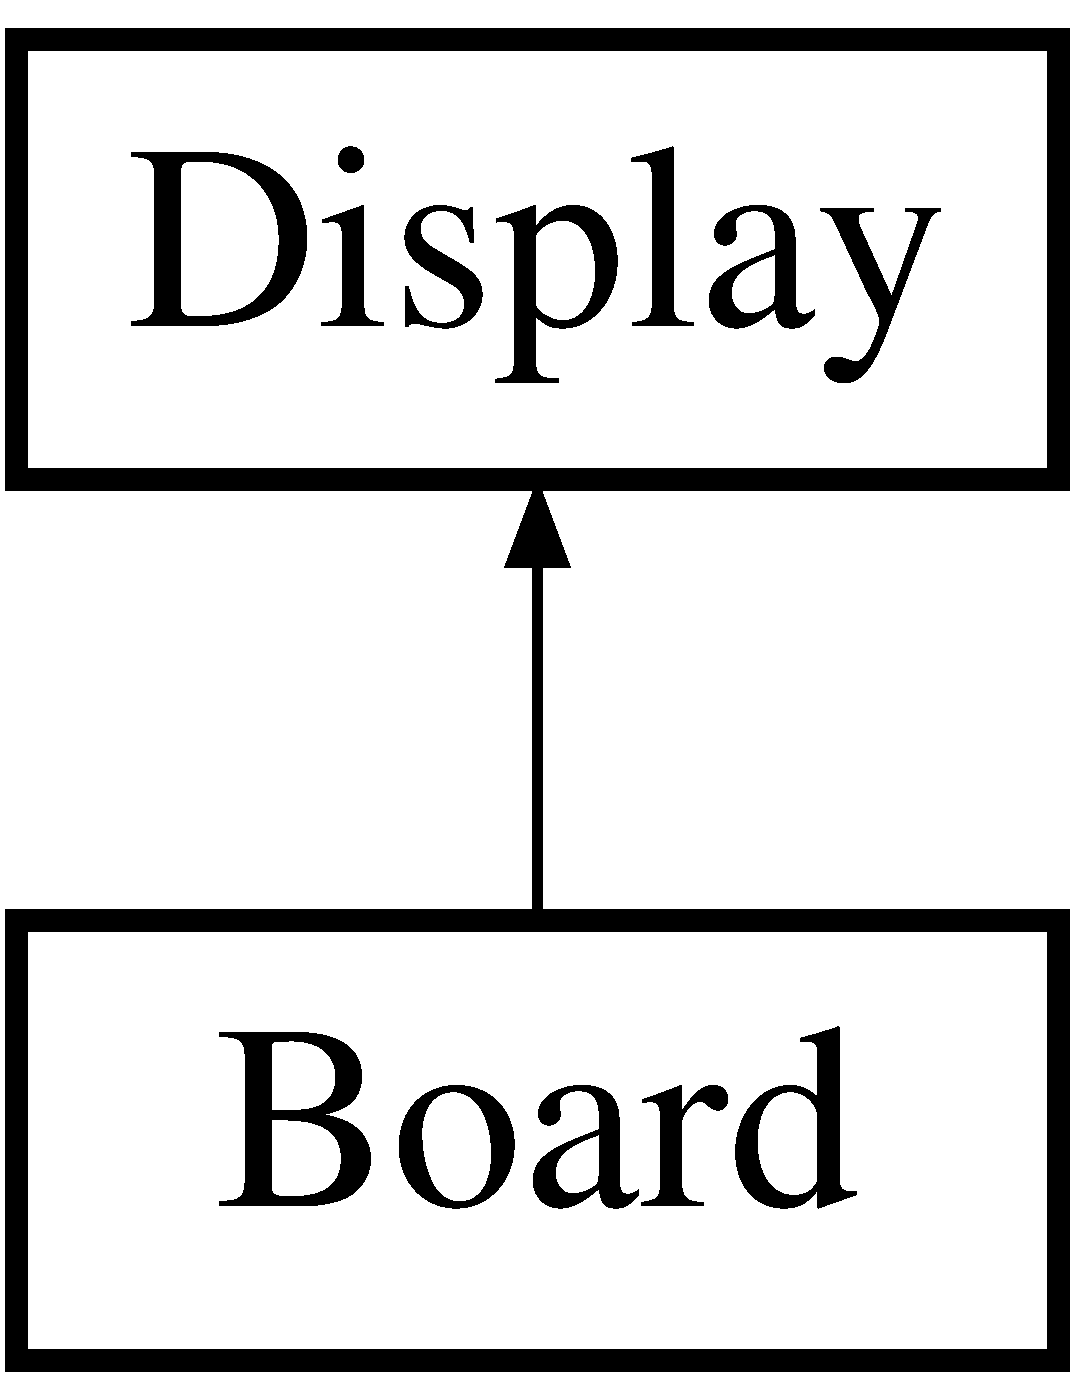
\includegraphics[height=2.000000cm]{classBoard}
\end{center}
\end{figure}
\subsection*{Membres hérités additionnels}


La documentation de cette classe a été générée à partir du fichier suivant \+:\begin{DoxyCompactItemize}
\item 
client/\hyperlink{Board_8hpp}{Board.\+hpp}\end{DoxyCompactItemize}

\hypertarget{classCard}{}\section{Référence de la classe Card}
\label{classCard}\index{Card@{Card}}


{\ttfamily \#include $<$Card.\+hpp$>$}

Graphe d\textquotesingle{}héritage de Card\+:\begin{figure}[H]
\begin{center}
\leavevmode
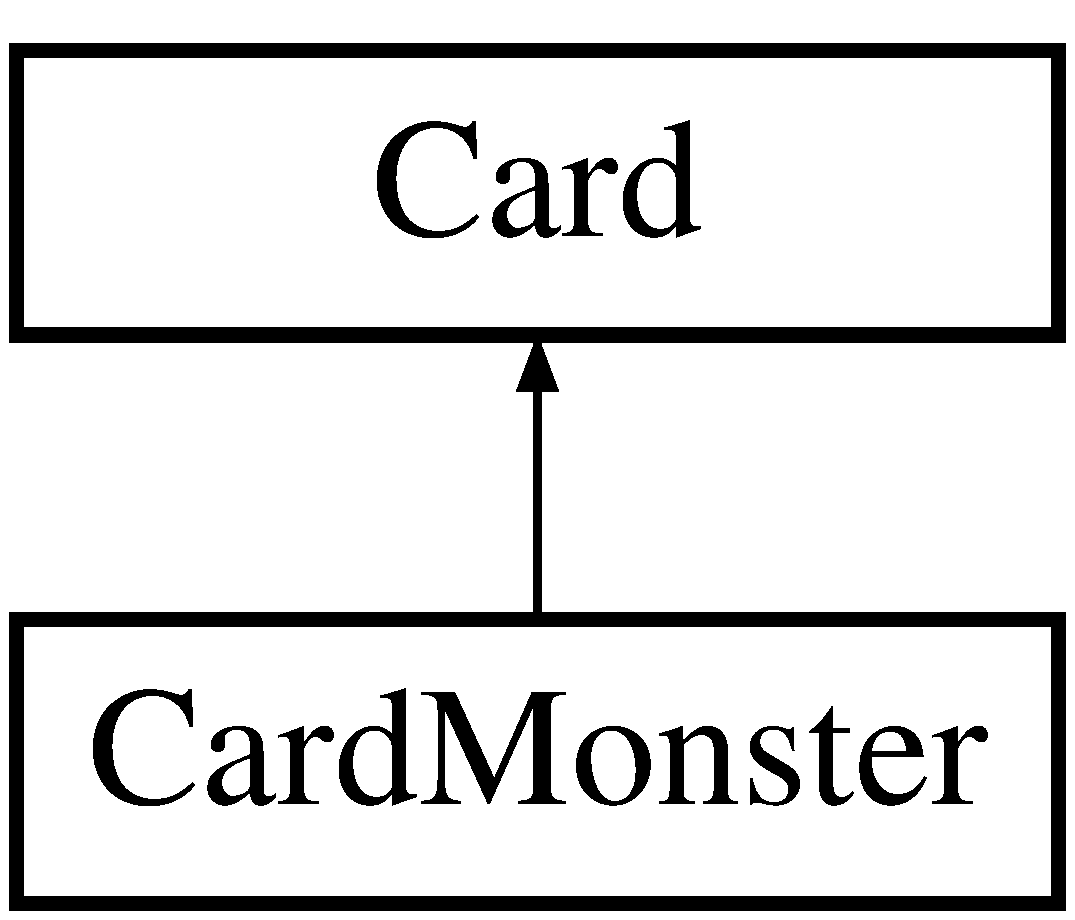
\includegraphics[height=2.000000cm]{classCard}
\end{center}
\end{figure}
\subsection*{Fonctions membres publiques}
\begin{DoxyCompactItemize}
\item 
\hyperlink{classCard_a7697964e07b49437270461cdd1b21f54}{Card} (int id, bool \hyperlink{classCard_a41da498b0822b35dcbb69293851b39fc}{is\+Monster}, std\+::string name, std\+::string description, std\+::size\+\_\+t energy, int H\+P)
\item 
\hyperlink{classCard_a2914c3978ed065d99ec335bc6788e060}{$\sim$\+Card} ()=default
\item 
int \hyperlink{classCard_a017122109ae10b3c0cce6b267f323414}{get\+Id} ()
\item 
bool \hyperlink{classCard_a41da498b0822b35dcbb69293851b39fc}{is\+Monster} ()
\item 
std\+::string \hyperlink{classCard_ad060fe107bfaf4741c671615885b314a}{get\+Name} ()
\item 
std\+::string \hyperlink{classCard_a9ffcf78c4078240a1c454f972420e5ba}{get\+Description} ()
\item 
int \hyperlink{classCard_a8e4e806367f17a15673abf8b9aea9503}{get\+Energy\+Cost} ()
\item 
int \hyperlink{classCard_a6923e2fb5d6c193195f3a5ccef7d73d8}{get\+Max\+H\+P} ()
\item 
int \hyperlink{classCard_abf23a8fc4f0b6b75bc077385735502cc}{get\+H\+P} ()
\item 
\hyperlink{classCard_a93a01fd515bd91db24f7e0a3eb93d7d9}{Card} (unsigned int id, std\+::string name, unsigned int energy, int effect, bool)
\item 
\hyperlink{classCard_ae3384913af007a1c1a536228778da6b0}{Card} (\hyperlink{classCard}{Card} \&card)=default
\item 
\hyperlink{classCard}{Card} \& \hyperlink{classCard_a61af6ac06f1d73616a7e9b4a1b19c90d}{operator=} (const \hyperlink{classCard}{Card} \&)=default
\item 
virtual void \hyperlink{classCard_a68c2becce15d5c89cec9972a8674e602}{apply\+Effect} (\hyperlink{classCardMonster}{Card\+Monster} \&cardmonster, \hyperlink{classGame}{Game} \&)
\item 
virtual void \hyperlink{classCard_a0ee99642963ac428501623982a21aa1b}{apply\+Effect} (\hyperlink{classPlayerInGame}{Player\+In\+Game} \&player, \hyperlink{classGame}{Game} \&)
\item 
virtual \hyperlink{classCard_a2b09fd7321b238b45b2ad2f034760e5d}{$\sim$\+Card} ()
\item 
unsigned int \hyperlink{classCard_aacf1e4fc22c1e1d6f6fc72075a940882}{get\+Id} () const 
\item 
std\+::string \hyperlink{classCard_a72b894bbe15fedc2f43ea9810dc111d9}{get\+Name} () const 
\item 
unsigned int \hyperlink{classCard_aeb9f6c68f55851343dc35428b7920fde}{get\+Energy\+Cost} ()
\item 
bool \hyperlink{classCard_a9932401135454db169e1e4d678103917}{got\+Effect} ()
\item 
int \hyperlink{classCard_a6f6c3220c269eef98fe84ffbcffd9371}{get\+Effect\+I\+D} ()
\item 
virtual bool \hyperlink{classCard_a75c94d383b9710efb023de601b7103c5}{is\+Monster} ()
\item 
virtual bool \hyperlink{classCard_a0f6b9524f9af3386013d9d6324256acf}{can\+Be\+Apply\+On\+Card} ()
\item 
virtual bool \hyperlink{classCard_a81da86fdfe5ab43869f8d64c28fb4462}{can\+Be\+Apply\+On\+Player} ()
\end{DoxyCompactItemize}


\subsection{Description détaillée}
One class per card. Contain all information of the card 

\subsection{Documentation des constructeurs et destructeur}
\hypertarget{classCard_a7697964e07b49437270461cdd1b21f54}{}\index{Card@{Card}!Card@{Card}}
\index{Card@{Card}!Card@{Card}}
\subsubsection[{Card(int id, bool is\+Monster, std\+::string name, std\+::string description, std\+::size\+\_\+t energy, int H\+P)}]{\setlength{\rightskip}{0pt plus 5cm}Card\+::\+Card (
\begin{DoxyParamCaption}
\item[{int}]{id, }
\item[{bool}]{is\+Monster, }
\item[{std\+::string}]{name, }
\item[{std\+::string}]{description, }
\item[{std\+::size\+\_\+t}]{energy, }
\item[{int}]{H\+P}
\end{DoxyParamCaption}
)\hspace{0.3cm}{\ttfamily [inline]}}\label{classCard_a7697964e07b49437270461cdd1b21f54}
\hypertarget{classCard_a2914c3978ed065d99ec335bc6788e060}{}\index{Card@{Card}!````~Card@{$\sim$\+Card}}
\index{````~Card@{$\sim$\+Card}!Card@{Card}}
\subsubsection[{$\sim$\+Card()=default}]{\setlength{\rightskip}{0pt plus 5cm}Card\+::$\sim$\+Card (
\begin{DoxyParamCaption}
{}
\end{DoxyParamCaption}
)\hspace{0.3cm}{\ttfamily [default]}}\label{classCard_a2914c3978ed065d99ec335bc6788e060}
\hypertarget{classCard_a93a01fd515bd91db24f7e0a3eb93d7d9}{}\index{Card@{Card}!Card@{Card}}
\index{Card@{Card}!Card@{Card}}
\subsubsection[{Card(unsigned int id, std\+::string name, unsigned int energy, int effect, bool)}]{\setlength{\rightskip}{0pt plus 5cm}Card\+::\+Card (
\begin{DoxyParamCaption}
\item[{unsigned int}]{id, }
\item[{std\+::string}]{name, }
\item[{unsigned int}]{energy, }
\item[{int}]{effect, }
\item[{bool}]{save = {\ttfamily true}}
\end{DoxyParamCaption}
)}\label{classCard_a93a01fd515bd91db24f7e0a3eb93d7d9}
Constructor


\begin{DoxyParams}{Paramètres}
{\em id} & of the card \\
\hline
{\em name} & of the card \\
\hline
{\em energy} & of the card \\
\hline
{\em effect} & name of the specific effect \\
\hline
{\em save} & True if save in cache \\
\hline
\end{DoxyParams}
\hypertarget{classCard_ae3384913af007a1c1a536228778da6b0}{}\index{Card@{Card}!Card@{Card}}
\index{Card@{Card}!Card@{Card}}
\subsubsection[{Card(\+Card \&card)=default}]{\setlength{\rightskip}{0pt plus 5cm}Card\+::\+Card (
\begin{DoxyParamCaption}
\item[{{\bf Card} \&}]{card}
\end{DoxyParamCaption}
)\hspace{0.3cm}{\ttfamily [default]}}\label{classCard_ae3384913af007a1c1a536228778da6b0}
\hypertarget{classCard_a2b09fd7321b238b45b2ad2f034760e5d}{}\index{Card@{Card}!````~Card@{$\sim$\+Card}}
\index{````~Card@{$\sim$\+Card}!Card@{Card}}
\subsubsection[{$\sim$\+Card()}]{\setlength{\rightskip}{0pt plus 5cm}virtual Card\+::$\sim$\+Card (
\begin{DoxyParamCaption}
{}
\end{DoxyParamCaption}
)\hspace{0.3cm}{\ttfamily [virtual]}}\label{classCard_a2b09fd7321b238b45b2ad2f034760e5d}


\subsection{Documentation des fonctions membres}
\hypertarget{classCard_a68c2becce15d5c89cec9972a8674e602}{}\index{Card@{Card}!apply\+Effect@{apply\+Effect}}
\index{apply\+Effect@{apply\+Effect}!Card@{Card}}
\subsubsection[{apply\+Effect(\+Card\+Monster \&cardmonster, Game \&)}]{\setlength{\rightskip}{0pt plus 5cm}void Card\+::apply\+Effect (
\begin{DoxyParamCaption}
\item[{{\bf Card\+Monster} \&}]{cardmonster, }
\item[{{\bf Game} \&}]{game}
\end{DoxyParamCaption}
)\hspace{0.3cm}{\ttfamily [virtual]}}\label{classCard_a68c2becce15d5c89cec9972a8674e602}
Apply the effect on a monster


\begin{DoxyParams}{Paramètres}
{\em the} & monster targeted \\
\hline
{\em the} & game where the effect will be apply \\
\hline
\end{DoxyParams}
\begin{DoxyReturn}{Renvoie}
void 
\end{DoxyReturn}
\hypertarget{classCard_a0ee99642963ac428501623982a21aa1b}{}\index{Card@{Card}!apply\+Effect@{apply\+Effect}}
\index{apply\+Effect@{apply\+Effect}!Card@{Card}}
\subsubsection[{apply\+Effect(\+Player\+In\+Game \&player, Game \&)}]{\setlength{\rightskip}{0pt plus 5cm}void Card\+::apply\+Effect (
\begin{DoxyParamCaption}
\item[{{\bf Player\+In\+Game} \&}]{player, }
\item[{{\bf Game} \&}]{game}
\end{DoxyParamCaption}
)\hspace{0.3cm}{\ttfamily [virtual]}}\label{classCard_a0ee99642963ac428501623982a21aa1b}
Apply the effect on a player


\begin{DoxyParams}{Paramètres}
{\em the} & player targeted \\
\hline
{\em the} & game where the effect will be apply \\
\hline
\end{DoxyParams}
\begin{DoxyReturn}{Renvoie}
void 
\end{DoxyReturn}
\hypertarget{classCard_a0f6b9524f9af3386013d9d6324256acf}{}\index{Card@{Card}!can\+Be\+Apply\+On\+Card@{can\+Be\+Apply\+On\+Card}}
\index{can\+Be\+Apply\+On\+Card@{can\+Be\+Apply\+On\+Card}!Card@{Card}}
\subsubsection[{can\+Be\+Apply\+On\+Card()}]{\setlength{\rightskip}{0pt plus 5cm}bool Card\+::can\+Be\+Apply\+On\+Card (
\begin{DoxyParamCaption}
{}
\end{DoxyParamCaption}
)\hspace{0.3cm}{\ttfamily [virtual]}}\label{classCard_a0f6b9524f9af3386013d9d6324256acf}
Check if the effect can be apply on a player

\begin{DoxyReturn}{Renvoie}
true if yes, false if not 
\end{DoxyReturn}
\hypertarget{classCard_a81da86fdfe5ab43869f8d64c28fb4462}{}\index{Card@{Card}!can\+Be\+Apply\+On\+Player@{can\+Be\+Apply\+On\+Player}}
\index{can\+Be\+Apply\+On\+Player@{can\+Be\+Apply\+On\+Player}!Card@{Card}}
\subsubsection[{can\+Be\+Apply\+On\+Player()}]{\setlength{\rightskip}{0pt plus 5cm}bool Card\+::can\+Be\+Apply\+On\+Player (
\begin{DoxyParamCaption}
{}
\end{DoxyParamCaption}
)\hspace{0.3cm}{\ttfamily [virtual]}}\label{classCard_a81da86fdfe5ab43869f8d64c28fb4462}
Check if the effect can be apply on a player

\begin{DoxyReturn}{Renvoie}
true if yes, false if not 
\end{DoxyReturn}
\hypertarget{classCard_a9ffcf78c4078240a1c454f972420e5ba}{}\index{Card@{Card}!get\+Description@{get\+Description}}
\index{get\+Description@{get\+Description}!Card@{Card}}
\subsubsection[{get\+Description()}]{\setlength{\rightskip}{0pt plus 5cm}std\+::string Card\+::get\+Description (
\begin{DoxyParamCaption}
{}
\end{DoxyParamCaption}
)\hspace{0.3cm}{\ttfamily [inline]}}\label{classCard_a9ffcf78c4078240a1c454f972420e5ba}
\hypertarget{classCard_a6f6c3220c269eef98fe84ffbcffd9371}{}\index{Card@{Card}!get\+Effect\+I\+D@{get\+Effect\+I\+D}}
\index{get\+Effect\+I\+D@{get\+Effect\+I\+D}!Card@{Card}}
\subsubsection[{get\+Effect\+I\+D()}]{\setlength{\rightskip}{0pt plus 5cm}int Card\+::get\+Effect\+I\+D (
\begin{DoxyParamCaption}
{}
\end{DoxyParamCaption}
)}\label{classCard_a6f6c3220c269eef98fe84ffbcffd9371}
Return the effect id

\begin{DoxyReturn}{Renvoie}
-\/1 if no effect or the effect id 
\end{DoxyReturn}
\hypertarget{classCard_a8e4e806367f17a15673abf8b9aea9503}{}\index{Card@{Card}!get\+Energy\+Cost@{get\+Energy\+Cost}}
\index{get\+Energy\+Cost@{get\+Energy\+Cost}!Card@{Card}}
\subsubsection[{get\+Energy\+Cost()}]{\setlength{\rightskip}{0pt plus 5cm}int Card\+::get\+Energy\+Cost (
\begin{DoxyParamCaption}
{}
\end{DoxyParamCaption}
)\hspace{0.3cm}{\ttfamily [inline]}}\label{classCard_a8e4e806367f17a15673abf8b9aea9503}
\hypertarget{classCard_aeb9f6c68f55851343dc35428b7920fde}{}\index{Card@{Card}!get\+Energy\+Cost@{get\+Energy\+Cost}}
\index{get\+Energy\+Cost@{get\+Energy\+Cost}!Card@{Card}}
\subsubsection[{get\+Energy\+Cost()}]{\setlength{\rightskip}{0pt plus 5cm}unsigned int Card\+::get\+Energy\+Cost (
\begin{DoxyParamCaption}
{}
\end{DoxyParamCaption}
)\hspace{0.3cm}{\ttfamily [inline]}}\label{classCard_aeb9f6c68f55851343dc35428b7920fde}
\hypertarget{classCard_abf23a8fc4f0b6b75bc077385735502cc}{}\index{Card@{Card}!get\+H\+P@{get\+H\+P}}
\index{get\+H\+P@{get\+H\+P}!Card@{Card}}
\subsubsection[{get\+H\+P()}]{\setlength{\rightskip}{0pt plus 5cm}int Card\+::get\+H\+P (
\begin{DoxyParamCaption}
{}
\end{DoxyParamCaption}
)\hspace{0.3cm}{\ttfamily [inline]}}\label{classCard_abf23a8fc4f0b6b75bc077385735502cc}
\hypertarget{classCard_a017122109ae10b3c0cce6b267f323414}{}\index{Card@{Card}!get\+Id@{get\+Id}}
\index{get\+Id@{get\+Id}!Card@{Card}}
\subsubsection[{get\+Id()}]{\setlength{\rightskip}{0pt plus 5cm}int Card\+::get\+Id (
\begin{DoxyParamCaption}
{}
\end{DoxyParamCaption}
)\hspace{0.3cm}{\ttfamily [inline]}}\label{classCard_a017122109ae10b3c0cce6b267f323414}
\hypertarget{classCard_aacf1e4fc22c1e1d6f6fc72075a940882}{}\index{Card@{Card}!get\+Id@{get\+Id}}
\index{get\+Id@{get\+Id}!Card@{Card}}
\subsubsection[{get\+Id() const }]{\setlength{\rightskip}{0pt plus 5cm}unsigned int Card\+::get\+Id (
\begin{DoxyParamCaption}
{}
\end{DoxyParamCaption}
) const\hspace{0.3cm}{\ttfamily [inline]}}\label{classCard_aacf1e4fc22c1e1d6f6fc72075a940882}
\hypertarget{classCard_a6923e2fb5d6c193195f3a5ccef7d73d8}{}\index{Card@{Card}!get\+Max\+H\+P@{get\+Max\+H\+P}}
\index{get\+Max\+H\+P@{get\+Max\+H\+P}!Card@{Card}}
\subsubsection[{get\+Max\+H\+P()}]{\setlength{\rightskip}{0pt plus 5cm}int Card\+::get\+Max\+H\+P (
\begin{DoxyParamCaption}
{}
\end{DoxyParamCaption}
)\hspace{0.3cm}{\ttfamily [inline]}}\label{classCard_a6923e2fb5d6c193195f3a5ccef7d73d8}
\hypertarget{classCard_ad060fe107bfaf4741c671615885b314a}{}\index{Card@{Card}!get\+Name@{get\+Name}}
\index{get\+Name@{get\+Name}!Card@{Card}}
\subsubsection[{get\+Name()}]{\setlength{\rightskip}{0pt plus 5cm}std\+::string Card\+::get\+Name (
\begin{DoxyParamCaption}
{}
\end{DoxyParamCaption}
)\hspace{0.3cm}{\ttfamily [inline]}}\label{classCard_ad060fe107bfaf4741c671615885b314a}
\hypertarget{classCard_a72b894bbe15fedc2f43ea9810dc111d9}{}\index{Card@{Card}!get\+Name@{get\+Name}}
\index{get\+Name@{get\+Name}!Card@{Card}}
\subsubsection[{get\+Name() const }]{\setlength{\rightskip}{0pt plus 5cm}std\+::string Card\+::get\+Name (
\begin{DoxyParamCaption}
{}
\end{DoxyParamCaption}
) const\hspace{0.3cm}{\ttfamily [inline]}}\label{classCard_a72b894bbe15fedc2f43ea9810dc111d9}
\hypertarget{classCard_a9932401135454db169e1e4d678103917}{}\index{Card@{Card}!got\+Effect@{got\+Effect}}
\index{got\+Effect@{got\+Effect}!Card@{Card}}
\subsubsection[{got\+Effect()}]{\setlength{\rightskip}{0pt plus 5cm}bool Card\+::got\+Effect (
\begin{DoxyParamCaption}
{}
\end{DoxyParamCaption}
)}\label{classCard_a9932401135454db169e1e4d678103917}
Check if the card got an effect

\begin{DoxyReturn}{Renvoie}
true if yes, false if not 
\end{DoxyReturn}
\hypertarget{classCard_a41da498b0822b35dcbb69293851b39fc}{}\index{Card@{Card}!is\+Monster@{is\+Monster}}
\index{is\+Monster@{is\+Monster}!Card@{Card}}
\subsubsection[{is\+Monster()}]{\setlength{\rightskip}{0pt plus 5cm}bool Card\+::is\+Monster (
\begin{DoxyParamCaption}
{}
\end{DoxyParamCaption}
)\hspace{0.3cm}{\ttfamily [inline]}}\label{classCard_a41da498b0822b35dcbb69293851b39fc}
\hypertarget{classCard_a75c94d383b9710efb023de601b7103c5}{}\index{Card@{Card}!is\+Monster@{is\+Monster}}
\index{is\+Monster@{is\+Monster}!Card@{Card}}
\subsubsection[{is\+Monster()}]{\setlength{\rightskip}{0pt plus 5cm}virtual bool Card\+::is\+Monster (
\begin{DoxyParamCaption}
{}
\end{DoxyParamCaption}
)\hspace{0.3cm}{\ttfamily [inline]}, {\ttfamily [virtual]}}\label{classCard_a75c94d383b9710efb023de601b7103c5}


Réimplémentée dans \hyperlink{classCardMonster_add70449c1bc34baee852fe07cc7d39cc}{Card\+Monster}.

\hypertarget{classCard_a61af6ac06f1d73616a7e9b4a1b19c90d}{}\index{Card@{Card}!operator=@{operator=}}
\index{operator=@{operator=}!Card@{Card}}
\subsubsection[{operator=(const Card \&)=default}]{\setlength{\rightskip}{0pt plus 5cm}{\bf Card}\& Card\+::operator= (
\begin{DoxyParamCaption}
\item[{const {\bf Card} \&}]{}
\end{DoxyParamCaption}
)\hspace{0.3cm}{\ttfamily [default]}}\label{classCard_a61af6ac06f1d73616a7e9b4a1b19c90d}


La documentation de cette classe a été générée à partir des fichiers suivants \+:\begin{DoxyCompactItemize}
\item 
client/\hyperlink{client_2Card_8hpp}{Card.\+hpp}\item 
server/\hyperlink{Card_8cpp}{Card.\+cpp}\end{DoxyCompactItemize}

\hypertarget{classCardManager}{}\section{Référence de la classe Card\+Manager}
\label{classCardManager}\index{Card\+Manager@{Card\+Manager}}


{\ttfamily \#include $<$Card\+Manager.\+hpp$>$}

\subsection*{Fonctions membres publiques statiques}
\begin{DoxyCompactItemize}
\item 
static \hyperlink{classCard}{Card} $\ast$ \hyperlink{classCardManager_a075716c971c02d023a54522f846d9e0a}{get\+Card\+By\+Id} (std\+::size\+\_\+t id)
\item 
static void \hyperlink{classCardManager_ad51c06332d328195fe84aff9aa526272}{load\+All\+Cards} ()
\end{DoxyCompactItemize}


\subsection{Documentation des fonctions membres}
\hypertarget{classCardManager_a075716c971c02d023a54522f846d9e0a}{}\index{Card\+Manager@{Card\+Manager}!get\+Card\+By\+Id@{get\+Card\+By\+Id}}
\index{get\+Card\+By\+Id@{get\+Card\+By\+Id}!Card\+Manager@{Card\+Manager}}
\subsubsection[{get\+Card\+By\+Id(std\+::size\+\_\+t id)}]{\setlength{\rightskip}{0pt plus 5cm}static {\bf Card}$\ast$ Card\+Manager\+::get\+Card\+By\+Id (
\begin{DoxyParamCaption}
\item[{std\+::size\+\_\+t}]{id}
\end{DoxyParamCaption}
)\hspace{0.3cm}{\ttfamily [static]}}\label{classCardManager_a075716c971c02d023a54522f846d9e0a}
\hypertarget{classCardManager_ad51c06332d328195fe84aff9aa526272}{}\index{Card\+Manager@{Card\+Manager}!load\+All\+Cards@{load\+All\+Cards}}
\index{load\+All\+Cards@{load\+All\+Cards}!Card\+Manager@{Card\+Manager}}
\subsubsection[{load\+All\+Cards()}]{\setlength{\rightskip}{0pt plus 5cm}void Card\+Manager\+::load\+All\+Cards (
\begin{DoxyParamCaption}
{}
\end{DoxyParamCaption}
)\hspace{0.3cm}{\ttfamily [static]}}\label{classCardManager_ad51c06332d328195fe84aff9aa526272}
Get the card object in cache


\begin{DoxyParams}{Paramètres}
{\em id} & of the card \\
\hline
\end{DoxyParams}
\begin{DoxyReturn}{Renvoie}
the card or nullptr if doesn\textquotesingle{}t exist 
\end{DoxyReturn}


La documentation de cette classe a été générée à partir des fichiers suivants \+:\begin{DoxyCompactItemize}
\item 
server/\hyperlink{CardManager_8hpp}{Card\+Manager.\+hpp}\item 
server/\hyperlink{CardManager_8cpp}{Card\+Manager.\+cpp}\end{DoxyCompactItemize}

\hypertarget{classCardMonster}{}\section{Référence de la classe Card\+Monster}
\label{classCardMonster}\index{Card\+Monster@{Card\+Monster}}


{\ttfamily \#include $<$Card\+Monster.\+hpp$>$}

Graphe d\textquotesingle{}héritage de Card\+Monster\+:\begin{figure}[H]
\begin{center}
\leavevmode
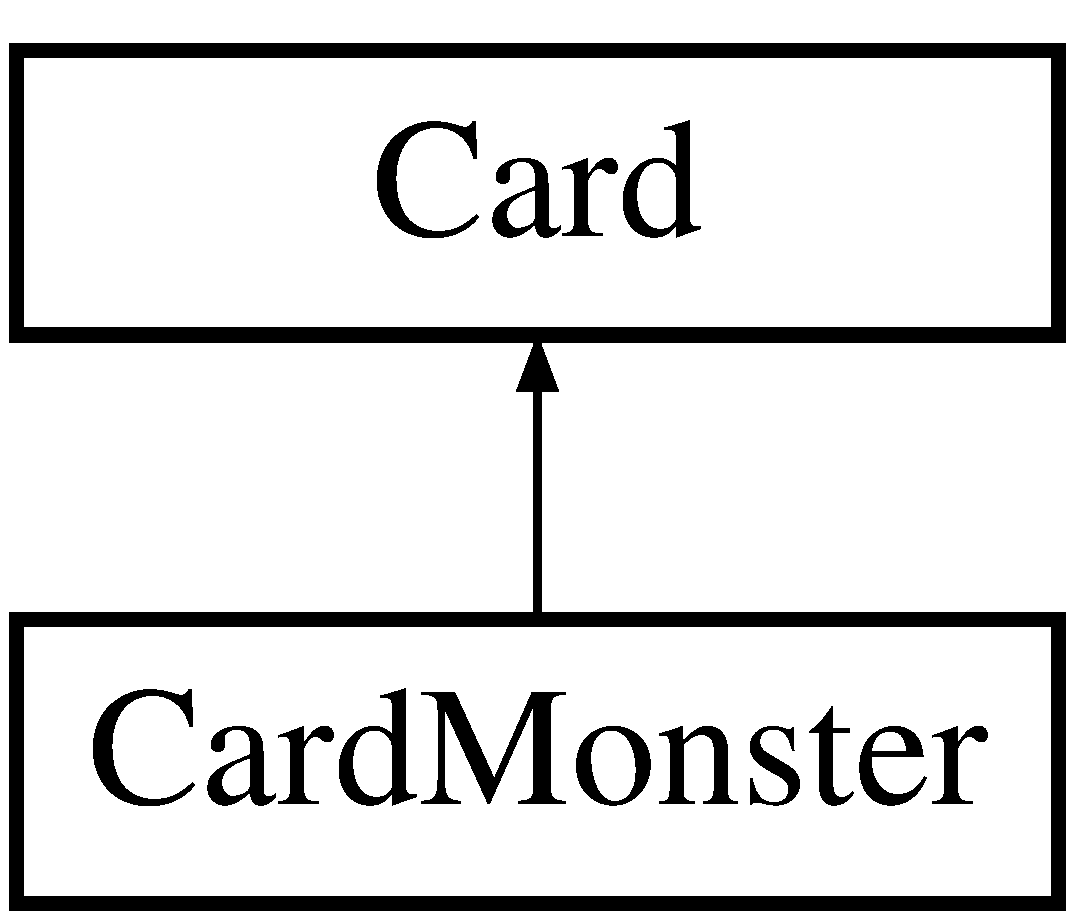
\includegraphics[height=2.000000cm]{classCardMonster}
\end{center}
\end{figure}
\subsection*{Fonctions membres publiques}
\begin{DoxyCompactItemize}
\item 
virtual void \hyperlink{classCardMonster_aaf28396b394a9400d257eddfa09e4567}{deal\+Damage} (\hyperlink{classCardMonster}{Card\+Monster} \&other\+Monster)
\item 
virtual void \hyperlink{classCardMonster_a829d68246c3af5f136cdf2cbc11284b0}{deal\+Damage} (\hyperlink{classPlayerInGame}{Player\+In\+Game} \&player)
\item 
virtual void \hyperlink{classCardMonster_a2d55cf30d111437486e2b1bacefcbf79}{increment\+Tour} ()
\item 
\hyperlink{classCardMonster_a0a48a188d85c6e95a109638be09ddbca}{Card\+Monster} (std\+::size\+\_\+t id, std\+::string name, std\+::size\+\_\+t energy, int effect, bool, std\+::size\+\_\+t life, std\+::size\+\_\+t attack, std\+::size\+\_\+t nbr\+Tour=0)
\item 
\hyperlink{classCardMonster_a5f577cbecdf0d1c6a6ccbc848793ddef}{Card\+Monster} (\hyperlink{classCardMonster}{Card\+Monster} \&other\+Monster)
\item 
std\+::size\+\_\+t \hyperlink{classCardMonster_a01f20967b3b350e8430c30396c8cd0c9}{get\+Life} ()
\item 
std\+::size\+\_\+t \hyperlink{classCardMonster_a38fd3549de7e606f73e836ba98ed4f24}{get\+Attack} ()
\item 
std\+::size\+\_\+t \hyperlink{classCardMonster_a0e963cc2c613826e28891f00a9787e58}{get\+Max\+Life} ()
\item 
std\+::size\+\_\+t \hyperlink{classCardMonster_a8f3fd5d1e30a520aaa0c282bd84aa5d5}{get\+Nbr\+Tour\+Pose} ()
\item 
virtual bool \hyperlink{classCardMonster_add70449c1bc34baee852fe07cc7d39cc}{is\+Monster} () override
\item 
void \hyperlink{classCardMonster_aa70aa05b038da703524b82df5608734b}{set\+Life} (std\+::size\+\_\+t new\+Life)
\item 
void \hyperlink{classCardMonster_a358474586372d6b2b83301cceae34347}{set\+Attack} (std\+::size\+\_\+t new\+Attack)
\item 
void \hyperlink{classCardMonster_a9860956677866c7adbcda61c9951dd35}{set\+Max\+Life} (std\+::size\+\_\+t new\+Max)
\item 
bool \hyperlink{classCardMonster_a53aedfc1c1b823c775f3437685428d70}{is\+Death} ()
\end{DoxyCompactItemize}


\subsection{Documentation des constructeurs et destructeur}
\hypertarget{classCardMonster_a0a48a188d85c6e95a109638be09ddbca}{}\index{Card\+Monster@{Card\+Monster}!Card\+Monster@{Card\+Monster}}
\index{Card\+Monster@{Card\+Monster}!Card\+Monster@{Card\+Monster}}
\subsubsection[{Card\+Monster(std\+::size\+\_\+t id, std\+::string name, std\+::size\+\_\+t energy, int effect, bool, std\+::size\+\_\+t life, std\+::size\+\_\+t attack, std\+::size\+\_\+t nbr\+Tour=0)}]{\setlength{\rightskip}{0pt plus 5cm}Card\+Monster\+::\+Card\+Monster (
\begin{DoxyParamCaption}
\item[{std\+::size\+\_\+t}]{id, }
\item[{std\+::string}]{name, }
\item[{std\+::size\+\_\+t}]{energy, }
\item[{int}]{effect, }
\item[{bool}]{a\+Bool, }
\item[{std\+::size\+\_\+t}]{life, }
\item[{std\+::size\+\_\+t}]{attack, }
\item[{std\+::size\+\_\+t}]{nbr\+Tour = {\ttfamily 0}}
\end{DoxyParamCaption}
)}\label{classCardMonster_a0a48a188d85c6e95a109638be09ddbca}
\hypertarget{classCardMonster_a5f577cbecdf0d1c6a6ccbc848793ddef}{}\index{Card\+Monster@{Card\+Monster}!Card\+Monster@{Card\+Monster}}
\index{Card\+Monster@{Card\+Monster}!Card\+Monster@{Card\+Monster}}
\subsubsection[{Card\+Monster(\+Card\+Monster \&other\+Monster)}]{\setlength{\rightskip}{0pt plus 5cm}Card\+Monster\+::\+Card\+Monster (
\begin{DoxyParamCaption}
\item[{{\bf Card\+Monster} \&}]{other\+Monster}
\end{DoxyParamCaption}
)}\label{classCardMonster_a5f577cbecdf0d1c6a6ccbc848793ddef}


\subsection{Documentation des fonctions membres}
\hypertarget{classCardMonster_aaf28396b394a9400d257eddfa09e4567}{}\index{Card\+Monster@{Card\+Monster}!deal\+Damage@{deal\+Damage}}
\index{deal\+Damage@{deal\+Damage}!Card\+Monster@{Card\+Monster}}
\subsubsection[{deal\+Damage(\+Card\+Monster \&other\+Monster)}]{\setlength{\rightskip}{0pt plus 5cm}void Card\+Monster\+::deal\+Damage (
\begin{DoxyParamCaption}
\item[{{\bf Card\+Monster} \&}]{other\+Monster}
\end{DoxyParamCaption}
)\hspace{0.3cm}{\ttfamily [virtual]}}\label{classCardMonster_aaf28396b394a9400d257eddfa09e4567}
\hypertarget{classCardMonster_a829d68246c3af5f136cdf2cbc11284b0}{}\index{Card\+Monster@{Card\+Monster}!deal\+Damage@{deal\+Damage}}
\index{deal\+Damage@{deal\+Damage}!Card\+Monster@{Card\+Monster}}
\subsubsection[{deal\+Damage(\+Player\+In\+Game \&player)}]{\setlength{\rightskip}{0pt plus 5cm}void Card\+Monster\+::deal\+Damage (
\begin{DoxyParamCaption}
\item[{{\bf Player\+In\+Game} \&}]{player}
\end{DoxyParamCaption}
)\hspace{0.3cm}{\ttfamily [virtual]}}\label{classCardMonster_a829d68246c3af5f136cdf2cbc11284b0}
\hypertarget{classCardMonster_a38fd3549de7e606f73e836ba98ed4f24}{}\index{Card\+Monster@{Card\+Monster}!get\+Attack@{get\+Attack}}
\index{get\+Attack@{get\+Attack}!Card\+Monster@{Card\+Monster}}
\subsubsection[{get\+Attack()}]{\setlength{\rightskip}{0pt plus 5cm}std\+::size\+\_\+t Card\+Monster\+::get\+Attack (
\begin{DoxyParamCaption}
{}
\end{DoxyParamCaption}
)\hspace{0.3cm}{\ttfamily [inline]}}\label{classCardMonster_a38fd3549de7e606f73e836ba98ed4f24}
\hypertarget{classCardMonster_a01f20967b3b350e8430c30396c8cd0c9}{}\index{Card\+Monster@{Card\+Monster}!get\+Life@{get\+Life}}
\index{get\+Life@{get\+Life}!Card\+Monster@{Card\+Monster}}
\subsubsection[{get\+Life()}]{\setlength{\rightskip}{0pt plus 5cm}std\+::size\+\_\+t Card\+Monster\+::get\+Life (
\begin{DoxyParamCaption}
{}
\end{DoxyParamCaption}
)\hspace{0.3cm}{\ttfamily [inline]}}\label{classCardMonster_a01f20967b3b350e8430c30396c8cd0c9}
\hypertarget{classCardMonster_a0e963cc2c613826e28891f00a9787e58}{}\index{Card\+Monster@{Card\+Monster}!get\+Max\+Life@{get\+Max\+Life}}
\index{get\+Max\+Life@{get\+Max\+Life}!Card\+Monster@{Card\+Monster}}
\subsubsection[{get\+Max\+Life()}]{\setlength{\rightskip}{0pt plus 5cm}std\+::size\+\_\+t Card\+Monster\+::get\+Max\+Life (
\begin{DoxyParamCaption}
{}
\end{DoxyParamCaption}
)\hspace{0.3cm}{\ttfamily [inline]}}\label{classCardMonster_a0e963cc2c613826e28891f00a9787e58}
\hypertarget{classCardMonster_a8f3fd5d1e30a520aaa0c282bd84aa5d5}{}\index{Card\+Monster@{Card\+Monster}!get\+Nbr\+Tour\+Pose@{get\+Nbr\+Tour\+Pose}}
\index{get\+Nbr\+Tour\+Pose@{get\+Nbr\+Tour\+Pose}!Card\+Monster@{Card\+Monster}}
\subsubsection[{get\+Nbr\+Tour\+Pose()}]{\setlength{\rightskip}{0pt plus 5cm}std\+::size\+\_\+t Card\+Monster\+::get\+Nbr\+Tour\+Pose (
\begin{DoxyParamCaption}
{}
\end{DoxyParamCaption}
)\hspace{0.3cm}{\ttfamily [inline]}}\label{classCardMonster_a8f3fd5d1e30a520aaa0c282bd84aa5d5}
\hypertarget{classCardMonster_a2d55cf30d111437486e2b1bacefcbf79}{}\index{Card\+Monster@{Card\+Monster}!increment\+Tour@{increment\+Tour}}
\index{increment\+Tour@{increment\+Tour}!Card\+Monster@{Card\+Monster}}
\subsubsection[{increment\+Tour()}]{\setlength{\rightskip}{0pt plus 5cm}void Card\+Monster\+::increment\+Tour (
\begin{DoxyParamCaption}
{}
\end{DoxyParamCaption}
)\hspace{0.3cm}{\ttfamily [virtual]}}\label{classCardMonster_a2d55cf30d111437486e2b1bacefcbf79}
\hypertarget{classCardMonster_a53aedfc1c1b823c775f3437685428d70}{}\index{Card\+Monster@{Card\+Monster}!is\+Death@{is\+Death}}
\index{is\+Death@{is\+Death}!Card\+Monster@{Card\+Monster}}
\subsubsection[{is\+Death()}]{\setlength{\rightskip}{0pt plus 5cm}bool Card\+Monster\+::is\+Death (
\begin{DoxyParamCaption}
{}
\end{DoxyParamCaption}
)}\label{classCardMonster_a53aedfc1c1b823c775f3437685428d70}
\hypertarget{classCardMonster_add70449c1bc34baee852fe07cc7d39cc}{}\index{Card\+Monster@{Card\+Monster}!is\+Monster@{is\+Monster}}
\index{is\+Monster@{is\+Monster}!Card\+Monster@{Card\+Monster}}
\subsubsection[{is\+Monster() override}]{\setlength{\rightskip}{0pt plus 5cm}virtual bool Card\+Monster\+::is\+Monster (
\begin{DoxyParamCaption}
{}
\end{DoxyParamCaption}
)\hspace{0.3cm}{\ttfamily [inline]}, {\ttfamily [override]}, {\ttfamily [virtual]}}\label{classCardMonster_add70449c1bc34baee852fe07cc7d39cc}


Réimplémentée à partir de \hyperlink{classCard_a75c94d383b9710efb023de601b7103c5}{Card}.

\hypertarget{classCardMonster_a358474586372d6b2b83301cceae34347}{}\index{Card\+Monster@{Card\+Monster}!set\+Attack@{set\+Attack}}
\index{set\+Attack@{set\+Attack}!Card\+Monster@{Card\+Monster}}
\subsubsection[{set\+Attack(std\+::size\+\_\+t new\+Attack)}]{\setlength{\rightskip}{0pt plus 5cm}void Card\+Monster\+::set\+Attack (
\begin{DoxyParamCaption}
\item[{std\+::size\+\_\+t}]{new\+Attack}
\end{DoxyParamCaption}
)\hspace{0.3cm}{\ttfamily [inline]}}\label{classCardMonster_a358474586372d6b2b83301cceae34347}
\hypertarget{classCardMonster_aa70aa05b038da703524b82df5608734b}{}\index{Card\+Monster@{Card\+Monster}!set\+Life@{set\+Life}}
\index{set\+Life@{set\+Life}!Card\+Monster@{Card\+Monster}}
\subsubsection[{set\+Life(std\+::size\+\_\+t new\+Life)}]{\setlength{\rightskip}{0pt plus 5cm}void Card\+Monster\+::set\+Life (
\begin{DoxyParamCaption}
\item[{std\+::size\+\_\+t}]{new\+Life}
\end{DoxyParamCaption}
)\hspace{0.3cm}{\ttfamily [inline]}}\label{classCardMonster_aa70aa05b038da703524b82df5608734b}
\hypertarget{classCardMonster_a9860956677866c7adbcda61c9951dd35}{}\index{Card\+Monster@{Card\+Monster}!set\+Max\+Life@{set\+Max\+Life}}
\index{set\+Max\+Life@{set\+Max\+Life}!Card\+Monster@{Card\+Monster}}
\subsubsection[{set\+Max\+Life(std\+::size\+\_\+t new\+Max)}]{\setlength{\rightskip}{0pt plus 5cm}void Card\+Monster\+::set\+Max\+Life (
\begin{DoxyParamCaption}
\item[{std\+::size\+\_\+t}]{new\+Max}
\end{DoxyParamCaption}
)\hspace{0.3cm}{\ttfamily [inline]}}\label{classCardMonster_a9860956677866c7adbcda61c9951dd35}


La documentation de cette classe a été générée à partir des fichiers suivants \+:\begin{DoxyCompactItemize}
\item 
common/\hyperlink{CardMonster_8hpp}{Card\+Monster.\+hpp}\item 
common/\hyperlink{CardMonster_8cpp}{Card\+Monster.\+cpp}\end{DoxyCompactItemize}

\hypertarget{structPacket_1_1carteInfosPacket}{}\section{Référence de la structure Packet\+:\+:carte\+Infos\+Packet}
\label{structPacket_1_1carteInfosPacket}\index{Packet\+::carte\+Infos\+Packet@{Packet\+::carte\+Infos\+Packet}}


{\ttfamily \#include $<$Packet.\+hpp$>$}

\subsection*{Attributs publics}
\begin{DoxyCompactItemize}
\item 
int \hyperlink{structPacket_1_1carteInfosPacket_aa385cf584f070650fa90455a9e4d9f90}{I\+D} = \hyperlink{classPacket_ae91c1d355e4c8f0bef5f893747473661aa61d9c1d39512a3a4054cbfc15a60b48}{C\+A\+R\+T\+E\+\_\+\+I\+N\+F\+O\+\_\+\+I\+D}
\item 
int \hyperlink{structPacket_1_1carteInfosPacket_a5b1c8a614c8dcfa1d01d59210bab4d85}{size} = sizeof(int)+sizeof(char)$\ast$\hyperlink{Packet_8hpp_a1de6746763761071cb33e1fbbe574f62}{M\+A\+X\+\_\+\+C\+A\+R\+T\+E\+\_\+\+D\+E\+S\+C\+R\+I\+T\+I\+O\+N\+\_\+\+S\+I\+Z\+E}
\item 
int \hyperlink{structPacket_1_1carteInfosPacket_ac936145974d445b5476f4dec4583498f}{carte\+I\+D}
\item 
char \hyperlink{structPacket_1_1carteInfosPacket_a3b02e4ea49980ee77d5882fcf5f258ba}{cartes\+Description} \mbox{[}\hyperlink{Packet_8hpp_a1de6746763761071cb33e1fbbe574f62}{M\+A\+X\+\_\+\+C\+A\+R\+T\+E\+\_\+\+D\+E\+S\+C\+R\+I\+T\+I\+O\+N\+\_\+\+S\+I\+Z\+E}\mbox{]}
\end{DoxyCompactItemize}


\subsection{Documentation des données membres}
\hypertarget{structPacket_1_1carteInfosPacket_ac936145974d445b5476f4dec4583498f}{}\index{Packet\+::carte\+Infos\+Packet@{Packet\+::carte\+Infos\+Packet}!carte\+I\+D@{carte\+I\+D}}
\index{carte\+I\+D@{carte\+I\+D}!Packet\+::carte\+Infos\+Packet@{Packet\+::carte\+Infos\+Packet}}
\subsubsection[{carte\+I\+D}]{\setlength{\rightskip}{0pt plus 5cm}int Packet\+::carte\+Infos\+Packet\+::carte\+I\+D}\label{structPacket_1_1carteInfosPacket_ac936145974d445b5476f4dec4583498f}
\hypertarget{structPacket_1_1carteInfosPacket_a3b02e4ea49980ee77d5882fcf5f258ba}{}\index{Packet\+::carte\+Infos\+Packet@{Packet\+::carte\+Infos\+Packet}!cartes\+Description@{cartes\+Description}}
\index{cartes\+Description@{cartes\+Description}!Packet\+::carte\+Infos\+Packet@{Packet\+::carte\+Infos\+Packet}}
\subsubsection[{cartes\+Description}]{\setlength{\rightskip}{0pt plus 5cm}char Packet\+::carte\+Infos\+Packet\+::cartes\+Description\mbox{[}{\bf M\+A\+X\+\_\+\+C\+A\+R\+T\+E\+\_\+\+D\+E\+S\+C\+R\+I\+T\+I\+O\+N\+\_\+\+S\+I\+Z\+E}\mbox{]}}\label{structPacket_1_1carteInfosPacket_a3b02e4ea49980ee77d5882fcf5f258ba}
\hypertarget{structPacket_1_1carteInfosPacket_aa385cf584f070650fa90455a9e4d9f90}{}\index{Packet\+::carte\+Infos\+Packet@{Packet\+::carte\+Infos\+Packet}!I\+D@{I\+D}}
\index{I\+D@{I\+D}!Packet\+::carte\+Infos\+Packet@{Packet\+::carte\+Infos\+Packet}}
\subsubsection[{I\+D}]{\setlength{\rightskip}{0pt plus 5cm}int Packet\+::carte\+Infos\+Packet\+::\+I\+D = {\bf C\+A\+R\+T\+E\+\_\+\+I\+N\+F\+O\+\_\+\+I\+D}}\label{structPacket_1_1carteInfosPacket_aa385cf584f070650fa90455a9e4d9f90}
\hypertarget{structPacket_1_1carteInfosPacket_a5b1c8a614c8dcfa1d01d59210bab4d85}{}\index{Packet\+::carte\+Infos\+Packet@{Packet\+::carte\+Infos\+Packet}!size@{size}}
\index{size@{size}!Packet\+::carte\+Infos\+Packet@{Packet\+::carte\+Infos\+Packet}}
\subsubsection[{size}]{\setlength{\rightskip}{0pt plus 5cm}int Packet\+::carte\+Infos\+Packet\+::size = sizeof(int)+sizeof(char)$\ast${\bf M\+A\+X\+\_\+\+C\+A\+R\+T\+E\+\_\+\+D\+E\+S\+C\+R\+I\+T\+I\+O\+N\+\_\+\+S\+I\+Z\+E}}\label{structPacket_1_1carteInfosPacket_a5b1c8a614c8dcfa1d01d59210bab4d85}


La documentation de cette structure a été générée à partir du fichier suivant \+:\begin{DoxyCompactItemize}
\item 
common/\hyperlink{Packet_8hpp}{Packet.\+hpp}\end{DoxyCompactItemize}

\hypertarget{structPacket_1_1carteRequestPacket}{}\section{Référence de la structure Packet\+:\+:carte\+Request\+Packet}
\label{structPacket_1_1carteRequestPacket}\index{Packet\+::carte\+Request\+Packet@{Packet\+::carte\+Request\+Packet}}


{\ttfamily \#include $<$Packet.\+hpp$>$}

\subsection*{Attributs publics}
\begin{DoxyCompactItemize}
\item 
int \hyperlink{structPacket_1_1carteRequestPacket_a02b110bcccb9143360e0fab7650dc142}{I\+D} = \hyperlink{classPacket_ae91c1d355e4c8f0bef5f893747473661a1afad4125bf1222a1b4f3201cb29ab3b}{C\+A\+R\+T\+E\+\_\+\+R\+E\+Q\+\_\+\+I\+D}
\item 
int \hyperlink{structPacket_1_1carteRequestPacket_a9ceed268bd66ee87f7f7ce9735f7cac5}{size} = sizeof(int)
\item 
int \hyperlink{structPacket_1_1carteRequestPacket_a22754892275a0a29e5ccde5fe26ecd14}{carte\+I\+D}
\end{DoxyCompactItemize}


\subsection{Documentation des données membres}
\hypertarget{structPacket_1_1carteRequestPacket_a22754892275a0a29e5ccde5fe26ecd14}{}\index{Packet\+::carte\+Request\+Packet@{Packet\+::carte\+Request\+Packet}!carte\+I\+D@{carte\+I\+D}}
\index{carte\+I\+D@{carte\+I\+D}!Packet\+::carte\+Request\+Packet@{Packet\+::carte\+Request\+Packet}}
\subsubsection[{carte\+I\+D}]{\setlength{\rightskip}{0pt plus 5cm}int Packet\+::carte\+Request\+Packet\+::carte\+I\+D}\label{structPacket_1_1carteRequestPacket_a22754892275a0a29e5ccde5fe26ecd14}
\hypertarget{structPacket_1_1carteRequestPacket_a02b110bcccb9143360e0fab7650dc142}{}\index{Packet\+::carte\+Request\+Packet@{Packet\+::carte\+Request\+Packet}!I\+D@{I\+D}}
\index{I\+D@{I\+D}!Packet\+::carte\+Request\+Packet@{Packet\+::carte\+Request\+Packet}}
\subsubsection[{I\+D}]{\setlength{\rightskip}{0pt plus 5cm}int Packet\+::carte\+Request\+Packet\+::\+I\+D = {\bf C\+A\+R\+T\+E\+\_\+\+R\+E\+Q\+\_\+\+I\+D}}\label{structPacket_1_1carteRequestPacket_a02b110bcccb9143360e0fab7650dc142}
\hypertarget{structPacket_1_1carteRequestPacket_a9ceed268bd66ee87f7f7ce9735f7cac5}{}\index{Packet\+::carte\+Request\+Packet@{Packet\+::carte\+Request\+Packet}!size@{size}}
\index{size@{size}!Packet\+::carte\+Request\+Packet@{Packet\+::carte\+Request\+Packet}}
\subsubsection[{size}]{\setlength{\rightskip}{0pt plus 5cm}int Packet\+::carte\+Request\+Packet\+::size = sizeof(int)}\label{structPacket_1_1carteRequestPacket_a9ceed268bd66ee87f7f7ce9735f7cac5}


La documentation de cette structure a été générée à partir du fichier suivant \+:\begin{DoxyCompactItemize}
\item 
common/\hyperlink{Packet_8hpp}{Packet.\+hpp}\end{DoxyCompactItemize}

\hypertarget{classChatManager}{}\section{Référence de la classe Chat\+Manager}
\label{classChatManager}\index{Chat\+Manager@{Chat\+Manager}}


{\ttfamily \#include $<$Chat\+Manager.\+hpp$>$}

\subsection*{Fonctions membres publiques}
\begin{DoxyCompactItemize}
\item 
\hyperlink{classChatManager_a0e6244940d990c4e0366d7097d41a26d}{send\+Message} (\hyperlink{classPlayer}{Player} player, std\+::string message)
\end{DoxyCompactItemize}


\subsection{Documentation des fonctions membres}
\hypertarget{classChatManager_a0e6244940d990c4e0366d7097d41a26d}{}\index{Chat\+Manager@{Chat\+Manager}!send\+Message@{send\+Message}}
\index{send\+Message@{send\+Message}!Chat\+Manager@{Chat\+Manager}}
\subsubsection[{send\+Message(\+Player player, std\+::string message)}]{\setlength{\rightskip}{0pt plus 5cm}Chat\+Manager\+::send\+Message (
\begin{DoxyParamCaption}
\item[{{\bf Player}}]{player, }
\item[{std\+::string}]{message}
\end{DoxyParamCaption}
)}\label{classChatManager_a0e6244940d990c4e0366d7097d41a26d}


La documentation de cette classe a été générée à partir du fichier suivant \+:\begin{DoxyCompactItemize}
\item 
server/\hyperlink{ChatManager_8hpp}{Chat\+Manager.\+hpp}\end{DoxyCompactItemize}

\hypertarget{classClassement}{}\section{Référence de la classe Classement}
\label{classClassement}\index{Classement@{Classement}}


{\ttfamily \#include $<$Classement.\+hpp$>$}

Graphe d\textquotesingle{}héritage de Classement\+:\begin{figure}[H]
\begin{center}
\leavevmode
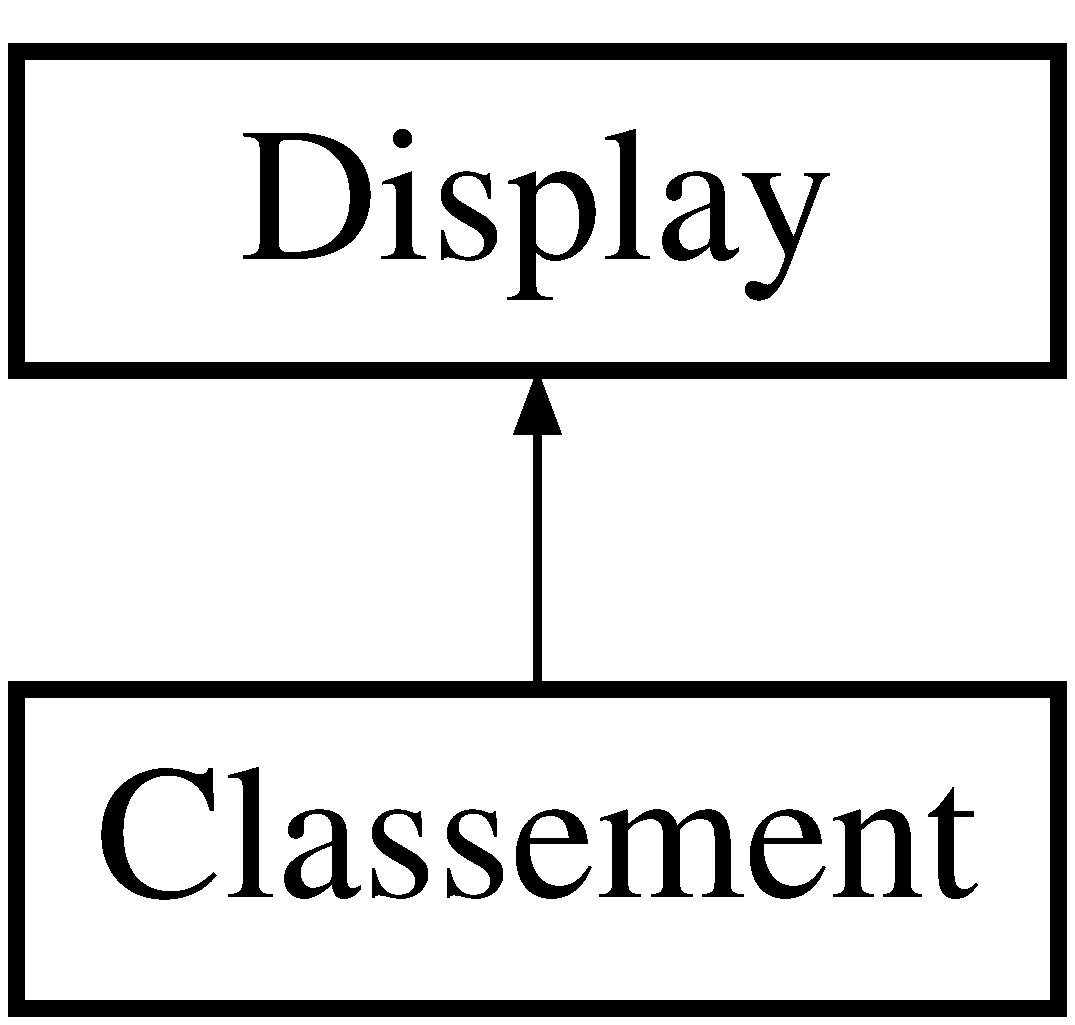
\includegraphics[height=2.000000cm]{classClassement}
\end{center}
\end{figure}
\subsection*{Membres hérités additionnels}


La documentation de cette classe a été générée à partir du fichier suivant \+:\begin{DoxyCompactItemize}
\item 
client/\hyperlink{client_2Classement_8hpp}{Classement.\+hpp}\end{DoxyCompactItemize}

\hypertarget{classCLI}{}\section{Référence de la classe C\+L\+I}
\label{classCLI}\index{C\+L\+I@{C\+L\+I}}


{\ttfamily \#include $<$C\+L\+I.\+hpp$>$}

Graphe d\textquotesingle{}héritage de C\+L\+I\+:\begin{figure}[H]
\begin{center}
\leavevmode
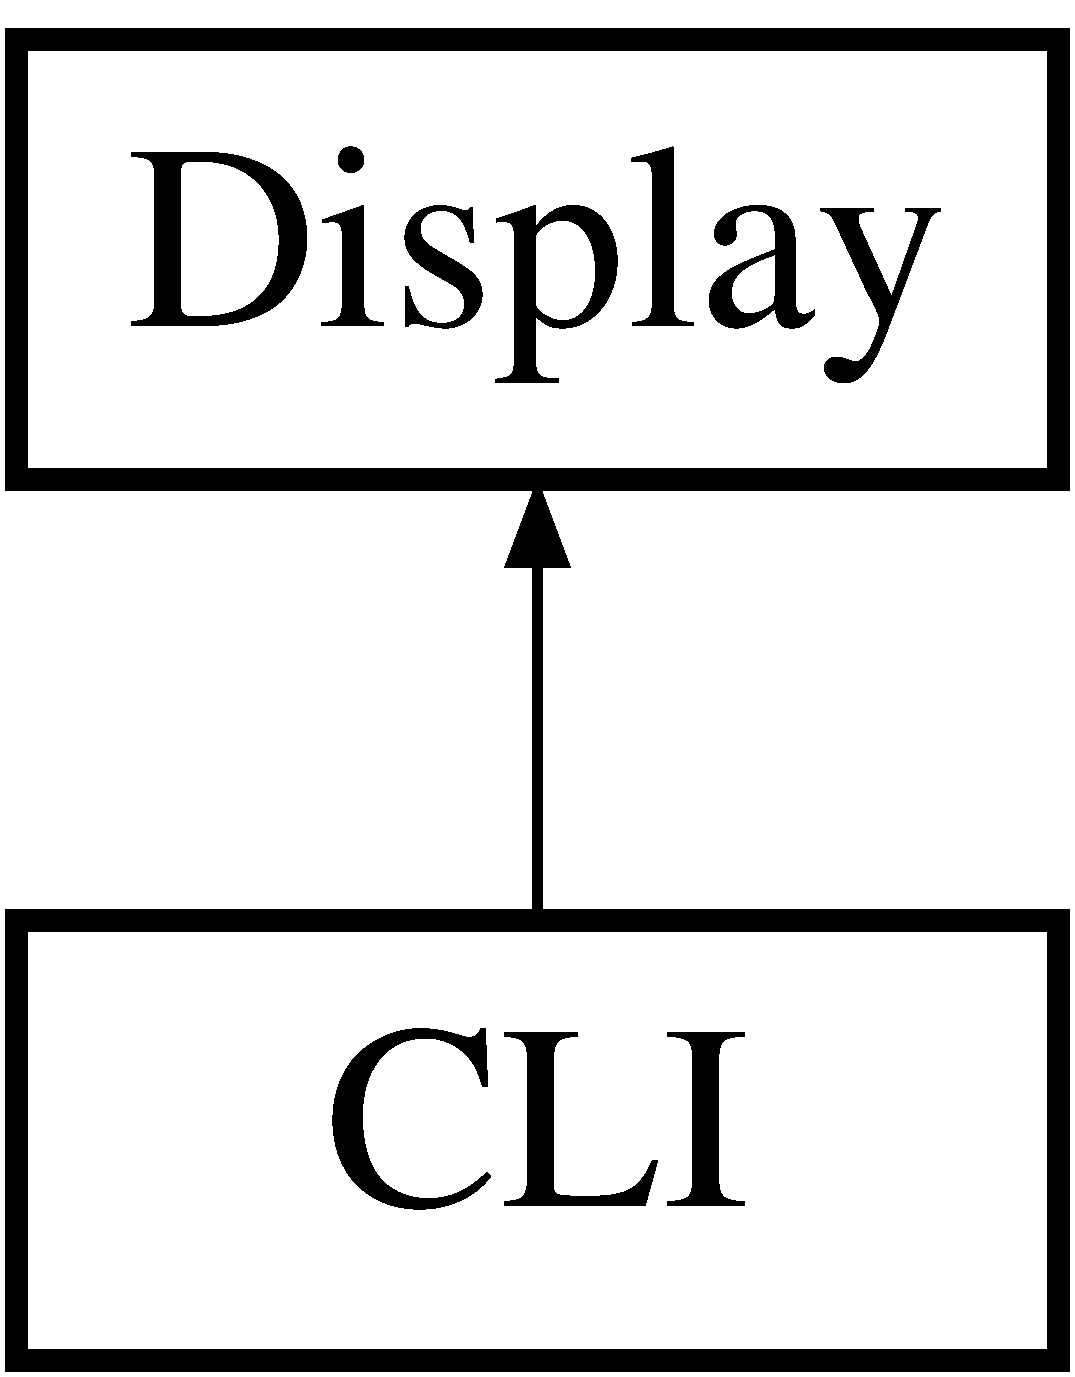
\includegraphics[height=2.000000cm]{classCLI}
\end{center}
\end{figure}
\subsection*{Fonctions membres publiques}
\begin{DoxyCompactItemize}
\item 
\hyperlink{classCLI_a1a5b0f7ec3b242c5c56e4745adbb391e}{C\+L\+I} ()
\item 
\hyperlink{classCLI_a9f59d57abf434f7161fcf3f61b725752}{$\sim$\+C\+L\+I} ()
\item 
void \hyperlink{classCLI_ae86da329edfde03f238c778481be2030}{display\+Fatal\+Error} (std\+::string)
\item 
void \hyperlink{classCLI_a6cf4acf9f7fa587cc49b892487c68f13}{display\+Login\+Prompt} ()
\item 
void \hyperlink{classCLI_abf864752edc73dba33fce8a0f06137c4}{display\+Login\+Result} (std\+::string)
\item 
void \hyperlink{classCLI_ac900759039333051b414c9002dd2100c}{valide\+Login} ()
\item 
void \hyperlink{classCLI_abcf6f643c8a94e0451b4b6d9ab9546c7}{display\+Main\+Window} ()
\item 
void \hyperlink{classCLI_a6b70a2b3d08d24f99826051c56a786e6}{display\+Friends\+Window} ()
\item 
void \hyperlink{classCLI_af20da7ff64f241fdd3659b66ffacedd4}{display\+Collection\+Window} ()
\item 
void \hyperlink{classCLI_a166fe45276733200e237c0d9cce3f801}{display\+Deck\+Window} ()
\item 
void \hyperlink{classCLI_ab6c8531d0ab6d343936a83edbb14703c}{display\+Wait} ()
\item 
void \hyperlink{classCLI_acef2afe60b53453ebf7ed52f4f06621e}{display\+Game} ()
\item 
void \hyperlink{classCLI_a2606c83484b8d0fa1fb6ea9ac2fe07de}{focus\+Tchat} ()
\end{DoxyCompactItemize}


\subsection{Documentation des constructeurs et destructeur}
\hypertarget{classCLI_a1a5b0f7ec3b242c5c56e4745adbb391e}{}\index{C\+L\+I@{C\+L\+I}!C\+L\+I@{C\+L\+I}}
\index{C\+L\+I@{C\+L\+I}!C\+L\+I@{C\+L\+I}}
\subsubsection[{C\+L\+I()}]{\setlength{\rightskip}{0pt plus 5cm}C\+L\+I\+::\+C\+L\+I (
\begin{DoxyParamCaption}
{}
\end{DoxyParamCaption}
)}\label{classCLI_a1a5b0f7ec3b242c5c56e4745adbb391e}
\hypertarget{classCLI_a9f59d57abf434f7161fcf3f61b725752}{}\index{C\+L\+I@{C\+L\+I}!````~C\+L\+I@{$\sim$\+C\+L\+I}}
\index{````~C\+L\+I@{$\sim$\+C\+L\+I}!C\+L\+I@{C\+L\+I}}
\subsubsection[{$\sim$\+C\+L\+I()}]{\setlength{\rightskip}{0pt plus 5cm}C\+L\+I\+::$\sim$\+C\+L\+I (
\begin{DoxyParamCaption}
{}
\end{DoxyParamCaption}
)}\label{classCLI_a9f59d57abf434f7161fcf3f61b725752}


\subsection{Documentation des fonctions membres}
\hypertarget{classCLI_af20da7ff64f241fdd3659b66ffacedd4}{}\index{C\+L\+I@{C\+L\+I}!display\+Collection\+Window@{display\+Collection\+Window}}
\index{display\+Collection\+Window@{display\+Collection\+Window}!C\+L\+I@{C\+L\+I}}
\subsubsection[{display\+Collection\+Window()}]{\setlength{\rightskip}{0pt plus 5cm}void C\+L\+I\+::display\+Collection\+Window (
\begin{DoxyParamCaption}
{}
\end{DoxyParamCaption}
)\hspace{0.3cm}{\ttfamily [virtual]}}\label{classCLI_af20da7ff64f241fdd3659b66ffacedd4}


Implémente \hyperlink{classDisplay_afb3efa4573ae41c513df30ba4c2691c0}{Display}.

\hypertarget{classCLI_a166fe45276733200e237c0d9cce3f801}{}\index{C\+L\+I@{C\+L\+I}!display\+Deck\+Window@{display\+Deck\+Window}}
\index{display\+Deck\+Window@{display\+Deck\+Window}!C\+L\+I@{C\+L\+I}}
\subsubsection[{display\+Deck\+Window()}]{\setlength{\rightskip}{0pt plus 5cm}void C\+L\+I\+::display\+Deck\+Window (
\begin{DoxyParamCaption}
{}
\end{DoxyParamCaption}
)\hspace{0.3cm}{\ttfamily [virtual]}}\label{classCLI_a166fe45276733200e237c0d9cce3f801}


Implémente \hyperlink{classDisplay_adbf8168f368a98a4c7797519e9b39948}{Display}.

\hypertarget{classCLI_ae86da329edfde03f238c778481be2030}{}\index{C\+L\+I@{C\+L\+I}!display\+Fatal\+Error@{display\+Fatal\+Error}}
\index{display\+Fatal\+Error@{display\+Fatal\+Error}!C\+L\+I@{C\+L\+I}}
\subsubsection[{display\+Fatal\+Error(std\+::string)}]{\setlength{\rightskip}{0pt plus 5cm}void C\+L\+I\+::display\+Fatal\+Error (
\begin{DoxyParamCaption}
\item[{std\+::string}]{error}
\end{DoxyParamCaption}
)\hspace{0.3cm}{\ttfamily [virtual]}}\label{classCLI_ae86da329edfde03f238c778481be2030}


Implémente \hyperlink{classDisplay_a9d41e789d52a29d773d7acddd9f01172}{Display}.

\hypertarget{classCLI_a6b70a2b3d08d24f99826051c56a786e6}{}\index{C\+L\+I@{C\+L\+I}!display\+Friends\+Window@{display\+Friends\+Window}}
\index{display\+Friends\+Window@{display\+Friends\+Window}!C\+L\+I@{C\+L\+I}}
\subsubsection[{display\+Friends\+Window()}]{\setlength{\rightskip}{0pt plus 5cm}void C\+L\+I\+::display\+Friends\+Window (
\begin{DoxyParamCaption}
{}
\end{DoxyParamCaption}
)\hspace{0.3cm}{\ttfamily [virtual]}}\label{classCLI_a6b70a2b3d08d24f99826051c56a786e6}


Implémente \hyperlink{classDisplay_ae80aee2a7bd67135e1756ba439946f8f}{Display}.

\hypertarget{classCLI_acef2afe60b53453ebf7ed52f4f06621e}{}\index{C\+L\+I@{C\+L\+I}!display\+Game@{display\+Game}}
\index{display\+Game@{display\+Game}!C\+L\+I@{C\+L\+I}}
\subsubsection[{display\+Game()}]{\setlength{\rightskip}{0pt plus 5cm}void C\+L\+I\+::display\+Game (
\begin{DoxyParamCaption}
{}
\end{DoxyParamCaption}
)\hspace{0.3cm}{\ttfamily [virtual]}}\label{classCLI_acef2afe60b53453ebf7ed52f4f06621e}


Implémente \hyperlink{classDisplay_af3d6e09060fc88351d0c0bf3d349770c}{Display}.

\hypertarget{classCLI_a6cf4acf9f7fa587cc49b892487c68f13}{}\index{C\+L\+I@{C\+L\+I}!display\+Login\+Prompt@{display\+Login\+Prompt}}
\index{display\+Login\+Prompt@{display\+Login\+Prompt}!C\+L\+I@{C\+L\+I}}
\subsubsection[{display\+Login\+Prompt()}]{\setlength{\rightskip}{0pt plus 5cm}void C\+L\+I\+::display\+Login\+Prompt (
\begin{DoxyParamCaption}
{}
\end{DoxyParamCaption}
)\hspace{0.3cm}{\ttfamily [virtual]}}\label{classCLI_a6cf4acf9f7fa587cc49b892487c68f13}


Implémente \hyperlink{classDisplay_a55719ab539ee6cc803d9de74b05f8e38}{Display}.

\hypertarget{classCLI_abf864752edc73dba33fce8a0f06137c4}{}\index{C\+L\+I@{C\+L\+I}!display\+Login\+Result@{display\+Login\+Result}}
\index{display\+Login\+Result@{display\+Login\+Result}!C\+L\+I@{C\+L\+I}}
\subsubsection[{display\+Login\+Result(std\+::string)}]{\setlength{\rightskip}{0pt plus 5cm}void C\+L\+I\+::display\+Login\+Result (
\begin{DoxyParamCaption}
\item[{std\+::string}]{error\+Message}
\end{DoxyParamCaption}
)\hspace{0.3cm}{\ttfamily [virtual]}}\label{classCLI_abf864752edc73dba33fce8a0f06137c4}


Implémente \hyperlink{classDisplay_ac4cc71c734feea0099bbeae89e6d2f1c}{Display}.

\hypertarget{classCLI_abcf6f643c8a94e0451b4b6d9ab9546c7}{}\index{C\+L\+I@{C\+L\+I}!display\+Main\+Window@{display\+Main\+Window}}
\index{display\+Main\+Window@{display\+Main\+Window}!C\+L\+I@{C\+L\+I}}
\subsubsection[{display\+Main\+Window()}]{\setlength{\rightskip}{0pt plus 5cm}void C\+L\+I\+::display\+Main\+Window (
\begin{DoxyParamCaption}
{}
\end{DoxyParamCaption}
)\hspace{0.3cm}{\ttfamily [virtual]}}\label{classCLI_abcf6f643c8a94e0451b4b6d9ab9546c7}


Implémente \hyperlink{classDisplay_a88a6e0ccafb0ef286149a9ab4ffb28ad}{Display}.

\hypertarget{classCLI_ab6c8531d0ab6d343936a83edbb14703c}{}\index{C\+L\+I@{C\+L\+I}!display\+Wait@{display\+Wait}}
\index{display\+Wait@{display\+Wait}!C\+L\+I@{C\+L\+I}}
\subsubsection[{display\+Wait()}]{\setlength{\rightskip}{0pt plus 5cm}void C\+L\+I\+::display\+Wait (
\begin{DoxyParamCaption}
{}
\end{DoxyParamCaption}
)\hspace{0.3cm}{\ttfamily [virtual]}}\label{classCLI_ab6c8531d0ab6d343936a83edbb14703c}


Implémente \hyperlink{classDisplay_ae3bff36aaa0be0e78b2df88c9b326138}{Display}.

\hypertarget{classCLI_a2606c83484b8d0fa1fb6ea9ac2fe07de}{}\index{C\+L\+I@{C\+L\+I}!focus\+Tchat@{focus\+Tchat}}
\index{focus\+Tchat@{focus\+Tchat}!C\+L\+I@{C\+L\+I}}
\subsubsection[{focus\+Tchat()}]{\setlength{\rightskip}{0pt plus 5cm}void C\+L\+I\+::focus\+Tchat (
\begin{DoxyParamCaption}
{}
\end{DoxyParamCaption}
)\hspace{0.3cm}{\ttfamily [virtual]}}\label{classCLI_a2606c83484b8d0fa1fb6ea9ac2fe07de}


Implémente \hyperlink{classDisplay_a66a03431e0f33d30d914b7b3decc0103}{Display}.

\hypertarget{classCLI_ac900759039333051b414c9002dd2100c}{}\index{C\+L\+I@{C\+L\+I}!valide\+Login@{valide\+Login}}
\index{valide\+Login@{valide\+Login}!C\+L\+I@{C\+L\+I}}
\subsubsection[{valide\+Login()}]{\setlength{\rightskip}{0pt plus 5cm}void C\+L\+I\+::valide\+Login (
\begin{DoxyParamCaption}
{}
\end{DoxyParamCaption}
)\hspace{0.3cm}{\ttfamily [virtual]}}\label{classCLI_ac900759039333051b414c9002dd2100c}


Implémente \hyperlink{classDisplay_a93154cf71b945b6ce3ef959a306629f2}{Display}.



La documentation de cette classe a été générée à partir des fichiers suivants \+:\begin{DoxyCompactItemize}
\item 
client/\hyperlink{CLI_8hpp}{C\+L\+I.\+hpp}\item 
client/\hyperlink{CLI_8cpp}{C\+L\+I.\+cpp}\end{DoxyCompactItemize}

\hypertarget{classCollection}{}\section{Référence de la classe Collection}
\label{classCollection}\index{Collection@{Collection}}


{\ttfamily \#include $<$Collection.\+hpp$>$}

Graphe d\textquotesingle{}héritage de Collection\+:\begin{figure}[H]
\begin{center}
\leavevmode
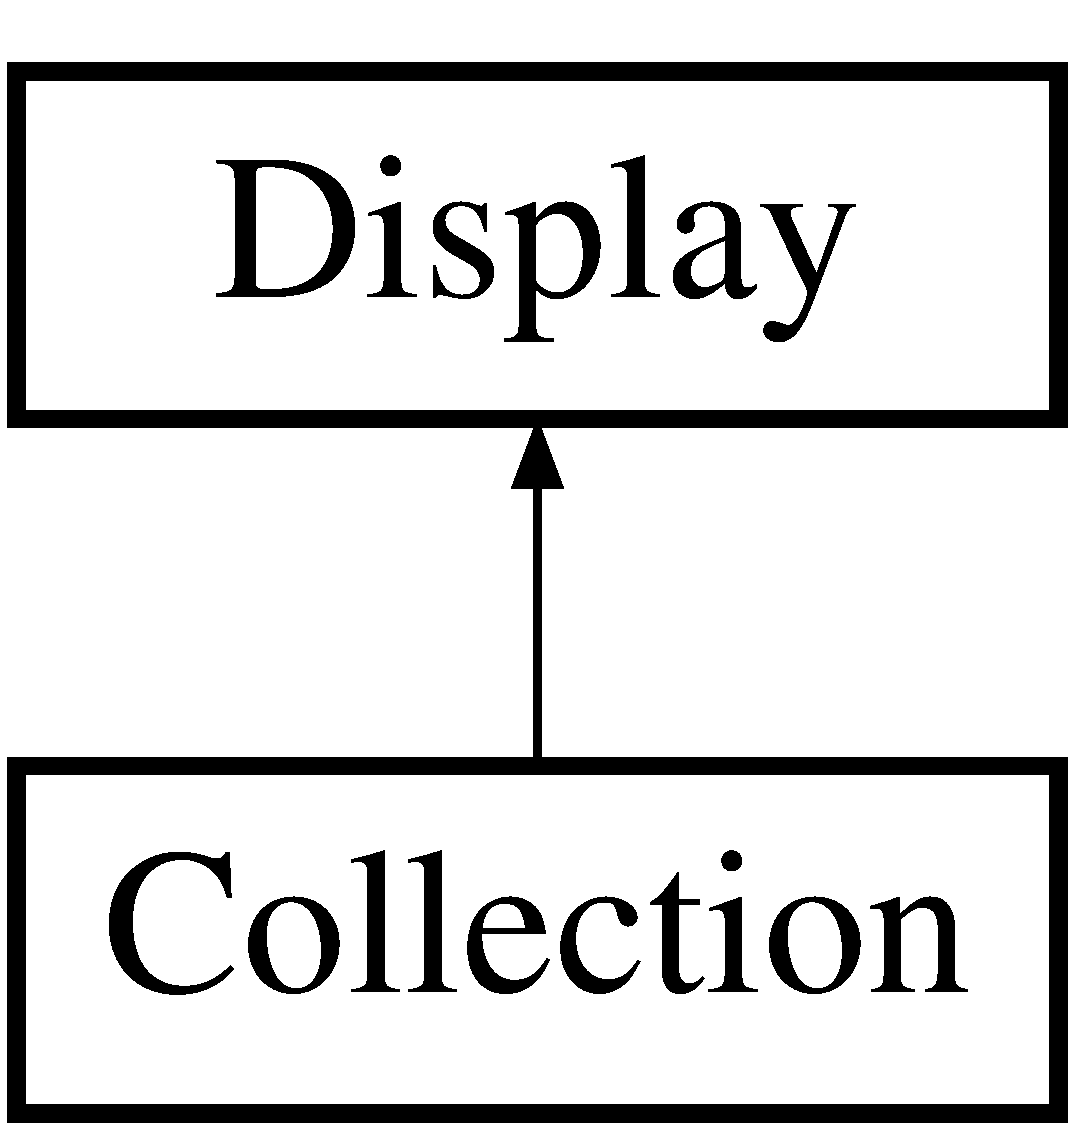
\includegraphics[height=2.000000cm]{classCollection}
\end{center}
\end{figure}
\subsection*{Fonctions membres publiques}
\begin{DoxyCompactItemize}
\item 
\hyperlink{classCollection_a5a47d67f2f24553ea9adde4f4f286dc6}{Collection} ()=default
\item 
\hyperlink{classCollection_ab635b340b56740374abd52368087be0b}{Collection} (std\+::vector$<$ \hyperlink{classCard}{Card} $\ast$ $>$)
\item 
\hyperlink{classCollection_a68b48e6494b0a52b1c873c5fd8420007}{Collection} (std\+::vector$<$ unsigned $>$)
\item 
\hyperlink{classCollection_ac6947d19970d090b545eef22c101087d}{Collection} (const \hyperlink{classCollection}{Collection} \&)=default
\item 
\hyperlink{classCollection}{Collection} \& \hyperlink{classCollection_afdc6e54deac9226fda136ca4bb8a97a1}{operator=} (const \hyperlink{classCollection}{Collection} \&)=default
\item 
virtual \hyperlink{Error_8hpp_a2c3e4bb40f36b262a5214e2da2bca9c5}{Error} \hyperlink{classCollection_a430b67b03697286c696b9972de4b7b4b}{add\+Card} (\hyperlink{classCard}{Card} $\ast$)
\item 
virtual \hyperlink{Error_8hpp_a2c3e4bb40f36b262a5214e2da2bca9c5}{Error} \hyperlink{classCollection_a580daf9636192634d949951ceffba096}{add\+Card} (int card\+Id)
\item 
void \hyperlink{classCollection_ae7ee9c1b7e8619d2cf851e5c0dbd81b6}{remove\+Card} (int i)
\item 
void \hyperlink{classCollection_a2020d4aef89fd4c70141ce2e2d061ae9}{remove\+Card} (\hyperlink{classCard}{Card} $\ast$)
\item 
void \hyperlink{classCollection_a633b047916ca73598b08c019ffe6c4a5}{remove\+Card\+Id} (int card\+Id)
\item 
int \hyperlink{classCollection_a9bd74b104abcc47257564044be71a6b2}{index\+Of\+Card} (int card\+Id)
\item 
int \hyperlink{classCollection_aa7acabbd00d04898ffefce407645142e}{get\+Card\+Index} (\hyperlink{classCard}{Card} $\ast$)
\item 
\hyperlink{classCard}{Card} $\ast$ \hyperlink{classCollection_aced95e3b1de7bebeb22d9cb1d36d483b}{get\+Card\+On\+Index} (const unsigned index)
\item 
std\+::vector$<$ unsigned $>$ \hyperlink{classCollection_a1eaec13063d083a49ed9c26a4105d370}{get\+Cards\+Id} () const 
\item 
virtual \hyperlink{classCollection_ac7fe8e15953eee4ba235ee7ebc4ffc5b}{$\sim$\+Collection} ()=default
\end{DoxyCompactItemize}
\subsection*{Attributs protégés}
\begin{DoxyCompactItemize}
\item 
std\+::vector$<$ \hyperlink{classCard}{Card} $\ast$ $>$ \hyperlink{classCollection_aebfdc5b0559ab8a0c350a24c9d24f564}{\+\_\+list\+Card}
\end{DoxyCompactItemize}


\subsection{Documentation des constructeurs et destructeur}
\hypertarget{classCollection_a5a47d67f2f24553ea9adde4f4f286dc6}{}\index{Collection@{Collection}!Collection@{Collection}}
\index{Collection@{Collection}!Collection@{Collection}}
\subsubsection[{Collection()=default}]{\setlength{\rightskip}{0pt plus 5cm}Collection\+::\+Collection (
\begin{DoxyParamCaption}
{}
\end{DoxyParamCaption}
)\hspace{0.3cm}{\ttfamily [default]}}\label{classCollection_a5a47d67f2f24553ea9adde4f4f286dc6}
\hypertarget{classCollection_ab635b340b56740374abd52368087be0b}{}\index{Collection@{Collection}!Collection@{Collection}}
\index{Collection@{Collection}!Collection@{Collection}}
\subsubsection[{Collection(std\+::vector$<$ Card $\ast$ $>$)}]{\setlength{\rightskip}{0pt plus 5cm}Collection\+::\+Collection (
\begin{DoxyParamCaption}
\item[{std\+::vector$<$ {\bf Card} $\ast$ $>$}]{list\+Card}
\end{DoxyParamCaption}
)}\label{classCollection_ab635b340b56740374abd52368087be0b}
Constructor


\begin{DoxyParams}{Paramètres}
{\em list\+Card} & list of card \\
\hline
\end{DoxyParams}
\hypertarget{classCollection_a68b48e6494b0a52b1c873c5fd8420007}{}\index{Collection@{Collection}!Collection@{Collection}}
\index{Collection@{Collection}!Collection@{Collection}}
\subsubsection[{Collection(std\+::vector$<$ unsigned $>$)}]{\setlength{\rightskip}{0pt plus 5cm}Collection\+::\+Collection (
\begin{DoxyParamCaption}
\item[{std\+::vector$<$ unsigned $>$}]{list\+Id\+Card}
\end{DoxyParamCaption}
)}\label{classCollection_a68b48e6494b0a52b1c873c5fd8420007}
Constructor


\begin{DoxyParams}{Paramètres}
{\em list\+Id\+Card} & the list of card I\+D \\
\hline
\end{DoxyParams}
\hypertarget{classCollection_ac6947d19970d090b545eef22c101087d}{}\index{Collection@{Collection}!Collection@{Collection}}
\index{Collection@{Collection}!Collection@{Collection}}
\subsubsection[{Collection(const Collection \&)=default}]{\setlength{\rightskip}{0pt plus 5cm}Collection\+::\+Collection (
\begin{DoxyParamCaption}
\item[{const {\bf Collection} \&}]{}
\end{DoxyParamCaption}
)\hspace{0.3cm}{\ttfamily [default]}}\label{classCollection_ac6947d19970d090b545eef22c101087d}
\hypertarget{classCollection_ac7fe8e15953eee4ba235ee7ebc4ffc5b}{}\index{Collection@{Collection}!````~Collection@{$\sim$\+Collection}}
\index{````~Collection@{$\sim$\+Collection}!Collection@{Collection}}
\subsubsection[{$\sim$\+Collection()=default}]{\setlength{\rightskip}{0pt plus 5cm}virtual Collection\+::$\sim$\+Collection (
\begin{DoxyParamCaption}
{}
\end{DoxyParamCaption}
)\hspace{0.3cm}{\ttfamily [virtual]}, {\ttfamily [default]}}\label{classCollection_ac7fe8e15953eee4ba235ee7ebc4ffc5b}


\subsection{Documentation des fonctions membres}
\hypertarget{classCollection_a430b67b03697286c696b9972de4b7b4b}{}\index{Collection@{Collection}!add\+Card@{add\+Card}}
\index{add\+Card@{add\+Card}!Collection@{Collection}}
\subsubsection[{add\+Card(\+Card $\ast$)}]{\setlength{\rightskip}{0pt plus 5cm}{\bf Error} Collection\+::add\+Card (
\begin{DoxyParamCaption}
\item[{{\bf Card} $\ast$}]{card}
\end{DoxyParamCaption}
)\hspace{0.3cm}{\ttfamily [virtual]}}\label{classCollection_a430b67b03697286c696b9972de4b7b4b}
Add a \hyperlink{classCard}{Card} to the collection


\begin{DoxyParams}{Paramètres}
{\em card} & the card to add \\
\hline
\end{DoxyParams}
\begin{DoxyReturn}{Renvoie}
True if we can add \hyperlink{classCard}{Card} (false if there is more than two cards the same) 
\end{DoxyReturn}


Réimplémentée dans \hyperlink{classDeck_a741aa3330dc4912beb69c962e74df507}{Deck}.

\hypertarget{classCollection_a580daf9636192634d949951ceffba096}{}\index{Collection@{Collection}!add\+Card@{add\+Card}}
\index{add\+Card@{add\+Card}!Collection@{Collection}}
\subsubsection[{add\+Card(int card\+Id)}]{\setlength{\rightskip}{0pt plus 5cm}{\bf Error} Collection\+::add\+Card (
\begin{DoxyParamCaption}
\item[{int}]{card\+Id}
\end{DoxyParamCaption}
)\hspace{0.3cm}{\ttfamily [virtual]}}\label{classCollection_a580daf9636192634d949951ceffba096}
Add a \hyperlink{classCard}{Card} to the collection


\begin{DoxyParams}{Paramètres}
{\em card\+Id} & the id of the card \\
\hline
\end{DoxyParams}
\begin{DoxyReturn}{Renvoie}
True if we can add \hyperlink{classCard}{Card} (false if there is more than two cards the same) 
\end{DoxyReturn}


Réimplémentée dans \hyperlink{classDeck_a5c18872420a1969dba61ee3eca320aa7}{Deck}.

\hypertarget{classCollection_aa7acabbd00d04898ffefce407645142e}{}\index{Collection@{Collection}!get\+Card\+Index@{get\+Card\+Index}}
\index{get\+Card\+Index@{get\+Card\+Index}!Collection@{Collection}}
\subsubsection[{get\+Card\+Index(\+Card $\ast$)}]{\setlength{\rightskip}{0pt plus 5cm}int Collection\+::get\+Card\+Index (
\begin{DoxyParamCaption}
\item[{{\bf Card} $\ast$}]{card}
\end{DoxyParamCaption}
)}\label{classCollection_aa7acabbd00d04898ffefce407645142e}
Get the index of one card


\begin{DoxyParams}{Paramètres}
{\em card} & \\
\hline
\end{DoxyParams}
\begin{DoxyReturn}{Renvoie}
index or -\/1 if not found 
\end{DoxyReturn}
\hypertarget{classCollection_aced95e3b1de7bebeb22d9cb1d36d483b}{}\index{Collection@{Collection}!get\+Card\+On\+Index@{get\+Card\+On\+Index}}
\index{get\+Card\+On\+Index@{get\+Card\+On\+Index}!Collection@{Collection}}
\subsubsection[{get\+Card\+On\+Index(const unsigned index)}]{\setlength{\rightskip}{0pt plus 5cm}{\bf Card} $\ast$ Collection\+::get\+Card\+On\+Index (
\begin{DoxyParamCaption}
\item[{const unsigned}]{index}
\end{DoxyParamCaption}
)}\label{classCollection_aced95e3b1de7bebeb22d9cb1d36d483b}
Get the card on the specific index


\begin{DoxyParams}{Paramètres}
{\em index} & of the card \\
\hline
\end{DoxyParams}
\begin{DoxyReturn}{Renvoie}
the \hyperlink{classCard}{Card} at the specific index 
\end{DoxyReturn}
\hypertarget{classCollection_a1eaec13063d083a49ed9c26a4105d370}{}\index{Collection@{Collection}!get\+Cards\+Id@{get\+Cards\+Id}}
\index{get\+Cards\+Id@{get\+Cards\+Id}!Collection@{Collection}}
\subsubsection[{get\+Cards\+Id() const }]{\setlength{\rightskip}{0pt plus 5cm}std\+::vector$<$ unsigned $>$ Collection\+::get\+Cards\+Id (
\begin{DoxyParamCaption}
{}
\end{DoxyParamCaption}
) const}\label{classCollection_a1eaec13063d083a49ed9c26a4105d370}
\hypertarget{classCollection_a9bd74b104abcc47257564044be71a6b2}{}\index{Collection@{Collection}!index\+Of\+Card@{index\+Of\+Card}}
\index{index\+Of\+Card@{index\+Of\+Card}!Collection@{Collection}}
\subsubsection[{index\+Of\+Card(int card\+Id)}]{\setlength{\rightskip}{0pt plus 5cm}int Collection\+::index\+Of\+Card (
\begin{DoxyParamCaption}
\item[{int}]{card\+Id}
\end{DoxyParamCaption}
)}\label{classCollection_a9bd74b104abcc47257564044be71a6b2}
\hypertarget{classCollection_afdc6e54deac9226fda136ca4bb8a97a1}{}\index{Collection@{Collection}!operator=@{operator=}}
\index{operator=@{operator=}!Collection@{Collection}}
\subsubsection[{operator=(const Collection \&)=default}]{\setlength{\rightskip}{0pt plus 5cm}{\bf Collection}\& Collection\+::operator= (
\begin{DoxyParamCaption}
\item[{const {\bf Collection} \&}]{}
\end{DoxyParamCaption}
)\hspace{0.3cm}{\ttfamily [default]}}\label{classCollection_afdc6e54deac9226fda136ca4bb8a97a1}
\hypertarget{classCollection_ae7ee9c1b7e8619d2cf851e5c0dbd81b6}{}\index{Collection@{Collection}!remove\+Card@{remove\+Card}}
\index{remove\+Card@{remove\+Card}!Collection@{Collection}}
\subsubsection[{remove\+Card(int i)}]{\setlength{\rightskip}{0pt plus 5cm}void Collection\+::remove\+Card (
\begin{DoxyParamCaption}
\item[{int}]{i}
\end{DoxyParamCaption}
)}\label{classCollection_ae7ee9c1b7e8619d2cf851e5c0dbd81b6}
Remove a \hyperlink{classCard}{Card} on a specific position


\begin{DoxyParams}{Paramètres}
{\em i} & index of the card \\
\hline
\end{DoxyParams}
\hypertarget{classCollection_a2020d4aef89fd4c70141ce2e2d061ae9}{}\index{Collection@{Collection}!remove\+Card@{remove\+Card}}
\index{remove\+Card@{remove\+Card}!Collection@{Collection}}
\subsubsection[{remove\+Card(\+Card $\ast$)}]{\setlength{\rightskip}{0pt plus 5cm}void Collection\+::remove\+Card (
\begin{DoxyParamCaption}
\item[{{\bf Card} $\ast$}]{card}
\end{DoxyParamCaption}
)}\label{classCollection_a2020d4aef89fd4c70141ce2e2d061ae9}
Remove a \hyperlink{classCard}{Card} from the collection


\begin{DoxyParams}{Paramètres}
{\em card} & the card to remove \\
\hline
\end{DoxyParams}
\hypertarget{classCollection_a633b047916ca73598b08c019ffe6c4a5}{}\index{Collection@{Collection}!remove\+Card\+Id@{remove\+Card\+Id}}
\index{remove\+Card\+Id@{remove\+Card\+Id}!Collection@{Collection}}
\subsubsection[{remove\+Card\+Id(int card\+Id)}]{\setlength{\rightskip}{0pt plus 5cm}void Collection\+::remove\+Card\+Id (
\begin{DoxyParamCaption}
\item[{int}]{card\+Id}
\end{DoxyParamCaption}
)}\label{classCollection_a633b047916ca73598b08c019ffe6c4a5}
Remove a \hyperlink{classCard}{Card} from the collection


\begin{DoxyParams}{Paramètres}
{\em card\+Id} & the id of the card \\
\hline
\end{DoxyParams}


\subsection{Documentation des données membres}
\hypertarget{classCollection_aebfdc5b0559ab8a0c350a24c9d24f564}{}\index{Collection@{Collection}!\+\_\+list\+Card@{\+\_\+list\+Card}}
\index{\+\_\+list\+Card@{\+\_\+list\+Card}!Collection@{Collection}}
\subsubsection[{\+\_\+list\+Card}]{\setlength{\rightskip}{0pt plus 5cm}std\+::vector$<${\bf Card}$\ast$$>$ Collection\+::\+\_\+list\+Card\hspace{0.3cm}{\ttfamily [protected]}}\label{classCollection_aebfdc5b0559ab8a0c350a24c9d24f564}


La documentation de cette classe a été générée à partir des fichiers suivants \+:\begin{DoxyCompactItemize}
\item 
server/\hyperlink{Collection_8hpp}{Collection.\+hpp}\item 
server/\hyperlink{Collection_8cpp}{Collection.\+cpp}\end{DoxyCompactItemize}

\hypertarget{structPacket_1_1collectionListPacket}{}\section{Référence de la structure Packet\+:\+:collection\+List\+Packet}
\label{structPacket_1_1collectionListPacket}\index{Packet\+::collection\+List\+Packet@{Packet\+::collection\+List\+Packet}}


{\ttfamily \#include $<$Packet.\+hpp$>$}

\subsection*{Attributs publics}
\begin{DoxyCompactItemize}
\item 
int \hyperlink{structPacket_1_1collectionListPacket_af8e389e458f39647b120772359f4799d}{I\+D} = \hyperlink{classPacket_ae91c1d355e4c8f0bef5f893747473661a257c56805034a2a1288c8b627f7c4e42}{C\+O\+L\+L\+E\+C\+T\+I\+O\+N\+\_\+\+L\+I\+S\+T\+\_\+\+I\+D}
\item 
int \hyperlink{structPacket_1_1collectionListPacket_a7e5da725f1892d00962cd8526e4959d7}{size} = sizeof(int)$\ast$\hyperlink{Packet_8hpp_a6e39296d8aea63f64e88541e9ffadc56}{M\+A\+X\+\_\+\+C\+A\+R\+T\+E\+S}
\item 
int \hyperlink{structPacket_1_1collectionListPacket_a54a300514d3c4f5e37c721db03a2afb4}{cartes\+List} \mbox{[}\hyperlink{Packet_8hpp_a6e39296d8aea63f64e88541e9ffadc56}{M\+A\+X\+\_\+\+C\+A\+R\+T\+E\+S}\mbox{]}
\end{DoxyCompactItemize}


\subsection{Documentation des données membres}
\hypertarget{structPacket_1_1collectionListPacket_a54a300514d3c4f5e37c721db03a2afb4}{}\index{Packet\+::collection\+List\+Packet@{Packet\+::collection\+List\+Packet}!cartes\+List@{cartes\+List}}
\index{cartes\+List@{cartes\+List}!Packet\+::collection\+List\+Packet@{Packet\+::collection\+List\+Packet}}
\subsubsection[{cartes\+List}]{\setlength{\rightskip}{0pt plus 5cm}int Packet\+::collection\+List\+Packet\+::cartes\+List\mbox{[}{\bf M\+A\+X\+\_\+\+C\+A\+R\+T\+E\+S}\mbox{]}}\label{structPacket_1_1collectionListPacket_a54a300514d3c4f5e37c721db03a2afb4}
\hypertarget{structPacket_1_1collectionListPacket_af8e389e458f39647b120772359f4799d}{}\index{Packet\+::collection\+List\+Packet@{Packet\+::collection\+List\+Packet}!I\+D@{I\+D}}
\index{I\+D@{I\+D}!Packet\+::collection\+List\+Packet@{Packet\+::collection\+List\+Packet}}
\subsubsection[{I\+D}]{\setlength{\rightskip}{0pt plus 5cm}int Packet\+::collection\+List\+Packet\+::\+I\+D = {\bf C\+O\+L\+L\+E\+C\+T\+I\+O\+N\+\_\+\+L\+I\+S\+T\+\_\+\+I\+D}}\label{structPacket_1_1collectionListPacket_af8e389e458f39647b120772359f4799d}
\hypertarget{structPacket_1_1collectionListPacket_a7e5da725f1892d00962cd8526e4959d7}{}\index{Packet\+::collection\+List\+Packet@{Packet\+::collection\+List\+Packet}!size@{size}}
\index{size@{size}!Packet\+::collection\+List\+Packet@{Packet\+::collection\+List\+Packet}}
\subsubsection[{size}]{\setlength{\rightskip}{0pt plus 5cm}int Packet\+::collection\+List\+Packet\+::size = sizeof(int)$\ast${\bf M\+A\+X\+\_\+\+C\+A\+R\+T\+E\+S}}\label{structPacket_1_1collectionListPacket_a7e5da725f1892d00962cd8526e4959d7}


La documentation de cette structure a été générée à partir du fichier suivant \+:\begin{DoxyCompactItemize}
\item 
common/\hyperlink{Packet_8hpp}{Packet.\+hpp}\end{DoxyCompactItemize}

\hypertarget{classConnection}{}\section{Référence de la classe Connection}
\label{classConnection}\index{Connection@{Connection}}


{\ttfamily \#include $<$Connection.\+hpp$>$}

\subsection*{Fonctions membres publiques}
\begin{DoxyCompactItemize}
\item 
\hyperlink{classConnection_ab7b5c72eb0e2f7ce6f0e1f2c20b7389d}{Connection} (char $\ast$)
\item 
\hyperlink{classConnection_a2e4352edf667bea83001569e9da8a24d}{$\sim$\+Connection} ()
\item 
void \hyperlink{classConnection_acf311ea2f3df77851711daf40a07fc17}{send\+Packet} (\hyperlink{classPacket}{Packet} $\ast$, long unsigned int)
\item 
\hyperlink{classConnection_a9de94289ca6259f94ef6aeba3b134a77}{Connection} ()
\item 
\hyperlink{classConnection_a2e4352edf667bea83001569e9da8a24d}{$\sim$\+Connection} ()
\item 
void \hyperlink{classConnection_af5678fe6f97c6c7f1258cd0972652374}{main\+Loop} ()
\end{DoxyCompactItemize}


\subsection{Documentation des constructeurs et destructeur}
\hypertarget{classConnection_ab7b5c72eb0e2f7ce6f0e1f2c20b7389d}{}\index{Connection@{Connection}!Connection@{Connection}}
\index{Connection@{Connection}!Connection@{Connection}}
\subsubsection[{Connection(char $\ast$)}]{\setlength{\rightskip}{0pt plus 5cm}Connection\+::\+Connection (
\begin{DoxyParamCaption}
\item[{char $\ast$}]{host\+Name}
\end{DoxyParamCaption}
)}\label{classConnection_ab7b5c72eb0e2f7ce6f0e1f2c20b7389d}
\hypertarget{classConnection_a2e4352edf667bea83001569e9da8a24d}{}\index{Connection@{Connection}!````~Connection@{$\sim$\+Connection}}
\index{````~Connection@{$\sim$\+Connection}!Connection@{Connection}}
\subsubsection[{$\sim$\+Connection()}]{\setlength{\rightskip}{0pt plus 5cm}Connection\+::$\sim$\+Connection (
\begin{DoxyParamCaption}
{}
\end{DoxyParamCaption}
)}\label{classConnection_a2e4352edf667bea83001569e9da8a24d}
\hypertarget{classConnection_a9de94289ca6259f94ef6aeba3b134a77}{}\index{Connection@{Connection}!Connection@{Connection}}
\index{Connection@{Connection}!Connection@{Connection}}
\subsubsection[{Connection()}]{\setlength{\rightskip}{0pt plus 5cm}Connection\+::\+Connection (
\begin{DoxyParamCaption}
{}
\end{DoxyParamCaption}
)}\label{classConnection_a9de94289ca6259f94ef6aeba3b134a77}
\hypertarget{classConnection_a2e4352edf667bea83001569e9da8a24d}{}\index{Connection@{Connection}!````~Connection@{$\sim$\+Connection}}
\index{````~Connection@{$\sim$\+Connection}!Connection@{Connection}}
\subsubsection[{$\sim$\+Connection()}]{\setlength{\rightskip}{0pt plus 5cm}Connection\+::$\sim$\+Connection (
\begin{DoxyParamCaption}
{}
\end{DoxyParamCaption}
)}\label{classConnection_a2e4352edf667bea83001569e9da8a24d}


\subsection{Documentation des fonctions membres}
\hypertarget{classConnection_af5678fe6f97c6c7f1258cd0972652374}{}\index{Connection@{Connection}!main\+Loop@{main\+Loop}}
\index{main\+Loop@{main\+Loop}!Connection@{Connection}}
\subsubsection[{main\+Loop()}]{\setlength{\rightskip}{0pt plus 5cm}void Connection\+::main\+Loop (
\begin{DoxyParamCaption}
{}
\end{DoxyParamCaption}
)}\label{classConnection_af5678fe6f97c6c7f1258cd0972652374}
\hypertarget{classConnection_acf311ea2f3df77851711daf40a07fc17}{}\index{Connection@{Connection}!send\+Packet@{send\+Packet}}
\index{send\+Packet@{send\+Packet}!Connection@{Connection}}
\subsubsection[{send\+Packet(\+Packet $\ast$, long unsigned int)}]{\setlength{\rightskip}{0pt plus 5cm}void Connection\+::send\+Packet (
\begin{DoxyParamCaption}
\item[{{\bf Packet} $\ast$}]{packet, }
\item[{long unsigned int}]{size}
\end{DoxyParamCaption}
)}\label{classConnection_acf311ea2f3df77851711daf40a07fc17}


La documentation de cette classe a été générée à partir des fichiers suivants \+:\begin{DoxyCompactItemize}
\item 
client/\hyperlink{client_2Connection_8hpp}{Connection.\+hpp}\item 
client/\hyperlink{client_2Connection_8cpp}{Connection.\+cpp}\end{DoxyCompactItemize}

\hypertarget{structdataIGPlayer}{}\section{Référence de la structure data\+I\+G\+Player}
\label{structdataIGPlayer}\index{data\+I\+G\+Player@{data\+I\+G\+Player}}


{\ttfamily \#include $<$Player\+In\+Game.\+hpp$>$}

\subsection*{Attributs publics}
\begin{DoxyCompactItemize}
\item 
int \hyperlink{structdataIGPlayer_addf0349de6577e21e1697b0853f37afb}{player\+Heal}
\item 
int \hyperlink{structdataIGPlayer_a62d62c03941a981f96ae02098ae8d2e2}{energy}
\item 
int \hyperlink{structdataIGPlayer_a27dcb13892444b5fcfebe7d01d05141a}{max\+Energy}
\item 
int \hyperlink{structdataIGPlayer_ae0958559747cb2ebad4e6c7ba6095c3f}{limit\+Energy}
\item 
std\+::vector$<$ \hyperlink{classCard}{Card} $\ast$ $>$ \hyperlink{structdataIGPlayer_a7b7ae3550424bffaff4cba98fdd2e39b}{cards\+In\+Hand}
\item 
std\+::vector$<$ \hyperlink{classCardMonster}{Card\+Monster} $\ast$ $>$ \hyperlink{structdataIGPlayer_a32709b71453d54100f95fae5535c0cb5}{cards\+Placed}
\item 
bool \hyperlink{structdataIGPlayer_a42cbe10f46e1e6bbd514e624cf6e1526}{turn}
\end{DoxyCompactItemize}


\subsection{Documentation des données membres}
\hypertarget{structdataIGPlayer_a7b7ae3550424bffaff4cba98fdd2e39b}{}\index{data\+I\+G\+Player@{data\+I\+G\+Player}!cards\+In\+Hand@{cards\+In\+Hand}}
\index{cards\+In\+Hand@{cards\+In\+Hand}!data\+I\+G\+Player@{data\+I\+G\+Player}}
\subsubsection[{cards\+In\+Hand}]{\setlength{\rightskip}{0pt plus 5cm}std\+::vector$<${\bf Card}$\ast$$>$ data\+I\+G\+Player\+::cards\+In\+Hand}\label{structdataIGPlayer_a7b7ae3550424bffaff4cba98fdd2e39b}
\hypertarget{structdataIGPlayer_a32709b71453d54100f95fae5535c0cb5}{}\index{data\+I\+G\+Player@{data\+I\+G\+Player}!cards\+Placed@{cards\+Placed}}
\index{cards\+Placed@{cards\+Placed}!data\+I\+G\+Player@{data\+I\+G\+Player}}
\subsubsection[{cards\+Placed}]{\setlength{\rightskip}{0pt plus 5cm}std\+::vector$<${\bf Card\+Monster}$\ast$$>$ data\+I\+G\+Player\+::cards\+Placed}\label{structdataIGPlayer_a32709b71453d54100f95fae5535c0cb5}
\hypertarget{structdataIGPlayer_a62d62c03941a981f96ae02098ae8d2e2}{}\index{data\+I\+G\+Player@{data\+I\+G\+Player}!energy@{energy}}
\index{energy@{energy}!data\+I\+G\+Player@{data\+I\+G\+Player}}
\subsubsection[{energy}]{\setlength{\rightskip}{0pt plus 5cm}int data\+I\+G\+Player\+::energy}\label{structdataIGPlayer_a62d62c03941a981f96ae02098ae8d2e2}
\hypertarget{structdataIGPlayer_ae0958559747cb2ebad4e6c7ba6095c3f}{}\index{data\+I\+G\+Player@{data\+I\+G\+Player}!limit\+Energy@{limit\+Energy}}
\index{limit\+Energy@{limit\+Energy}!data\+I\+G\+Player@{data\+I\+G\+Player}}
\subsubsection[{limit\+Energy}]{\setlength{\rightskip}{0pt plus 5cm}int data\+I\+G\+Player\+::limit\+Energy}\label{structdataIGPlayer_ae0958559747cb2ebad4e6c7ba6095c3f}
\hypertarget{structdataIGPlayer_a27dcb13892444b5fcfebe7d01d05141a}{}\index{data\+I\+G\+Player@{data\+I\+G\+Player}!max\+Energy@{max\+Energy}}
\index{max\+Energy@{max\+Energy}!data\+I\+G\+Player@{data\+I\+G\+Player}}
\subsubsection[{max\+Energy}]{\setlength{\rightskip}{0pt plus 5cm}int data\+I\+G\+Player\+::max\+Energy}\label{structdataIGPlayer_a27dcb13892444b5fcfebe7d01d05141a}
\hypertarget{structdataIGPlayer_addf0349de6577e21e1697b0853f37afb}{}\index{data\+I\+G\+Player@{data\+I\+G\+Player}!player\+Heal@{player\+Heal}}
\index{player\+Heal@{player\+Heal}!data\+I\+G\+Player@{data\+I\+G\+Player}}
\subsubsection[{player\+Heal}]{\setlength{\rightskip}{0pt plus 5cm}int data\+I\+G\+Player\+::player\+Heal}\label{structdataIGPlayer_addf0349de6577e21e1697b0853f37afb}
\hypertarget{structdataIGPlayer_a42cbe10f46e1e6bbd514e624cf6e1526}{}\index{data\+I\+G\+Player@{data\+I\+G\+Player}!turn@{turn}}
\index{turn@{turn}!data\+I\+G\+Player@{data\+I\+G\+Player}}
\subsubsection[{turn}]{\setlength{\rightskip}{0pt plus 5cm}bool data\+I\+G\+Player\+::turn}\label{structdataIGPlayer_a42cbe10f46e1e6bbd514e624cf6e1526}


La documentation de cette structure a été générée à partir du fichier suivant \+:\begin{DoxyCompactItemize}
\item 
server/\hyperlink{PlayerInGame_8hpp}{Player\+In\+Game.\+hpp}\end{DoxyCompactItemize}

\hypertarget{classDeck}{}\section{Référence de la classe Deck}
\label{classDeck}\index{Deck@{Deck}}


{\ttfamily \#include $<$Deck.\+hpp$>$}

Graphe d\textquotesingle{}héritage de Deck\+:\begin{figure}[H]
\begin{center}
\leavevmode
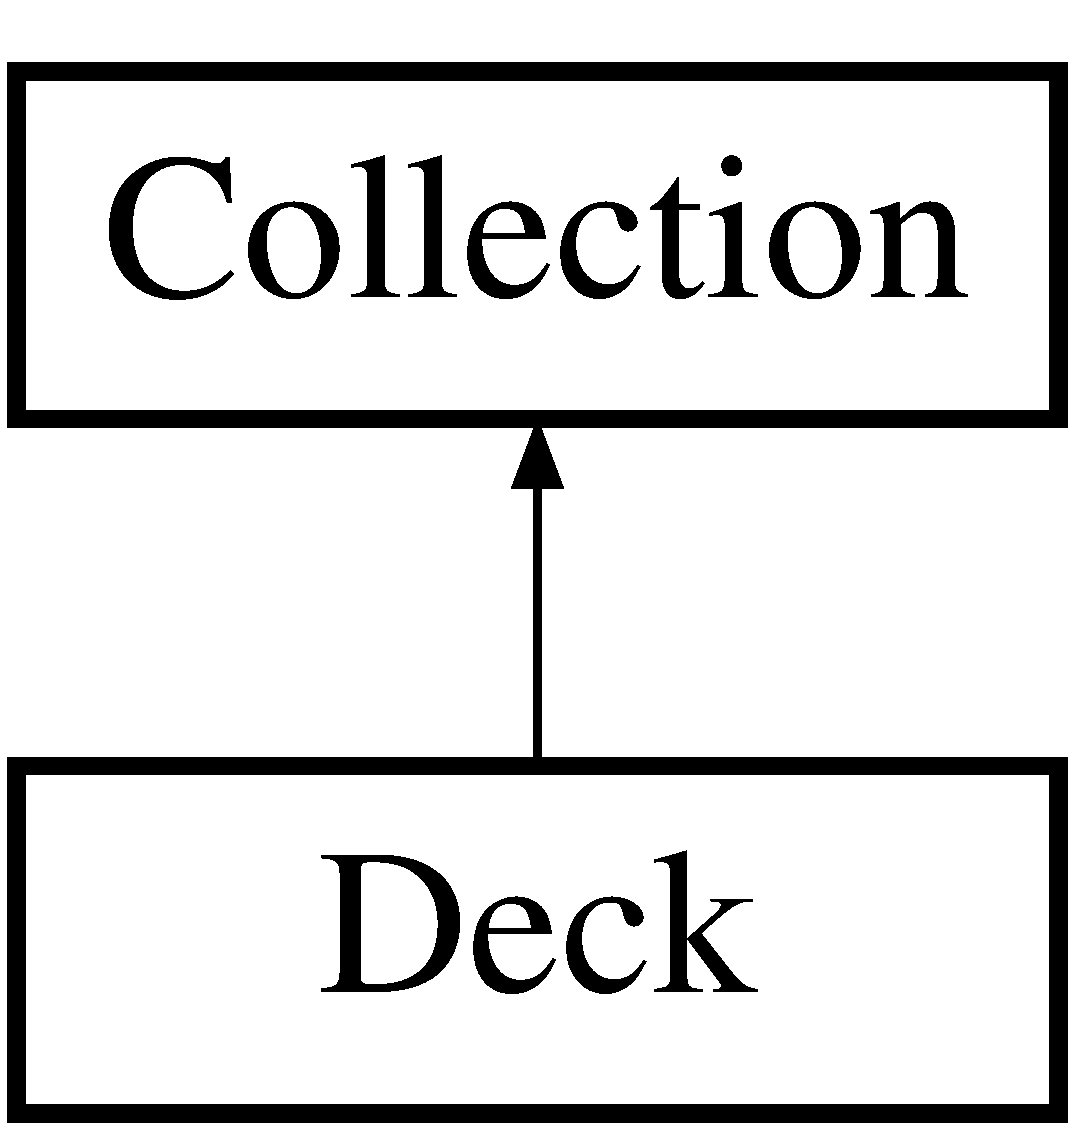
\includegraphics[height=2.000000cm]{classDeck}
\end{center}
\end{figure}
\subsection*{Fonctions membres publiques}
\begin{DoxyCompactItemize}
\item 
\hyperlink{classDeck_ab7f2fc685f721ab93884d04826db1de0}{Deck} (std\+::string name, std\+::vector$<$ \hyperlink{classCard}{Card} $\ast$ $>$ list\+Card)
\item 
\hyperlink{classDeck_a34d860bcef590d58850606102623da07}{Deck} (std\+::string name, std\+::vector$<$ unsigned $>$ list\+Card)
\item 
\hyperlink{classDeck_a11233381fd5ea0b0b4e6288048f146fa}{Deck} (const \hyperlink{classDeck}{Deck} \&)
\item 
\hyperlink{classDeck}{Deck} \& \hyperlink{classDeck_ac3d2eaa856438ec34f898821e7e76a6d}{operator=} (const \hyperlink{classDeck}{Deck} \&)=default
\item 
std\+::string \hyperlink{classDeck_aaa3db432259e3fd24431e0cef7a83ec0}{get\+Name} ()
\item 
bool \hyperlink{classDeck_a66cfb2d1adfb6b0b94ed25c8f5ca29f9}{is\+Valide} ()
\item 
\hyperlink{classCard}{Card} $\ast$ \hyperlink{classDeck_a910d3c6c7a83168fd7f2485778d5bfe0}{pickup} ()
\item 
virtual \hyperlink{Error_8hpp_a2c3e4bb40f36b262a5214e2da2bca9c5}{Error} \hyperlink{classDeck_a741aa3330dc4912beb69c962e74df507}{add\+Card} (\hyperlink{classCard}{Card} $\ast$card) override
\item 
virtual \hyperlink{Error_8hpp_a2c3e4bb40f36b262a5214e2da2bca9c5}{Error} \hyperlink{classDeck_a5c18872420a1969dba61ee3eca320aa7}{add\+Card} (int card\+Id) override
\item 
bool \hyperlink{classDeck_a360cf67965cd28b8bdda3ec932ae3296}{delete\+Deck} (\hyperlink{classPlayerInGame}{Player\+In\+Game} $\ast$)
\item 
\hyperlink{classDeck}{Deck} $\ast$ \hyperlink{classDeck_ab216a347587d7afe42adecb58a42fcbb}{copy\+Deck} ()
\end{DoxyCompactItemize}
\subsection*{Fonctions membres publiques statiques}
\begin{DoxyCompactItemize}
\item 
static \hyperlink{classDeck}{Deck} $\ast$ \hyperlink{classDeck_ae5ff1528ce1d9752c2ddb928de943d3e}{get\+Deck} (std\+::string, std\+::vector$<$ \hyperlink{classDeck}{Deck} $\ast$ $>$)
\end{DoxyCompactItemize}


\subsection{Description détaillée}
A deck is a list of 20 Cards (or less) 

\subsection{Documentation des constructeurs et destructeur}
\hypertarget{classDeck_ab7f2fc685f721ab93884d04826db1de0}{}\index{Deck@{Deck}!Deck@{Deck}}
\index{Deck@{Deck}!Deck@{Deck}}
\subsubsection[{Deck(std\+::string name, std\+::vector$<$ Card $\ast$ $>$ list\+Card)}]{\setlength{\rightskip}{0pt plus 5cm}Deck\+::\+Deck (
\begin{DoxyParamCaption}
\item[{std\+::string}]{name, }
\item[{std\+::vector$<$ {\bf Card} $\ast$ $>$}]{list\+Card}
\end{DoxyParamCaption}
)}\label{classDeck_ab7f2fc685f721ab93884d04826db1de0}
Constructor


\begin{DoxyParams}{Paramètres}
{\em name} & of the deck \\
\hline
{\em list\+Card} & the must be add on deck \\
\hline
\end{DoxyParams}
\hypertarget{classDeck_a34d860bcef590d58850606102623da07}{}\index{Deck@{Deck}!Deck@{Deck}}
\index{Deck@{Deck}!Deck@{Deck}}
\subsubsection[{Deck(std\+::string name, std\+::vector$<$ unsigned $>$ list\+Card)}]{\setlength{\rightskip}{0pt plus 5cm}Deck\+::\+Deck (
\begin{DoxyParamCaption}
\item[{std\+::string}]{name, }
\item[{std\+::vector$<$ unsigned $>$}]{list\+Card}
\end{DoxyParamCaption}
)}\label{classDeck_a34d860bcef590d58850606102623da07}
Constructor


\begin{DoxyParams}{Paramètres}
{\em name} & of the deck \\
\hline
{\em list\+Card} & the must be add on deck \\
\hline
\end{DoxyParams}
\hypertarget{classDeck_a11233381fd5ea0b0b4e6288048f146fa}{}\index{Deck@{Deck}!Deck@{Deck}}
\index{Deck@{Deck}!Deck@{Deck}}
\subsubsection[{Deck(const Deck \&)}]{\setlength{\rightskip}{0pt plus 5cm}Deck\+::\+Deck (
\begin{DoxyParamCaption}
\item[{const {\bf Deck} \&}]{deck}
\end{DoxyParamCaption}
)}\label{classDeck_a11233381fd5ea0b0b4e6288048f146fa}
Copy Constructor


\begin{DoxyParams}{Paramètres}
{\em deck} & to copy \\
\hline
\end{DoxyParams}


\subsection{Documentation des fonctions membres}
\hypertarget{classDeck_a741aa3330dc4912beb69c962e74df507}{}\index{Deck@{Deck}!add\+Card@{add\+Card}}
\index{add\+Card@{add\+Card}!Deck@{Deck}}
\subsubsection[{add\+Card(\+Card $\ast$card) override}]{\setlength{\rightskip}{0pt plus 5cm}{\bf Error} Deck\+::add\+Card (
\begin{DoxyParamCaption}
\item[{{\bf Card} $\ast$}]{card}
\end{DoxyParamCaption}
)\hspace{0.3cm}{\ttfamily [override]}, {\ttfamily [virtual]}}\label{classDeck_a741aa3330dc4912beb69c962e74df507}
Adds a card in the deck


\begin{DoxyParams}{Paramètres}
{\em card} & the card to add \\
\hline
\end{DoxyParams}
\begin{DoxyReturn}{Renvoie}
Error and No\+Error if all is ok 
\end{DoxyReturn}


Réimplémentée à partir de \hyperlink{classCollection_a430b67b03697286c696b9972de4b7b4b}{Collection}.

\hypertarget{classDeck_a5c18872420a1969dba61ee3eca320aa7}{}\index{Deck@{Deck}!add\+Card@{add\+Card}}
\index{add\+Card@{add\+Card}!Deck@{Deck}}
\subsubsection[{add\+Card(int card\+Id) override}]{\setlength{\rightskip}{0pt plus 5cm}{\bf Error} Deck\+::add\+Card (
\begin{DoxyParamCaption}
\item[{int}]{card\+Id}
\end{DoxyParamCaption}
)\hspace{0.3cm}{\ttfamily [override]}, {\ttfamily [virtual]}}\label{classDeck_a5c18872420a1969dba61ee3eca320aa7}
Adds a card in the deck


\begin{DoxyParams}{Paramètres}
{\em card\+Id} & the id of the card to add \\
\hline
\end{DoxyParams}
\begin{DoxyReturn}{Renvoie}
Error and No\+Error if all is ok 
\end{DoxyReturn}


Réimplémentée à partir de \hyperlink{classCollection_a580daf9636192634d949951ceffba096}{Collection}.

\hypertarget{classDeck_ab216a347587d7afe42adecb58a42fcbb}{}\index{Deck@{Deck}!copy\+Deck@{copy\+Deck}}
\index{copy\+Deck@{copy\+Deck}!Deck@{Deck}}
\subsubsection[{copy\+Deck()}]{\setlength{\rightskip}{0pt plus 5cm}{\bf Deck} $\ast$ Deck\+::copy\+Deck (
\begin{DoxyParamCaption}
{}
\end{DoxyParamCaption}
)}\label{classDeck_ab216a347587d7afe42adecb58a42fcbb}
Copy the deck A\+N\+D all the card !

\begin{DoxyReturn}{Renvoie}
the new deck 
\end{DoxyReturn}
\hypertarget{classDeck_a360cf67965cd28b8bdda3ec932ae3296}{}\index{Deck@{Deck}!delete\+Deck@{delete\+Deck}}
\index{delete\+Deck@{delete\+Deck}!Deck@{Deck}}
\subsubsection[{delete\+Deck(\+Player\+In\+Game $\ast$)}]{\setlength{\rightskip}{0pt plus 5cm}bool Deck\+::delete\+Deck (
\begin{DoxyParamCaption}
\item[{{\bf Player\+In\+Game} $\ast$}]{}
\end{DoxyParamCaption}
)}\label{classDeck_a360cf67965cd28b8bdda3ec932ae3296}
\hypertarget{classDeck_ae5ff1528ce1d9752c2ddb928de943d3e}{}\index{Deck@{Deck}!get\+Deck@{get\+Deck}}
\index{get\+Deck@{get\+Deck}!Deck@{Deck}}
\subsubsection[{get\+Deck(std\+::string, std\+::vector$<$ Deck $\ast$ $>$)}]{\setlength{\rightskip}{0pt plus 5cm}{\bf Deck} $\ast$ Deck\+::get\+Deck (
\begin{DoxyParamCaption}
\item[{std\+::string}]{name, }
\item[{std\+::vector$<$ {\bf Deck} $\ast$ $>$}]{list\+Deck}
\end{DoxyParamCaption}
)\hspace{0.3cm}{\ttfamily [static]}}\label{classDeck_ae5ff1528ce1d9752c2ddb928de943d3e}
Get the deck with a specific name


\begin{DoxyParams}{Paramètres}
{\em name} & of the deck \\
\hline
{\em list\+Deck} & to find the deck with the specific name \\
\hline
\end{DoxyParams}
\begin{DoxyReturn}{Renvoie}
the deck or nullptr 
\end{DoxyReturn}
\hypertarget{classDeck_aaa3db432259e3fd24431e0cef7a83ec0}{}\index{Deck@{Deck}!get\+Name@{get\+Name}}
\index{get\+Name@{get\+Name}!Deck@{Deck}}
\subsubsection[{get\+Name()}]{\setlength{\rightskip}{0pt plus 5cm}std\+::string Deck\+::get\+Name (
\begin{DoxyParamCaption}
{}
\end{DoxyParamCaption}
)}\label{classDeck_aaa3db432259e3fd24431e0cef7a83ec0}
The name of the deck

\begin{DoxyReturn}{Renvoie}
the name of the deck 
\end{DoxyReturn}
\hypertarget{classDeck_a66cfb2d1adfb6b0b94ed25c8f5ca29f9}{}\index{Deck@{Deck}!is\+Valide@{is\+Valide}}
\index{is\+Valide@{is\+Valide}!Deck@{Deck}}
\subsubsection[{is\+Valide()}]{\setlength{\rightskip}{0pt plus 5cm}bool Deck\+::is\+Valide (
\begin{DoxyParamCaption}
{}
\end{DoxyParamCaption}
)}\label{classDeck_a66cfb2d1adfb6b0b94ed25c8f5ca29f9}
Checks if the deck is valide. He must have 100 cards

\begin{DoxyReturn}{Renvoie}
True if the deck is valide 
\end{DoxyReturn}
\hypertarget{classDeck_ac3d2eaa856438ec34f898821e7e76a6d}{}\index{Deck@{Deck}!operator=@{operator=}}
\index{operator=@{operator=}!Deck@{Deck}}
\subsubsection[{operator=(const Deck \&)=default}]{\setlength{\rightskip}{0pt plus 5cm}{\bf Deck}\& Deck\+::operator= (
\begin{DoxyParamCaption}
\item[{const {\bf Deck} \&}]{}
\end{DoxyParamCaption}
)\hspace{0.3cm}{\ttfamily [default]}}\label{classDeck_ac3d2eaa856438ec34f898821e7e76a6d}
\hypertarget{classDeck_a910d3c6c7a83168fd7f2485778d5bfe0}{}\index{Deck@{Deck}!pickup@{pickup}}
\index{pickup@{pickup}!Deck@{Deck}}
\subsubsection[{pickup()}]{\setlength{\rightskip}{0pt plus 5cm}{\bf Card} $\ast$ Deck\+::pickup (
\begin{DoxyParamCaption}
{}
\end{DoxyParamCaption}
)}\label{classDeck_a910d3c6c7a83168fd7f2485778d5bfe0}
Returns the last card of the deck

\begin{DoxyReturn}{Renvoie}
the id of the card or -\/1 if empty 
\end{DoxyReturn}


La documentation de cette classe a été générée à partir des fichiers suivants \+:\begin{DoxyCompactItemize}
\item 
client/\hyperlink{client_2Deck_8hpp}{Deck.\+hpp}\item 
server/\hyperlink{Deck_8cpp}{Deck.\+cpp}\end{DoxyCompactItemize}

\hypertarget{structPacket_1_1deckContentPacket}{}\section{Référence de la structure Packet\+:\+:deck\+Content\+Packet}
\label{structPacket_1_1deckContentPacket}\index{Packet\+::deck\+Content\+Packet@{Packet\+::deck\+Content\+Packet}}


{\ttfamily \#include $<$Packet.\+hpp$>$}

\subsection*{Attributs publics}
\begin{DoxyCompactItemize}
\item 
int \hyperlink{structPacket_1_1deckContentPacket_a00cd7c008d480f9dd7e7347e8d6d0842}{I\+D} = \hyperlink{classPacket_ae91c1d355e4c8f0bef5f893747473661ac6762b082af175037f3df2c4079553df}{D\+E\+C\+K\+\_\+\+C\+O\+N\+T\+\_\+\+I\+D}
\item 
int \hyperlink{structPacket_1_1deckContentPacket_a35c756dcec8f7d81db66f2d188451f38}{size} = sizeof(int)$\ast$\hyperlink{Packet_8hpp_ab48a679225d82ec51e09e62d14313b34}{D\+E\+C\+K\+\_\+\+S\+I\+Z\+E}+sizeof(int)
\item 
int \hyperlink{structPacket_1_1deckContentPacket_a3964261af7fcc399035c6d6f78215619}{deck\+I\+D}
\item 
int \hyperlink{structPacket_1_1deckContentPacket_afe4a24bc025d967a88eceb0510cea04a}{cartes\+List} \mbox{[}\hyperlink{Packet_8hpp_ab48a679225d82ec51e09e62d14313b34}{D\+E\+C\+K\+\_\+\+S\+I\+Z\+E}\mbox{]}
\end{DoxyCompactItemize}


\subsection{Documentation des données membres}
\hypertarget{structPacket_1_1deckContentPacket_afe4a24bc025d967a88eceb0510cea04a}{}\index{Packet\+::deck\+Content\+Packet@{Packet\+::deck\+Content\+Packet}!cartes\+List@{cartes\+List}}
\index{cartes\+List@{cartes\+List}!Packet\+::deck\+Content\+Packet@{Packet\+::deck\+Content\+Packet}}
\subsubsection[{cartes\+List}]{\setlength{\rightskip}{0pt plus 5cm}int Packet\+::deck\+Content\+Packet\+::cartes\+List\mbox{[}{\bf D\+E\+C\+K\+\_\+\+S\+I\+Z\+E}\mbox{]}}\label{structPacket_1_1deckContentPacket_afe4a24bc025d967a88eceb0510cea04a}
\hypertarget{structPacket_1_1deckContentPacket_a3964261af7fcc399035c6d6f78215619}{}\index{Packet\+::deck\+Content\+Packet@{Packet\+::deck\+Content\+Packet}!deck\+I\+D@{deck\+I\+D}}
\index{deck\+I\+D@{deck\+I\+D}!Packet\+::deck\+Content\+Packet@{Packet\+::deck\+Content\+Packet}}
\subsubsection[{deck\+I\+D}]{\setlength{\rightskip}{0pt plus 5cm}int Packet\+::deck\+Content\+Packet\+::deck\+I\+D}\label{structPacket_1_1deckContentPacket_a3964261af7fcc399035c6d6f78215619}
\hypertarget{structPacket_1_1deckContentPacket_a00cd7c008d480f9dd7e7347e8d6d0842}{}\index{Packet\+::deck\+Content\+Packet@{Packet\+::deck\+Content\+Packet}!I\+D@{I\+D}}
\index{I\+D@{I\+D}!Packet\+::deck\+Content\+Packet@{Packet\+::deck\+Content\+Packet}}
\subsubsection[{I\+D}]{\setlength{\rightskip}{0pt plus 5cm}int Packet\+::deck\+Content\+Packet\+::\+I\+D = {\bf D\+E\+C\+K\+\_\+\+C\+O\+N\+T\+\_\+\+I\+D}}\label{structPacket_1_1deckContentPacket_a00cd7c008d480f9dd7e7347e8d6d0842}
\hypertarget{structPacket_1_1deckContentPacket_a35c756dcec8f7d81db66f2d188451f38}{}\index{Packet\+::deck\+Content\+Packet@{Packet\+::deck\+Content\+Packet}!size@{size}}
\index{size@{size}!Packet\+::deck\+Content\+Packet@{Packet\+::deck\+Content\+Packet}}
\subsubsection[{size}]{\setlength{\rightskip}{0pt plus 5cm}int Packet\+::deck\+Content\+Packet\+::size = sizeof(int)$\ast${\bf D\+E\+C\+K\+\_\+\+S\+I\+Z\+E}+sizeof(int)}\label{structPacket_1_1deckContentPacket_a35c756dcec8f7d81db66f2d188451f38}


La documentation de cette structure a été générée à partir du fichier suivant \+:\begin{DoxyCompactItemize}
\item 
common/\hyperlink{Packet_8hpp}{Packet.\+hpp}\end{DoxyCompactItemize}

\hypertarget{structPacket_1_1deckRequestPacket}{}\section{Référence de la structure Packet\+:\+:deck\+Request\+Packet}
\label{structPacket_1_1deckRequestPacket}\index{Packet\+::deck\+Request\+Packet@{Packet\+::deck\+Request\+Packet}}


{\ttfamily \#include $<$Packet.\+hpp$>$}

\subsection*{Attributs publics}
\begin{DoxyCompactItemize}
\item 
int \hyperlink{structPacket_1_1deckRequestPacket_a50b1afe744dfe580cee9c9add401f15d}{I\+D} = \hyperlink{classPacket_ae91c1d355e4c8f0bef5f893747473661aa0822f1f646c2ea8411b06af9f6fc40c}{D\+E\+C\+K\+\_\+\+R\+E\+Q\+\_\+\+I\+D}
\item 
int \hyperlink{structPacket_1_1deckRequestPacket_a21f7ca382cdcd158f55feddfde07149f}{size} = sizeof(int)
\item 
int \hyperlink{structPacket_1_1deckRequestPacket_a4ef744c30568bf6ceaeb99411bc8c845}{deck\+I\+D}
\end{DoxyCompactItemize}


\subsection{Documentation des données membres}
\hypertarget{structPacket_1_1deckRequestPacket_a4ef744c30568bf6ceaeb99411bc8c845}{}\index{Packet\+::deck\+Request\+Packet@{Packet\+::deck\+Request\+Packet}!deck\+I\+D@{deck\+I\+D}}
\index{deck\+I\+D@{deck\+I\+D}!Packet\+::deck\+Request\+Packet@{Packet\+::deck\+Request\+Packet}}
\subsubsection[{deck\+I\+D}]{\setlength{\rightskip}{0pt plus 5cm}int Packet\+::deck\+Request\+Packet\+::deck\+I\+D}\label{structPacket_1_1deckRequestPacket_a4ef744c30568bf6ceaeb99411bc8c845}
\hypertarget{structPacket_1_1deckRequestPacket_a50b1afe744dfe580cee9c9add401f15d}{}\index{Packet\+::deck\+Request\+Packet@{Packet\+::deck\+Request\+Packet}!I\+D@{I\+D}}
\index{I\+D@{I\+D}!Packet\+::deck\+Request\+Packet@{Packet\+::deck\+Request\+Packet}}
\subsubsection[{I\+D}]{\setlength{\rightskip}{0pt plus 5cm}int Packet\+::deck\+Request\+Packet\+::\+I\+D = {\bf D\+E\+C\+K\+\_\+\+R\+E\+Q\+\_\+\+I\+D}}\label{structPacket_1_1deckRequestPacket_a50b1afe744dfe580cee9c9add401f15d}
\hypertarget{structPacket_1_1deckRequestPacket_a21f7ca382cdcd158f55feddfde07149f}{}\index{Packet\+::deck\+Request\+Packet@{Packet\+::deck\+Request\+Packet}!size@{size}}
\index{size@{size}!Packet\+::deck\+Request\+Packet@{Packet\+::deck\+Request\+Packet}}
\subsubsection[{size}]{\setlength{\rightskip}{0pt plus 5cm}int Packet\+::deck\+Request\+Packet\+::size = sizeof(int)}\label{structPacket_1_1deckRequestPacket_a21f7ca382cdcd158f55feddfde07149f}


La documentation de cette structure a été générée à partir du fichier suivant \+:\begin{DoxyCompactItemize}
\item 
common/\hyperlink{Packet_8hpp}{Packet.\+hpp}\end{DoxyCompactItemize}

\hypertarget{classDisplay}{}\section{Référence de la classe Display}
\label{classDisplay}\index{Display@{Display}}


{\ttfamily \#include $<$Display.\+hpp$>$}

Graphe d\textquotesingle{}héritage de Display\+:\begin{figure}[H]
\begin{center}
\leavevmode
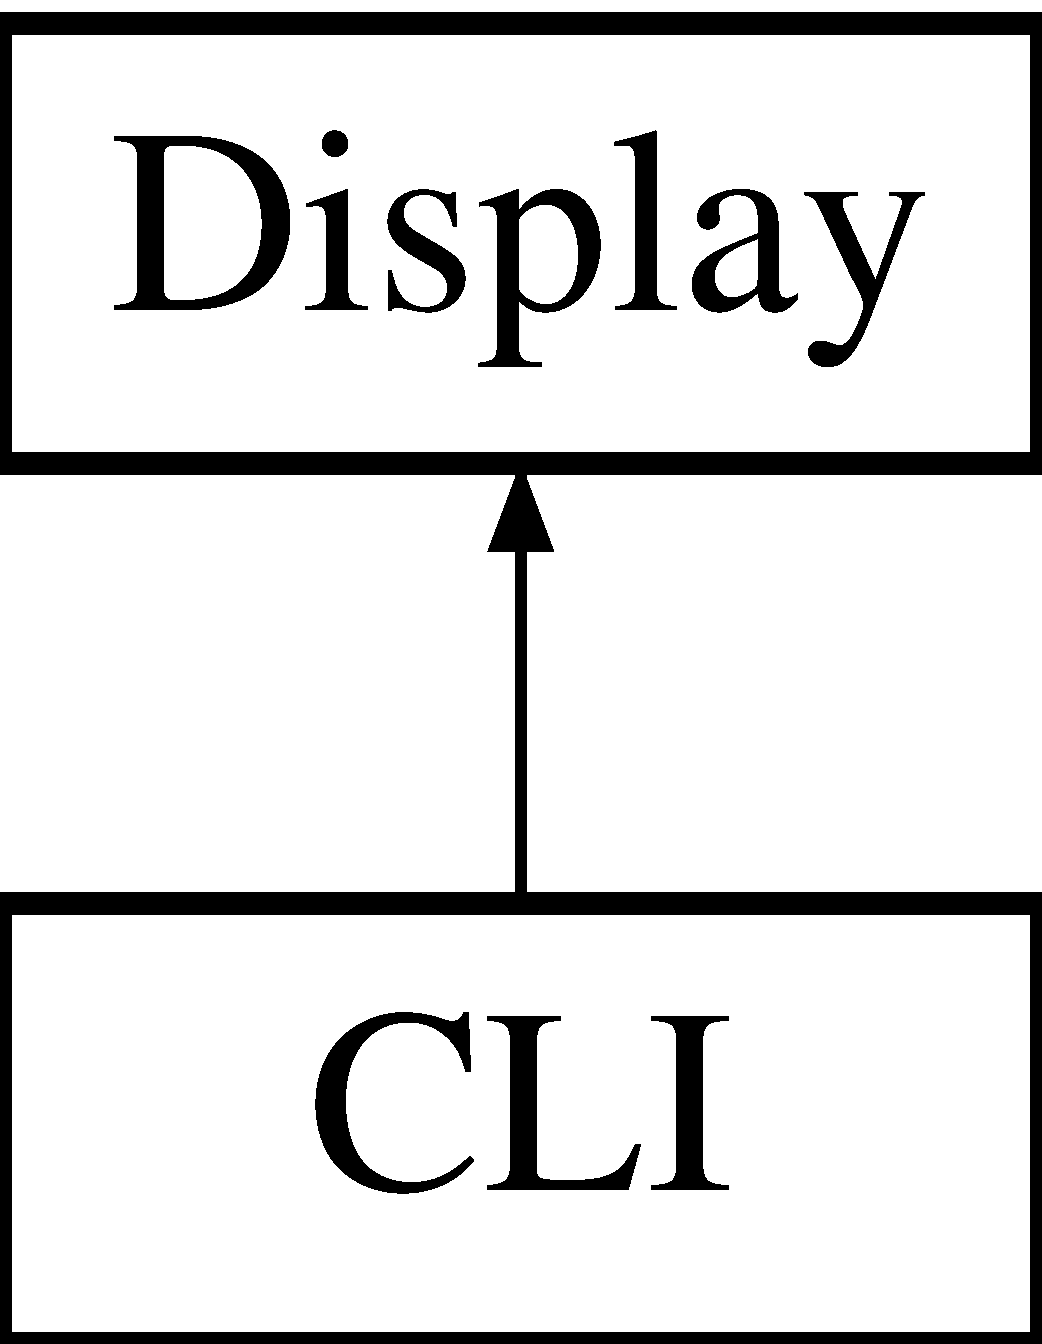
\includegraphics[height=3.000000cm]{classDisplay}
\end{center}
\end{figure}
\subsection*{Fonctions membres publiques}
\begin{DoxyCompactItemize}
\item 
\hyperlink{classDisplay_a46094310ba411f6fea561f799c4d0754}{Display} ()=default
\item 
virtual \hyperlink{classDisplay_a8c364e5ed02f311a695e9502773d1c74}{$\sim$\+Display} ()=default
\item 
virtual void \hyperlink{classDisplay_a55719ab539ee6cc803d9de74b05f8e38}{display\+Login\+Prompt} ()=0
\item 
virtual void \hyperlink{classDisplay_ac4cc71c734feea0099bbeae89e6d2f1c}{display\+Login\+Result} (std\+::string)=0
\item 
virtual void \hyperlink{classDisplay_a93154cf71b945b6ce3ef959a306629f2}{valide\+Login} ()=0
\item 
virtual void \hyperlink{classDisplay_a88a6e0ccafb0ef286149a9ab4ffb28ad}{display\+Main\+Window} ()=0
\end{DoxyCompactItemize}


\subsection{Documentation des constructeurs et destructeur}
\hypertarget{classDisplay_a46094310ba411f6fea561f799c4d0754}{}\index{Display@{Display}!Display@{Display}}
\index{Display@{Display}!Display@{Display}}
\subsubsection[{Display()=default}]{\setlength{\rightskip}{0pt plus 5cm}Display\+::\+Display (
\begin{DoxyParamCaption}
{}
\end{DoxyParamCaption}
)\hspace{0.3cm}{\ttfamily [default]}}\label{classDisplay_a46094310ba411f6fea561f799c4d0754}
\hypertarget{classDisplay_a8c364e5ed02f311a695e9502773d1c74}{}\index{Display@{Display}!````~Display@{$\sim$\+Display}}
\index{````~Display@{$\sim$\+Display}!Display@{Display}}
\subsubsection[{$\sim$\+Display()=default}]{\setlength{\rightskip}{0pt plus 5cm}virtual Display\+::$\sim$\+Display (
\begin{DoxyParamCaption}
{}
\end{DoxyParamCaption}
)\hspace{0.3cm}{\ttfamily [virtual]}, {\ttfamily [default]}}\label{classDisplay_a8c364e5ed02f311a695e9502773d1c74}


\subsection{Documentation des fonctions membres}
\hypertarget{classDisplay_a55719ab539ee6cc803d9de74b05f8e38}{}\index{Display@{Display}!display\+Login\+Prompt@{display\+Login\+Prompt}}
\index{display\+Login\+Prompt@{display\+Login\+Prompt}!Display@{Display}}
\subsubsection[{display\+Login\+Prompt()=0}]{\setlength{\rightskip}{0pt plus 5cm}virtual void Display\+::display\+Login\+Prompt (
\begin{DoxyParamCaption}
{}
\end{DoxyParamCaption}
)\hspace{0.3cm}{\ttfamily [pure virtual]}}\label{classDisplay_a55719ab539ee6cc803d9de74b05f8e38}


Implémenté dans \hyperlink{classCLI_a6cf4acf9f7fa587cc49b892487c68f13}{C\+L\+I}.

\hypertarget{classDisplay_ac4cc71c734feea0099bbeae89e6d2f1c}{}\index{Display@{Display}!display\+Login\+Result@{display\+Login\+Result}}
\index{display\+Login\+Result@{display\+Login\+Result}!Display@{Display}}
\subsubsection[{display\+Login\+Result(std\+::string)=0}]{\setlength{\rightskip}{0pt plus 5cm}virtual void Display\+::display\+Login\+Result (
\begin{DoxyParamCaption}
\item[{std\+::string}]{}
\end{DoxyParamCaption}
)\hspace{0.3cm}{\ttfamily [pure virtual]}}\label{classDisplay_ac4cc71c734feea0099bbeae89e6d2f1c}


Implémenté dans \hyperlink{classCLI_abf864752edc73dba33fce8a0f06137c4}{C\+L\+I}.

\hypertarget{classDisplay_a88a6e0ccafb0ef286149a9ab4ffb28ad}{}\index{Display@{Display}!display\+Main\+Window@{display\+Main\+Window}}
\index{display\+Main\+Window@{display\+Main\+Window}!Display@{Display}}
\subsubsection[{display\+Main\+Window()=0}]{\setlength{\rightskip}{0pt plus 5cm}virtual void Display\+::display\+Main\+Window (
\begin{DoxyParamCaption}
{}
\end{DoxyParamCaption}
)\hspace{0.3cm}{\ttfamily [pure virtual]}}\label{classDisplay_a88a6e0ccafb0ef286149a9ab4ffb28ad}


Implémenté dans \hyperlink{classCLI_abcf6f643c8a94e0451b4b6d9ab9546c7}{C\+L\+I}.

\hypertarget{classDisplay_a93154cf71b945b6ce3ef959a306629f2}{}\index{Display@{Display}!valide\+Login@{valide\+Login}}
\index{valide\+Login@{valide\+Login}!Display@{Display}}
\subsubsection[{valide\+Login()=0}]{\setlength{\rightskip}{0pt plus 5cm}virtual void Display\+::valide\+Login (
\begin{DoxyParamCaption}
{}
\end{DoxyParamCaption}
)\hspace{0.3cm}{\ttfamily [pure virtual]}}\label{classDisplay_a93154cf71b945b6ce3ef959a306629f2}


Implémenté dans \hyperlink{classCLI_ac900759039333051b414c9002dd2100c}{C\+L\+I}.



La documentation de cette classe a été générée à partir du fichier suivant \+:\begin{DoxyCompactItemize}
\item 
client/\hyperlink{Display_8hpp}{Display.\+hpp}\end{DoxyCompactItemize}

\hypertarget{classEffect}{}\section{Référence de la classe Effect}
\label{classEffect}\index{Effect@{Effect}}


{\ttfamily \#include $<$Effect.\+hpp$>$}

\subsection*{Fonctions membres publiques}
\begin{DoxyCompactItemize}
\item 
virtual \hyperlink{classEffect_ae70bfffd7ffd1538c33a2b4590fec0da}{Effect} ()
\item 
virtual \hyperlink{classEffect_ab0f471df484d3ef351b704fef39a7072}{$\sim$\+Effect} ()
\item 
virtual void \hyperlink{classEffect_af75b9e3f53aba579f37cd2a0e30a0296}{apply} (\hyperlink{classCardMonster}{Card\+Monster} $\ast$)=0
\item 
virtual bool \hyperlink{classEffect_adb7655cc87e0602f6f608103ff388a6f}{is\+Taunt} ()
\item 
virtual bool \hyperlink{classEffect_a23e7eba966b28f051ec12865f53cd092}{can\+Be\+Apply\+On\+Player} ()
\item 
virtual bool \hyperlink{classEffect_a81611bfcbbd800ac40b3c38146fb7277}{can\+Be\+Apply\+On\+P\+Card} ()
\end{DoxyCompactItemize}
\subsection*{Fonctions membres publiques statiques}
\begin{DoxyCompactItemize}
\item 
static void \hyperlink{classEffect_ae185e5fd1219ac1d7ffbcd51d0ace58c}{load\+All\+Effect} ()
\item 
static \hyperlink{classEffect}{Effect} $\ast$ \hyperlink{classEffect_a146cdf511868872b7e1879c07c6eb367}{get\+Effect\+By\+I\+D} (std\+::size\+\_\+t)
\end{DoxyCompactItemize}


\subsection{Documentation des constructeurs et destructeur}
\hypertarget{classEffect_ae70bfffd7ffd1538c33a2b4590fec0da}{}\index{Effect@{Effect}!Effect@{Effect}}
\index{Effect@{Effect}!Effect@{Effect}}
\subsubsection[{Effect()}]{\setlength{\rightskip}{0pt plus 5cm}virtual Effect\+::\+Effect (
\begin{DoxyParamCaption}
{}
\end{DoxyParamCaption}
)\hspace{0.3cm}{\ttfamily [inline]}, {\ttfamily [virtual]}}\label{classEffect_ae70bfffd7ffd1538c33a2b4590fec0da}
\hypertarget{classEffect_ab0f471df484d3ef351b704fef39a7072}{}\index{Effect@{Effect}!````~Effect@{$\sim$\+Effect}}
\index{````~Effect@{$\sim$\+Effect}!Effect@{Effect}}
\subsubsection[{$\sim$\+Effect()}]{\setlength{\rightskip}{0pt plus 5cm}virtual Effect\+::$\sim$\+Effect (
\begin{DoxyParamCaption}
{}
\end{DoxyParamCaption}
)\hspace{0.3cm}{\ttfamily [inline]}, {\ttfamily [virtual]}}\label{classEffect_ab0f471df484d3ef351b704fef39a7072}


\subsection{Documentation des fonctions membres}
\hypertarget{classEffect_af75b9e3f53aba579f37cd2a0e30a0296}{}\index{Effect@{Effect}!apply@{apply}}
\index{apply@{apply}!Effect@{Effect}}
\subsubsection[{apply(\+Card\+Monster $\ast$)=0}]{\setlength{\rightskip}{0pt plus 5cm}virtual void Effect\+::apply (
\begin{DoxyParamCaption}
\item[{{\bf Card\+Monster} $\ast$}]{}
\end{DoxyParamCaption}
)\hspace{0.3cm}{\ttfamily [pure virtual]}}\label{classEffect_af75b9e3f53aba579f37cd2a0e30a0296}
\hypertarget{classEffect_a81611bfcbbd800ac40b3c38146fb7277}{}\index{Effect@{Effect}!can\+Be\+Apply\+On\+P\+Card@{can\+Be\+Apply\+On\+P\+Card}}
\index{can\+Be\+Apply\+On\+P\+Card@{can\+Be\+Apply\+On\+P\+Card}!Effect@{Effect}}
\subsubsection[{can\+Be\+Apply\+On\+P\+Card()}]{\setlength{\rightskip}{0pt plus 5cm}virtual bool Effect\+::can\+Be\+Apply\+On\+P\+Card (
\begin{DoxyParamCaption}
{}
\end{DoxyParamCaption}
)\hspace{0.3cm}{\ttfamily [inline]}, {\ttfamily [virtual]}}\label{classEffect_a81611bfcbbd800ac40b3c38146fb7277}
\hypertarget{classEffect_a23e7eba966b28f051ec12865f53cd092}{}\index{Effect@{Effect}!can\+Be\+Apply\+On\+Player@{can\+Be\+Apply\+On\+Player}}
\index{can\+Be\+Apply\+On\+Player@{can\+Be\+Apply\+On\+Player}!Effect@{Effect}}
\subsubsection[{can\+Be\+Apply\+On\+Player()}]{\setlength{\rightskip}{0pt plus 5cm}virtual bool Effect\+::can\+Be\+Apply\+On\+Player (
\begin{DoxyParamCaption}
{}
\end{DoxyParamCaption}
)\hspace{0.3cm}{\ttfamily [inline]}, {\ttfamily [virtual]}}\label{classEffect_a23e7eba966b28f051ec12865f53cd092}
\hypertarget{classEffect_a146cdf511868872b7e1879c07c6eb367}{}\index{Effect@{Effect}!get\+Effect\+By\+I\+D@{get\+Effect\+By\+I\+D}}
\index{get\+Effect\+By\+I\+D@{get\+Effect\+By\+I\+D}!Effect@{Effect}}
\subsubsection[{get\+Effect\+By\+I\+D(std\+::size\+\_\+t)}]{\setlength{\rightskip}{0pt plus 5cm}{\bf Effect} $\ast$ Effect\+::get\+Effect\+By\+I\+D (
\begin{DoxyParamCaption}
\item[{std\+::size\+\_\+t}]{id}
\end{DoxyParamCaption}
)\hspace{0.3cm}{\ttfamily [static]}}\label{classEffect_a146cdf511868872b7e1879c07c6eb367}
\hypertarget{classEffect_adb7655cc87e0602f6f608103ff388a6f}{}\index{Effect@{Effect}!is\+Taunt@{is\+Taunt}}
\index{is\+Taunt@{is\+Taunt}!Effect@{Effect}}
\subsubsection[{is\+Taunt()}]{\setlength{\rightskip}{0pt plus 5cm}virtual bool Effect\+::is\+Taunt (
\begin{DoxyParamCaption}
{}
\end{DoxyParamCaption}
)\hspace{0.3cm}{\ttfamily [inline]}, {\ttfamily [virtual]}}\label{classEffect_adb7655cc87e0602f6f608103ff388a6f}
\hypertarget{classEffect_ae185e5fd1219ac1d7ffbcd51d0ace58c}{}\index{Effect@{Effect}!load\+All\+Effect@{load\+All\+Effect}}
\index{load\+All\+Effect@{load\+All\+Effect}!Effect@{Effect}}
\subsubsection[{load\+All\+Effect()}]{\setlength{\rightskip}{0pt plus 5cm}void Effect\+::load\+All\+Effect (
\begin{DoxyParamCaption}
{}
\end{DoxyParamCaption}
)\hspace{0.3cm}{\ttfamily [static]}}\label{classEffect_ae185e5fd1219ac1d7ffbcd51d0ace58c}


La documentation de cette classe a été générée à partir du fichier suivant \+:\begin{DoxyCompactItemize}
\item 
server/\hyperlink{Effect_8hpp}{Effect.\+hpp}\end{DoxyCompactItemize}

\hypertarget{classFriends}{}\section{Référence de la classe Friends}
\label{classFriends}\index{Friends@{Friends}}


{\ttfamily \#include $<$Friends.\+hpp$>$}

Graphe d\textquotesingle{}héritage de Friends\+:\begin{figure}[H]
\begin{center}
\leavevmode
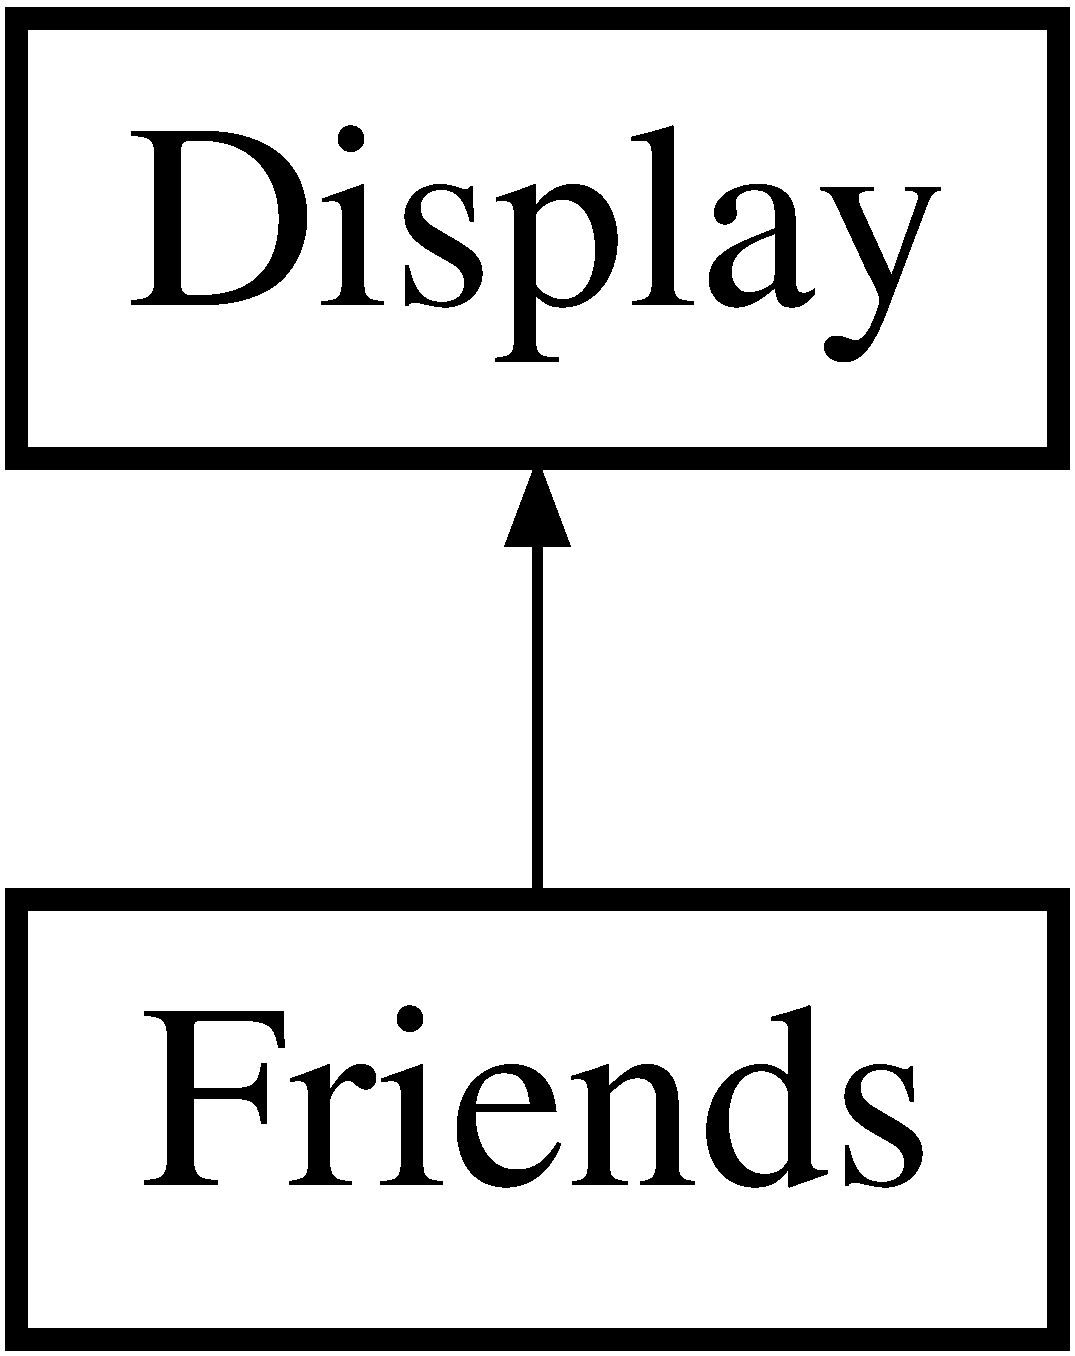
\includegraphics[height=2.000000cm]{classFriends}
\end{center}
\end{figure}
\subsection*{Membres hérités additionnels}


La documentation de cette classe a été générée à partir du fichier suivant \+:\begin{DoxyCompactItemize}
\item 
client/\hyperlink{Friends_8hpp}{Friends.\+hpp}\end{DoxyCompactItemize}

\hypertarget{classFriendsManager}{}\section{Référence de la classe Friends\+Manager}
\label{classFriendsManager}\index{Friends\+Manager@{Friends\+Manager}}


{\ttfamily \#include $<$Friends\+Manager.\+hpp$>$}



\subsection{Description détaillée}
One class per \hyperlink{classPlayer}{Player} 

La documentation de cette classe a été générée à partir du fichier suivant \+:\begin{DoxyCompactItemize}
\item 
server/\hyperlink{FriendsManager_8hpp}{Friends\+Manager.\+hpp}\end{DoxyCompactItemize}

\hypertarget{classGame}{}\section{Référence de la classe Game}
\label{classGame}\index{Game@{Game}}


{\ttfamily \#include $<$Game.\+hpp$>$}

\subsection*{Fonctions membres publiques}
\begin{DoxyCompactItemize}
\item 
\hyperlink{classGame_ad59df6562a58a614fda24622d3715b65}{Game} ()
\item 
\hyperlink{classGame_aa79443880de5f26387c2a1c70c8c1aae}{Game} (const \hyperlink{classGame}{Game} \&)
\item 
\hyperlink{classGame}{Game} \& \hyperlink{classGame_aec1439ca4c76f4a002c235134d590158}{operator=} (const \hyperlink{classGame}{Game} \&)
\item 
virtual \hyperlink{classGame_ab0556d428e8db075b405355af7e81dae}{$\sim$\+Game} ()=default
\item 
void \hyperlink{classGame_a41a8233a0473e2e3687d0380c9b2bccb}{check\+Deck\+And\+Start} ()
\item 
void \hyperlink{classGame_a6d54497ce3a66f6dd45eacfdccc8d0bd}{draw} ()
\item 
void \hyperlink{classGame_a407f859fd79905d6b868de21748123fb}{place\+Card} (\hyperlink{classPlayerInGame}{Player\+In\+Game} $\ast$, \hyperlink{classCard}{Card} $\ast$, \hyperlink{classCardMonster}{Card\+Monster} $\ast$)
\item 
void \hyperlink{classGame_a78b7006c16663d938285c7fd28e6db6b}{place\+Card} (\hyperlink{classPlayerInGame}{Player\+In\+Game} $\ast$, \hyperlink{classCard}{Card} $\ast$, \hyperlink{classPlayerInGame}{Player\+In\+Game} $\ast$)
\item 
void \hyperlink{classGame_ab0de361fcd868ab41245535447f128ec}{attack\+With\+Card} (\hyperlink{classPlayerInGame}{Player\+In\+Game} $\ast$, \hyperlink{classCardMonster}{Card\+Monster} $\ast$, \hyperlink{classCardMonster}{Card\+Monster} $\ast$)
\item 
void \hyperlink{classGame_aea86730a90afb69330ef43d1115a6a4f}{attack\+With\+Card} (\hyperlink{classPlayerInGame}{Player\+In\+Game} $\ast$, \hyperlink{classCardMonster}{Card\+Monster} $\ast$, \hyperlink{classPlayerInGame}{Player\+In\+Game} $\ast$)
\end{DoxyCompactItemize}
\subsection*{Fonctions membres publiques statiques}
\begin{DoxyCompactItemize}
\item 
static void \hyperlink{classGame_ab308d4f03590d8b2b6796f6eaa8a33b3}{add\+Player\+Wait\+Game} (\hyperlink{classPlayer}{Player} player)
\end{DoxyCompactItemize}


\subsection{Description détaillée}
One class per game. Contains the two players and all other information for the game 

\subsection{Documentation des constructeurs et destructeur}
\hypertarget{classGame_ad59df6562a58a614fda24622d3715b65}{}\index{Game@{Game}!Game@{Game}}
\index{Game@{Game}!Game@{Game}}
\subsubsection[{Game()}]{\setlength{\rightskip}{0pt plus 5cm}Game\+::\+Game (
\begin{DoxyParamCaption}
{}
\end{DoxyParamCaption}
)}\label{classGame_ad59df6562a58a614fda24622d3715b65}
Default constructor \hypertarget{classGame_aa79443880de5f26387c2a1c70c8c1aae}{}\index{Game@{Game}!Game@{Game}}
\index{Game@{Game}!Game@{Game}}
\subsubsection[{Game(const Game \&)}]{\setlength{\rightskip}{0pt plus 5cm}Game\+::\+Game (
\begin{DoxyParamCaption}
\item[{const {\bf Game} \&}]{game}
\end{DoxyParamCaption}
)}\label{classGame_aa79443880de5f26387c2a1c70c8c1aae}
\hyperlink{classGame}{Game} constructor


\begin{DoxyParams}{Paramètres}
{\em p1} & the first player \\
\hline
{\em p2} & the second player Copy constructor\\
\hline
{\em game} & who must be copied \\
\hline
\end{DoxyParams}
\hypertarget{classGame_ab0556d428e8db075b405355af7e81dae}{}\index{Game@{Game}!````~Game@{$\sim$\+Game}}
\index{````~Game@{$\sim$\+Game}!Game@{Game}}
\subsubsection[{$\sim$\+Game()=default}]{\setlength{\rightskip}{0pt plus 5cm}virtual Game\+::$\sim$\+Game (
\begin{DoxyParamCaption}
{}
\end{DoxyParamCaption}
)\hspace{0.3cm}{\ttfamily [virtual]}, {\ttfamily [default]}}\label{classGame_ab0556d428e8db075b405355af7e81dae}


\subsection{Documentation des fonctions membres}
\hypertarget{classGame_ab308d4f03590d8b2b6796f6eaa8a33b3}{}\index{Game@{Game}!add\+Player\+Wait\+Game@{add\+Player\+Wait\+Game}}
\index{add\+Player\+Wait\+Game@{add\+Player\+Wait\+Game}!Game@{Game}}
\subsubsection[{add\+Player\+Wait\+Game(\+Player player)}]{\setlength{\rightskip}{0pt plus 5cm}void Game\+::add\+Player\+Wait\+Game (
\begin{DoxyParamCaption}
\item[{{\bf Player}}]{player}
\end{DoxyParamCaption}
)\hspace{0.3cm}{\ttfamily [static]}}\label{classGame_ab308d4f03590d8b2b6796f6eaa8a33b3}
Adds a player to the waiting list If there is more than one player who is waiting, then it creates a \hyperlink{classGame}{Game}


\begin{DoxyParams}{Paramètres}
{\em player} & the new player waiting \\
\hline
\end{DoxyParams}
\hypertarget{classGame_ab0de361fcd868ab41245535447f128ec}{}\index{Game@{Game}!attack\+With\+Card@{attack\+With\+Card}}
\index{attack\+With\+Card@{attack\+With\+Card}!Game@{Game}}
\subsubsection[{attack\+With\+Card(\+Player\+In\+Game $\ast$, Card\+Monster $\ast$, Card\+Monster $\ast$)}]{\setlength{\rightskip}{0pt plus 5cm}void Game\+::attack\+With\+Card (
\begin{DoxyParamCaption}
\item[{{\bf Player\+In\+Game} $\ast$}]{p\+I\+G, }
\item[{{\bf Card\+Monster} $\ast$}]{card, }
\item[{{\bf Card\+Monster} $\ast$}]{target\+Card}
\end{DoxyParamCaption}
)}\label{classGame_ab0de361fcd868ab41245535447f128ec}
Funciton when player attack a card 
\begin{DoxyParams}{Paramètres}
{\em p\+I\+G} & who play \\
\hline
{\em card} & which play \\
\hline
{\em target\+Card} & card which is attack \\
\hline
\end{DoxyParams}
\hypertarget{classGame_aea86730a90afb69330ef43d1115a6a4f}{}\index{Game@{Game}!attack\+With\+Card@{attack\+With\+Card}}
\index{attack\+With\+Card@{attack\+With\+Card}!Game@{Game}}
\subsubsection[{attack\+With\+Card(\+Player\+In\+Game $\ast$, Card\+Monster $\ast$, Player\+In\+Game $\ast$)}]{\setlength{\rightskip}{0pt plus 5cm}void Game\+::attack\+With\+Card (
\begin{DoxyParamCaption}
\item[{{\bf Player\+In\+Game} $\ast$}]{, }
\item[{{\bf Card\+Monster} $\ast$}]{, }
\item[{{\bf Player\+In\+Game} $\ast$}]{}
\end{DoxyParamCaption}
)}\label{classGame_aea86730a90afb69330ef43d1115a6a4f}
\hypertarget{classGame_a41a8233a0473e2e3687d0380c9b2bccb}{}\index{Game@{Game}!check\+Deck\+And\+Start@{check\+Deck\+And\+Start}}
\index{check\+Deck\+And\+Start@{check\+Deck\+And\+Start}!Game@{Game}}
\subsubsection[{check\+Deck\+And\+Start()}]{\setlength{\rightskip}{0pt plus 5cm}void Game\+::check\+Deck\+And\+Start (
\begin{DoxyParamCaption}
{}
\end{DoxyParamCaption}
)}\label{classGame_a41a8233a0473e2e3687d0380c9b2bccb}
Checks if the player have set his deck If all is ok, the game starts \hypertarget{classGame_a6d54497ce3a66f6dd45eacfdccc8d0bd}{}\index{Game@{Game}!draw@{draw}}
\index{draw@{draw}!Game@{Game}}
\subsubsection[{draw()}]{\setlength{\rightskip}{0pt plus 5cm}void Game\+::draw (
\begin{DoxyParamCaption}
{}
\end{DoxyParamCaption}
)}\label{classGame_a6d54497ce3a66f6dd45eacfdccc8d0bd}
\hypertarget{classGame_aec1439ca4c76f4a002c235134d590158}{}\index{Game@{Game}!operator=@{operator=}}
\index{operator=@{operator=}!Game@{Game}}
\subsubsection[{operator=(const Game \&)}]{\setlength{\rightskip}{0pt plus 5cm}{\bf Game} \& Game\+::operator= (
\begin{DoxyParamCaption}
\item[{const {\bf Game} \&}]{game}
\end{DoxyParamCaption}
)}\label{classGame_aec1439ca4c76f4a002c235134d590158}
Copy operator \hypertarget{classGame_a407f859fd79905d6b868de21748123fb}{}\index{Game@{Game}!place\+Card@{place\+Card}}
\index{place\+Card@{place\+Card}!Game@{Game}}
\subsubsection[{place\+Card(\+Player\+In\+Game $\ast$, Card $\ast$, Card\+Monster $\ast$)}]{\setlength{\rightskip}{0pt plus 5cm}void Game\+::place\+Card (
\begin{DoxyParamCaption}
\item[{{\bf Player\+In\+Game} $\ast$}]{p\+I\+G, }
\item[{{\bf Card} $\ast$}]{card\+Placed, }
\item[{{\bf Card\+Monster} $\ast$}]{target\+Card}
\end{DoxyParamCaption}
)}\label{classGame_a407f859fd79905d6b868de21748123fb}
Function when player place card


\begin{DoxyParams}{Paramètres}
{\em p\+I\+G} & player who place the card \\
\hline
{\em card\+Placed} & the card the must be place \\
\hline
{\em target\+Card} & the card which will have the effect if the placed card have it \\
\hline
\end{DoxyParams}
\hypertarget{classGame_a78b7006c16663d938285c7fd28e6db6b}{}\index{Game@{Game}!place\+Card@{place\+Card}}
\index{place\+Card@{place\+Card}!Game@{Game}}
\subsubsection[{place\+Card(\+Player\+In\+Game $\ast$, Card $\ast$, Player\+In\+Game $\ast$)}]{\setlength{\rightskip}{0pt plus 5cm}void Game\+::place\+Card (
\begin{DoxyParamCaption}
\item[{{\bf Player\+In\+Game} $\ast$}]{p\+I\+G, }
\item[{{\bf Card} $\ast$}]{card\+Placed, }
\item[{{\bf Player\+In\+Game} $\ast$}]{target\+Player}
\end{DoxyParamCaption}
)}\label{classGame_a78b7006c16663d938285c7fd28e6db6b}
Function when player place card


\begin{DoxyParams}{Paramètres}
{\em p\+I\+G} & player who place the card \\
\hline
{\em card\+Placed} & the card the must be place \\
\hline
{\em target\+Player} & player who will have the effect if the placed card have it \\
\hline
\end{DoxyParams}


La documentation de cette classe a été générée à partir des fichiers suivants \+:\begin{DoxyCompactItemize}
\item 
server/\hyperlink{Game_8hpp}{Game.\+hpp}\item 
server/\hyperlink{Game_8cpp}{Game.\+cpp}\end{DoxyCompactItemize}

\hypertarget{structPacket_1_1loginRequestPacket}{}\section{Référence de la structure Packet\+:\+:login\+Request\+Packet}
\label{structPacket_1_1loginRequestPacket}\index{Packet\+::login\+Request\+Packet@{Packet\+::login\+Request\+Packet}}


{\ttfamily \#include $<$Packet.\+hpp$>$}

\subsection*{Attributs publics}
\begin{DoxyCompactItemize}
\item 
int \hyperlink{structPacket_1_1loginRequestPacket_a868cc858137d02dfcec0ab588311881c}{I\+D} = \hyperlink{classPacket_ae91c1d355e4c8f0bef5f893747473661aeadd6545e8dfd8e15000a99a5d8346a1}{L\+O\+G\+I\+N\+\_\+\+R\+E\+Q\+\_\+\+I\+D}
\item 
int \hyperlink{structPacket_1_1loginRequestPacket_ae39055594bd945531dae9e02448dc084}{size} = sizeof(char)$\ast$\hyperlink{Packet_8hpp_a5dc814636bf1234a5bb49481556476d1}{M\+A\+X\+\_\+\+P\+S\+E\+U\+D\+O\+\_\+\+S\+I\+Z\+E}$\ast$2
\item 
char \hyperlink{structPacket_1_1loginRequestPacket_aaa36718e5f1c5d8ac6c13e6065502268}{pseudo} \mbox{[}\hyperlink{Packet_8hpp_a5dc814636bf1234a5bb49481556476d1}{M\+A\+X\+\_\+\+P\+S\+E\+U\+D\+O\+\_\+\+S\+I\+Z\+E}\mbox{]}
\item 
char \hyperlink{structPacket_1_1loginRequestPacket_a85c2b868828d558ac942eadfc8c29523}{password} \mbox{[}\hyperlink{Packet_8hpp_a5dc814636bf1234a5bb49481556476d1}{M\+A\+X\+\_\+\+P\+S\+E\+U\+D\+O\+\_\+\+S\+I\+Z\+E}\mbox{]}
\end{DoxyCompactItemize}


\subsection{Documentation des données membres}
\hypertarget{structPacket_1_1loginRequestPacket_a868cc858137d02dfcec0ab588311881c}{}\index{Packet\+::login\+Request\+Packet@{Packet\+::login\+Request\+Packet}!I\+D@{I\+D}}
\index{I\+D@{I\+D}!Packet\+::login\+Request\+Packet@{Packet\+::login\+Request\+Packet}}
\subsubsection[{I\+D}]{\setlength{\rightskip}{0pt plus 5cm}int Packet\+::login\+Request\+Packet\+::\+I\+D = {\bf L\+O\+G\+I\+N\+\_\+\+R\+E\+Q\+\_\+\+I\+D}}\label{structPacket_1_1loginRequestPacket_a868cc858137d02dfcec0ab588311881c}
\hypertarget{structPacket_1_1loginRequestPacket_a85c2b868828d558ac942eadfc8c29523}{}\index{Packet\+::login\+Request\+Packet@{Packet\+::login\+Request\+Packet}!password@{password}}
\index{password@{password}!Packet\+::login\+Request\+Packet@{Packet\+::login\+Request\+Packet}}
\subsubsection[{password}]{\setlength{\rightskip}{0pt plus 5cm}char Packet\+::login\+Request\+Packet\+::password\mbox{[}{\bf M\+A\+X\+\_\+\+P\+S\+E\+U\+D\+O\+\_\+\+S\+I\+Z\+E}\mbox{]}}\label{structPacket_1_1loginRequestPacket_a85c2b868828d558ac942eadfc8c29523}
\hypertarget{structPacket_1_1loginRequestPacket_aaa36718e5f1c5d8ac6c13e6065502268}{}\index{Packet\+::login\+Request\+Packet@{Packet\+::login\+Request\+Packet}!pseudo@{pseudo}}
\index{pseudo@{pseudo}!Packet\+::login\+Request\+Packet@{Packet\+::login\+Request\+Packet}}
\subsubsection[{pseudo}]{\setlength{\rightskip}{0pt plus 5cm}char Packet\+::login\+Request\+Packet\+::pseudo\mbox{[}{\bf M\+A\+X\+\_\+\+P\+S\+E\+U\+D\+O\+\_\+\+S\+I\+Z\+E}\mbox{]}}\label{structPacket_1_1loginRequestPacket_aaa36718e5f1c5d8ac6c13e6065502268}
\hypertarget{structPacket_1_1loginRequestPacket_ae39055594bd945531dae9e02448dc084}{}\index{Packet\+::login\+Request\+Packet@{Packet\+::login\+Request\+Packet}!size@{size}}
\index{size@{size}!Packet\+::login\+Request\+Packet@{Packet\+::login\+Request\+Packet}}
\subsubsection[{size}]{\setlength{\rightskip}{0pt plus 5cm}int Packet\+::login\+Request\+Packet\+::size = sizeof(char)$\ast${\bf M\+A\+X\+\_\+\+P\+S\+E\+U\+D\+O\+\_\+\+S\+I\+Z\+E}$\ast$2}\label{structPacket_1_1loginRequestPacket_ae39055594bd945531dae9e02448dc084}


La documentation de cette structure a été générée à partir du fichier suivant \+:\begin{DoxyCompactItemize}
\item 
common/\hyperlink{Packet_8hpp}{Packet.\+hpp}\end{DoxyCompactItemize}

\hypertarget{structPacket_1_1loginResultPacket}{}\section{Référence de la structure Packet\+:\+:login\+Result\+Packet}
\label{structPacket_1_1loginResultPacket}\index{Packet\+::login\+Result\+Packet@{Packet\+::login\+Result\+Packet}}


{\ttfamily \#include $<$Packet.\+hpp$>$}

\subsection*{Attributs publics}
\begin{DoxyCompactItemize}
\item 
int \hyperlink{structPacket_1_1loginResultPacket_a9fd277c829ba18e929a71a1c0f5fbc60}{I\+D} = \hyperlink{classPacket_ae91c1d355e4c8f0bef5f893747473661adfad7675a2d1418c82df295276cbe695}{L\+O\+G\+I\+N\+\_\+\+R\+E\+S\+\_\+\+I\+D}
\item 
int \hyperlink{structPacket_1_1loginResultPacket_a270afae616b7a7399c2d4c483fcffec6}{size} = sizeof(int)
\item 
int \hyperlink{structPacket_1_1loginResultPacket_a148ad144908a219d1b6adde5c3337a2f}{result\+Code}
\end{DoxyCompactItemize}


\subsection{Documentation des données membres}
\hypertarget{structPacket_1_1loginResultPacket_a9fd277c829ba18e929a71a1c0f5fbc60}{}\index{Packet\+::login\+Result\+Packet@{Packet\+::login\+Result\+Packet}!I\+D@{I\+D}}
\index{I\+D@{I\+D}!Packet\+::login\+Result\+Packet@{Packet\+::login\+Result\+Packet}}
\subsubsection[{I\+D}]{\setlength{\rightskip}{0pt plus 5cm}int Packet\+::login\+Result\+Packet\+::\+I\+D = {\bf L\+O\+G\+I\+N\+\_\+\+R\+E\+S\+\_\+\+I\+D}}\label{structPacket_1_1loginResultPacket_a9fd277c829ba18e929a71a1c0f5fbc60}
\hypertarget{structPacket_1_1loginResultPacket_a148ad144908a219d1b6adde5c3337a2f}{}\index{Packet\+::login\+Result\+Packet@{Packet\+::login\+Result\+Packet}!result\+Code@{result\+Code}}
\index{result\+Code@{result\+Code}!Packet\+::login\+Result\+Packet@{Packet\+::login\+Result\+Packet}}
\subsubsection[{result\+Code}]{\setlength{\rightskip}{0pt plus 5cm}int Packet\+::login\+Result\+Packet\+::result\+Code}\label{structPacket_1_1loginResultPacket_a148ad144908a219d1b6adde5c3337a2f}
\hypertarget{structPacket_1_1loginResultPacket_a270afae616b7a7399c2d4c483fcffec6}{}\index{Packet\+::login\+Result\+Packet@{Packet\+::login\+Result\+Packet}!size@{size}}
\index{size@{size}!Packet\+::login\+Result\+Packet@{Packet\+::login\+Result\+Packet}}
\subsubsection[{size}]{\setlength{\rightskip}{0pt plus 5cm}int Packet\+::login\+Result\+Packet\+::size = sizeof(int)}\label{structPacket_1_1loginResultPacket_a270afae616b7a7399c2d4c483fcffec6}


La documentation de cette structure a été générée à partir du fichier suivant \+:\begin{DoxyCompactItemize}
\item 
common/\hyperlink{Packet_8hpp}{Packet.\+hpp}\end{DoxyCompactItemize}

\hypertarget{structPacket_1_1packet}{}\section{Référence de la structure Packet\+:\+:packet}
\label{structPacket_1_1packet}\index{Packet\+::packet@{Packet\+::packet}}


{\ttfamily \#include $<$Packet.\+hpp$>$}

\subsection*{Attributs publics}
\begin{DoxyCompactItemize}
\item 
int \hyperlink{structPacket_1_1packet_a6a964ed4653dedd272f901fa77fc98b0}{I\+D}
\item 
int \hyperlink{structPacket_1_1packet_a4acd14895382f87f51cb4c0465de0397}{size} = 0
\end{DoxyCompactItemize}


\subsection{Documentation des données membres}
\hypertarget{structPacket_1_1packet_a6a964ed4653dedd272f901fa77fc98b0}{}\index{Packet\+::packet@{Packet\+::packet}!I\+D@{I\+D}}
\index{I\+D@{I\+D}!Packet\+::packet@{Packet\+::packet}}
\subsubsection[{I\+D}]{\setlength{\rightskip}{0pt plus 5cm}int Packet\+::packet\+::\+I\+D}\label{structPacket_1_1packet_a6a964ed4653dedd272f901fa77fc98b0}
\hypertarget{structPacket_1_1packet_a4acd14895382f87f51cb4c0465de0397}{}\index{Packet\+::packet@{Packet\+::packet}!size@{size}}
\index{size@{size}!Packet\+::packet@{Packet\+::packet}}
\subsubsection[{size}]{\setlength{\rightskip}{0pt plus 5cm}int Packet\+::packet\+::size = 0}\label{structPacket_1_1packet_a4acd14895382f87f51cb4c0465de0397}


La documentation de cette structure a été générée à partir du fichier suivant \+:\begin{DoxyCompactItemize}
\item 
common/\hyperlink{Packet_8hpp}{Packet.\+hpp}\end{DoxyCompactItemize}

\hypertarget{classPacket}{}\section{Référence de la classe Packet}
\label{classPacket}\index{Packet@{Packet}}


{\ttfamily \#include $<$Packet.\+hpp$>$}

\subsection*{Classes}
\begin{DoxyCompactItemize}
\item 
struct \hyperlink{structPacket_1_1carteInfosPacket}{carte\+Infos\+Packet}
\item 
struct \hyperlink{structPacket_1_1carteRequestPacket}{carte\+Request\+Packet}
\item 
struct \hyperlink{structPacket_1_1collectionListPacket}{collection\+List\+Packet}
\item 
struct \hyperlink{structPacket_1_1deckContentPacket}{deck\+Content\+Packet}
\item 
struct \hyperlink{structPacket_1_1deckRequestPacket}{deck\+Request\+Packet}
\item 
struct \hyperlink{structPacket_1_1loginRequestPacket}{login\+Request\+Packet}
\item 
struct \hyperlink{structPacket_1_1loginResultPacket}{login\+Result\+Packet}
\item 
struct \hyperlink{structPacket_1_1packet}{packet}
\end{DoxyCompactItemize}
\subsection*{Types publics}
\begin{DoxyCompactItemize}
\item 
enum \hyperlink{classPacket_ae91c1d355e4c8f0bef5f893747473661}{I\+D\+List} \{ \\*
\hyperlink{classPacket_ae91c1d355e4c8f0bef5f893747473661aeadd6545e8dfd8e15000a99a5d8346a1}{L\+O\+G\+I\+N\+\_\+\+R\+E\+Q\+\_\+\+I\+D} = 11, 
\hyperlink{classPacket_ae91c1d355e4c8f0bef5f893747473661aa44e680c41bfd846ab0225c50660a459}{R\+E\+G\+I\+S\+T\+\_\+\+R\+E\+Q\+\_\+\+I\+D} = 12, 
\hyperlink{classPacket_ae91c1d355e4c8f0bef5f893747473661adfad7675a2d1418c82df295276cbe695}{L\+O\+G\+I\+N\+\_\+\+R\+E\+S\+\_\+\+I\+D} = 13, 
\hyperlink{classPacket_ae91c1d355e4c8f0bef5f893747473661ae4ec5a8eaa644872b70450eeb6e66ec2}{D\+I\+S\+C\+O\+N\+N\+E\+C\+T\+\_\+\+I\+D} = 14, 
\\*
\hyperlink{classPacket_ae91c1d355e4c8f0bef5f893747473661ad94d178cd47baea6d1345dfb581182f3}{C\+O\+L\+L\+E\+C\+T\+I\+O\+N\+\_\+\+R\+E\+Q\+\_\+\+I\+D} = 21, 
\hyperlink{classPacket_ae91c1d355e4c8f0bef5f893747473661a257c56805034a2a1288c8b627f7c4e42}{C\+O\+L\+L\+E\+C\+T\+I\+O\+N\+\_\+\+L\+I\+S\+T\+\_\+\+I\+D} = 22, 
\hyperlink{classPacket_ae91c1d355e4c8f0bef5f893747473661aa0822f1f646c2ea8411b06af9f6fc40c}{D\+E\+C\+K\+\_\+\+R\+E\+Q\+\_\+\+I\+D} = 23, 
\hyperlink{classPacket_ae91c1d355e4c8f0bef5f893747473661ac6762b082af175037f3df2c4079553df}{D\+E\+C\+K\+\_\+\+C\+O\+N\+T\+\_\+\+I\+D} = 24, 
\\*
\hyperlink{classPacket_ae91c1d355e4c8f0bef5f893747473661a1afad4125bf1222a1b4f3201cb29ab3b}{C\+A\+R\+T\+E\+\_\+\+R\+E\+Q\+\_\+\+I\+D} = 25, 
\hyperlink{classPacket_ae91c1d355e4c8f0bef5f893747473661aa61d9c1d39512a3a4054cbfc15a60b48}{C\+A\+R\+T\+E\+\_\+\+I\+N\+F\+O\+\_\+\+I\+D} = 26, 
\hyperlink{classPacket_ae91c1d355e4c8f0bef5f893747473661aea1cc863253ebe274fefcedada1bb62b}{T\+C\+H\+A\+T\+\_\+\+C\+O\+N\+V\+\_\+\+R\+E\+Q\+\_\+\+I\+D} = 31, 
\hyperlink{classPacket_ae91c1d355e4c8f0bef5f893747473661ab503c0a36e7fd992a13db8a4934586ef}{T\+C\+H\+A\+T\+\_\+\+N\+E\+W\+\_\+\+C\+O\+N\+V\+\_\+\+I\+D} = 32, 
\\*
\hyperlink{classPacket_ae91c1d355e4c8f0bef5f893747473661adb5bc9e3b5eb4003e95130132c1162a0}{T\+C\+H\+A\+T\+\_\+\+M\+E\+S\+S\+A\+G\+E\+\_\+\+I\+D} = 33, 
\hyperlink{classPacket_ae91c1d355e4c8f0bef5f893747473661a81b67eb89eaf62145743464b6df6ad5c}{T\+C\+H\+A\+T\+\_\+\+E\+N\+D\+\_\+\+R\+E\+Q\+\_\+\+I\+D} = 34, 
\hyperlink{classPacket_ae91c1d355e4c8f0bef5f893747473661ac0e468e4743cc6b8642f5207ef4cb59a}{T\+C\+H\+A\+T\+\_\+\+E\+N\+D\+\_\+\+C\+O\+N\+V\+\_\+\+I\+D} = 35
 \}
\end{DoxyCompactItemize}
\subsection*{Attributs publics statiques}
\begin{DoxyCompactItemize}
\item 
static const int \hyperlink{classPacket_a4d3ec46364b14d6f59e550920ec9a78a}{packet\+Size} = sizeof(int)$\ast$2
\item 
static const int \hyperlink{classPacket_ab2ef9ab81c25a39ca3a09b954a5765a2}{packet\+Max\+Size} = sizeof(int\mbox{[}200\mbox{]})+\hyperlink{classPacket_a4d3ec46364b14d6f59e550920ec9a78a}{packet\+Size}
\end{DoxyCompactItemize}


\subsection{Documentation des énumérations membres}
\hypertarget{classPacket_ae91c1d355e4c8f0bef5f893747473661}{}\index{Packet@{Packet}!I\+D\+List@{I\+D\+List}}
\index{I\+D\+List@{I\+D\+List}!Packet@{Packet}}
\subsubsection[{I\+D\+List}]{\setlength{\rightskip}{0pt plus 5cm}enum {\bf Packet\+::\+I\+D\+List}}\label{classPacket_ae91c1d355e4c8f0bef5f893747473661}
\begin{Desc}
\item[Valeurs énumérées]\par
\begin{description}
\index{L\+O\+G\+I\+N\+\_\+\+R\+E\+Q\+\_\+\+I\+D@{L\+O\+G\+I\+N\+\_\+\+R\+E\+Q\+\_\+\+I\+D}!Packet@{Packet}}\index{Packet@{Packet}!L\+O\+G\+I\+N\+\_\+\+R\+E\+Q\+\_\+\+I\+D@{L\+O\+G\+I\+N\+\_\+\+R\+E\+Q\+\_\+\+I\+D}}\item[{\em 
\hypertarget{classPacket_ae91c1d355e4c8f0bef5f893747473661aeadd6545e8dfd8e15000a99a5d8346a1}{}L\+O\+G\+I\+N\+\_\+\+R\+E\+Q\+\_\+\+I\+D\label{classPacket_ae91c1d355e4c8f0bef5f893747473661aeadd6545e8dfd8e15000a99a5d8346a1}
}]\index{R\+E\+G\+I\+S\+T\+\_\+\+R\+E\+Q\+\_\+\+I\+D@{R\+E\+G\+I\+S\+T\+\_\+\+R\+E\+Q\+\_\+\+I\+D}!Packet@{Packet}}\index{Packet@{Packet}!R\+E\+G\+I\+S\+T\+\_\+\+R\+E\+Q\+\_\+\+I\+D@{R\+E\+G\+I\+S\+T\+\_\+\+R\+E\+Q\+\_\+\+I\+D}}\item[{\em 
\hypertarget{classPacket_ae91c1d355e4c8f0bef5f893747473661aa44e680c41bfd846ab0225c50660a459}{}R\+E\+G\+I\+S\+T\+\_\+\+R\+E\+Q\+\_\+\+I\+D\label{classPacket_ae91c1d355e4c8f0bef5f893747473661aa44e680c41bfd846ab0225c50660a459}
}]\index{L\+O\+G\+I\+N\+\_\+\+R\+E\+S\+\_\+\+I\+D@{L\+O\+G\+I\+N\+\_\+\+R\+E\+S\+\_\+\+I\+D}!Packet@{Packet}}\index{Packet@{Packet}!L\+O\+G\+I\+N\+\_\+\+R\+E\+S\+\_\+\+I\+D@{L\+O\+G\+I\+N\+\_\+\+R\+E\+S\+\_\+\+I\+D}}\item[{\em 
\hypertarget{classPacket_ae91c1d355e4c8f0bef5f893747473661adfad7675a2d1418c82df295276cbe695}{}L\+O\+G\+I\+N\+\_\+\+R\+E\+S\+\_\+\+I\+D\label{classPacket_ae91c1d355e4c8f0bef5f893747473661adfad7675a2d1418c82df295276cbe695}
}]\index{D\+I\+S\+C\+O\+N\+N\+E\+C\+T\+\_\+\+I\+D@{D\+I\+S\+C\+O\+N\+N\+E\+C\+T\+\_\+\+I\+D}!Packet@{Packet}}\index{Packet@{Packet}!D\+I\+S\+C\+O\+N\+N\+E\+C\+T\+\_\+\+I\+D@{D\+I\+S\+C\+O\+N\+N\+E\+C\+T\+\_\+\+I\+D}}\item[{\em 
\hypertarget{classPacket_ae91c1d355e4c8f0bef5f893747473661ae4ec5a8eaa644872b70450eeb6e66ec2}{}D\+I\+S\+C\+O\+N\+N\+E\+C\+T\+\_\+\+I\+D\label{classPacket_ae91c1d355e4c8f0bef5f893747473661ae4ec5a8eaa644872b70450eeb6e66ec2}
}]\index{C\+O\+L\+L\+E\+C\+T\+I\+O\+N\+\_\+\+R\+E\+Q\+\_\+\+I\+D@{C\+O\+L\+L\+E\+C\+T\+I\+O\+N\+\_\+\+R\+E\+Q\+\_\+\+I\+D}!Packet@{Packet}}\index{Packet@{Packet}!C\+O\+L\+L\+E\+C\+T\+I\+O\+N\+\_\+\+R\+E\+Q\+\_\+\+I\+D@{C\+O\+L\+L\+E\+C\+T\+I\+O\+N\+\_\+\+R\+E\+Q\+\_\+\+I\+D}}\item[{\em 
\hypertarget{classPacket_ae91c1d355e4c8f0bef5f893747473661ad94d178cd47baea6d1345dfb581182f3}{}C\+O\+L\+L\+E\+C\+T\+I\+O\+N\+\_\+\+R\+E\+Q\+\_\+\+I\+D\label{classPacket_ae91c1d355e4c8f0bef5f893747473661ad94d178cd47baea6d1345dfb581182f3}
}]\index{C\+O\+L\+L\+E\+C\+T\+I\+O\+N\+\_\+\+L\+I\+S\+T\+\_\+\+I\+D@{C\+O\+L\+L\+E\+C\+T\+I\+O\+N\+\_\+\+L\+I\+S\+T\+\_\+\+I\+D}!Packet@{Packet}}\index{Packet@{Packet}!C\+O\+L\+L\+E\+C\+T\+I\+O\+N\+\_\+\+L\+I\+S\+T\+\_\+\+I\+D@{C\+O\+L\+L\+E\+C\+T\+I\+O\+N\+\_\+\+L\+I\+S\+T\+\_\+\+I\+D}}\item[{\em 
\hypertarget{classPacket_ae91c1d355e4c8f0bef5f893747473661a257c56805034a2a1288c8b627f7c4e42}{}C\+O\+L\+L\+E\+C\+T\+I\+O\+N\+\_\+\+L\+I\+S\+T\+\_\+\+I\+D\label{classPacket_ae91c1d355e4c8f0bef5f893747473661a257c56805034a2a1288c8b627f7c4e42}
}]\index{D\+E\+C\+K\+\_\+\+R\+E\+Q\+\_\+\+I\+D@{D\+E\+C\+K\+\_\+\+R\+E\+Q\+\_\+\+I\+D}!Packet@{Packet}}\index{Packet@{Packet}!D\+E\+C\+K\+\_\+\+R\+E\+Q\+\_\+\+I\+D@{D\+E\+C\+K\+\_\+\+R\+E\+Q\+\_\+\+I\+D}}\item[{\em 
\hypertarget{classPacket_ae91c1d355e4c8f0bef5f893747473661aa0822f1f646c2ea8411b06af9f6fc40c}{}D\+E\+C\+K\+\_\+\+R\+E\+Q\+\_\+\+I\+D\label{classPacket_ae91c1d355e4c8f0bef5f893747473661aa0822f1f646c2ea8411b06af9f6fc40c}
}]\index{D\+E\+C\+K\+\_\+\+C\+O\+N\+T\+\_\+\+I\+D@{D\+E\+C\+K\+\_\+\+C\+O\+N\+T\+\_\+\+I\+D}!Packet@{Packet}}\index{Packet@{Packet}!D\+E\+C\+K\+\_\+\+C\+O\+N\+T\+\_\+\+I\+D@{D\+E\+C\+K\+\_\+\+C\+O\+N\+T\+\_\+\+I\+D}}\item[{\em 
\hypertarget{classPacket_ae91c1d355e4c8f0bef5f893747473661ac6762b082af175037f3df2c4079553df}{}D\+E\+C\+K\+\_\+\+C\+O\+N\+T\+\_\+\+I\+D\label{classPacket_ae91c1d355e4c8f0bef5f893747473661ac6762b082af175037f3df2c4079553df}
}]\index{C\+A\+R\+T\+E\+\_\+\+R\+E\+Q\+\_\+\+I\+D@{C\+A\+R\+T\+E\+\_\+\+R\+E\+Q\+\_\+\+I\+D}!Packet@{Packet}}\index{Packet@{Packet}!C\+A\+R\+T\+E\+\_\+\+R\+E\+Q\+\_\+\+I\+D@{C\+A\+R\+T\+E\+\_\+\+R\+E\+Q\+\_\+\+I\+D}}\item[{\em 
\hypertarget{classPacket_ae91c1d355e4c8f0bef5f893747473661a1afad4125bf1222a1b4f3201cb29ab3b}{}C\+A\+R\+T\+E\+\_\+\+R\+E\+Q\+\_\+\+I\+D\label{classPacket_ae91c1d355e4c8f0bef5f893747473661a1afad4125bf1222a1b4f3201cb29ab3b}
}]\index{C\+A\+R\+T\+E\+\_\+\+I\+N\+F\+O\+\_\+\+I\+D@{C\+A\+R\+T\+E\+\_\+\+I\+N\+F\+O\+\_\+\+I\+D}!Packet@{Packet}}\index{Packet@{Packet}!C\+A\+R\+T\+E\+\_\+\+I\+N\+F\+O\+\_\+\+I\+D@{C\+A\+R\+T\+E\+\_\+\+I\+N\+F\+O\+\_\+\+I\+D}}\item[{\em 
\hypertarget{classPacket_ae91c1d355e4c8f0bef5f893747473661aa61d9c1d39512a3a4054cbfc15a60b48}{}C\+A\+R\+T\+E\+\_\+\+I\+N\+F\+O\+\_\+\+I\+D\label{classPacket_ae91c1d355e4c8f0bef5f893747473661aa61d9c1d39512a3a4054cbfc15a60b48}
}]\index{T\+C\+H\+A\+T\+\_\+\+C\+O\+N\+V\+\_\+\+R\+E\+Q\+\_\+\+I\+D@{T\+C\+H\+A\+T\+\_\+\+C\+O\+N\+V\+\_\+\+R\+E\+Q\+\_\+\+I\+D}!Packet@{Packet}}\index{Packet@{Packet}!T\+C\+H\+A\+T\+\_\+\+C\+O\+N\+V\+\_\+\+R\+E\+Q\+\_\+\+I\+D@{T\+C\+H\+A\+T\+\_\+\+C\+O\+N\+V\+\_\+\+R\+E\+Q\+\_\+\+I\+D}}\item[{\em 
\hypertarget{classPacket_ae91c1d355e4c8f0bef5f893747473661aea1cc863253ebe274fefcedada1bb62b}{}T\+C\+H\+A\+T\+\_\+\+C\+O\+N\+V\+\_\+\+R\+E\+Q\+\_\+\+I\+D\label{classPacket_ae91c1d355e4c8f0bef5f893747473661aea1cc863253ebe274fefcedada1bb62b}
}]\index{T\+C\+H\+A\+T\+\_\+\+N\+E\+W\+\_\+\+C\+O\+N\+V\+\_\+\+I\+D@{T\+C\+H\+A\+T\+\_\+\+N\+E\+W\+\_\+\+C\+O\+N\+V\+\_\+\+I\+D}!Packet@{Packet}}\index{Packet@{Packet}!T\+C\+H\+A\+T\+\_\+\+N\+E\+W\+\_\+\+C\+O\+N\+V\+\_\+\+I\+D@{T\+C\+H\+A\+T\+\_\+\+N\+E\+W\+\_\+\+C\+O\+N\+V\+\_\+\+I\+D}}\item[{\em 
\hypertarget{classPacket_ae91c1d355e4c8f0bef5f893747473661ab503c0a36e7fd992a13db8a4934586ef}{}T\+C\+H\+A\+T\+\_\+\+N\+E\+W\+\_\+\+C\+O\+N\+V\+\_\+\+I\+D\label{classPacket_ae91c1d355e4c8f0bef5f893747473661ab503c0a36e7fd992a13db8a4934586ef}
}]\index{T\+C\+H\+A\+T\+\_\+\+M\+E\+S\+S\+A\+G\+E\+\_\+\+I\+D@{T\+C\+H\+A\+T\+\_\+\+M\+E\+S\+S\+A\+G\+E\+\_\+\+I\+D}!Packet@{Packet}}\index{Packet@{Packet}!T\+C\+H\+A\+T\+\_\+\+M\+E\+S\+S\+A\+G\+E\+\_\+\+I\+D@{T\+C\+H\+A\+T\+\_\+\+M\+E\+S\+S\+A\+G\+E\+\_\+\+I\+D}}\item[{\em 
\hypertarget{classPacket_ae91c1d355e4c8f0bef5f893747473661adb5bc9e3b5eb4003e95130132c1162a0}{}T\+C\+H\+A\+T\+\_\+\+M\+E\+S\+S\+A\+G\+E\+\_\+\+I\+D\label{classPacket_ae91c1d355e4c8f0bef5f893747473661adb5bc9e3b5eb4003e95130132c1162a0}
}]\index{T\+C\+H\+A\+T\+\_\+\+E\+N\+D\+\_\+\+R\+E\+Q\+\_\+\+I\+D@{T\+C\+H\+A\+T\+\_\+\+E\+N\+D\+\_\+\+R\+E\+Q\+\_\+\+I\+D}!Packet@{Packet}}\index{Packet@{Packet}!T\+C\+H\+A\+T\+\_\+\+E\+N\+D\+\_\+\+R\+E\+Q\+\_\+\+I\+D@{T\+C\+H\+A\+T\+\_\+\+E\+N\+D\+\_\+\+R\+E\+Q\+\_\+\+I\+D}}\item[{\em 
\hypertarget{classPacket_ae91c1d355e4c8f0bef5f893747473661a81b67eb89eaf62145743464b6df6ad5c}{}T\+C\+H\+A\+T\+\_\+\+E\+N\+D\+\_\+\+R\+E\+Q\+\_\+\+I\+D\label{classPacket_ae91c1d355e4c8f0bef5f893747473661a81b67eb89eaf62145743464b6df6ad5c}
}]\index{T\+C\+H\+A\+T\+\_\+\+E\+N\+D\+\_\+\+C\+O\+N\+V\+\_\+\+I\+D@{T\+C\+H\+A\+T\+\_\+\+E\+N\+D\+\_\+\+C\+O\+N\+V\+\_\+\+I\+D}!Packet@{Packet}}\index{Packet@{Packet}!T\+C\+H\+A\+T\+\_\+\+E\+N\+D\+\_\+\+C\+O\+N\+V\+\_\+\+I\+D@{T\+C\+H\+A\+T\+\_\+\+E\+N\+D\+\_\+\+C\+O\+N\+V\+\_\+\+I\+D}}\item[{\em 
\hypertarget{classPacket_ae91c1d355e4c8f0bef5f893747473661ac0e468e4743cc6b8642f5207ef4cb59a}{}T\+C\+H\+A\+T\+\_\+\+E\+N\+D\+\_\+\+C\+O\+N\+V\+\_\+\+I\+D\label{classPacket_ae91c1d355e4c8f0bef5f893747473661ac0e468e4743cc6b8642f5207ef4cb59a}
}]\end{description}
\end{Desc}


\subsection{Documentation des données membres}
\hypertarget{classPacket_ab2ef9ab81c25a39ca3a09b954a5765a2}{}\index{Packet@{Packet}!packet\+Max\+Size@{packet\+Max\+Size}}
\index{packet\+Max\+Size@{packet\+Max\+Size}!Packet@{Packet}}
\subsubsection[{packet\+Max\+Size}]{\setlength{\rightskip}{0pt plus 5cm}const int Packet\+::packet\+Max\+Size = sizeof(int\mbox{[}200\mbox{]})+{\bf packet\+Size}\hspace{0.3cm}{\ttfamily [static]}}\label{classPacket_ab2ef9ab81c25a39ca3a09b954a5765a2}
\hypertarget{classPacket_a4d3ec46364b14d6f59e550920ec9a78a}{}\index{Packet@{Packet}!packet\+Size@{packet\+Size}}
\index{packet\+Size@{packet\+Size}!Packet@{Packet}}
\subsubsection[{packet\+Size}]{\setlength{\rightskip}{0pt plus 5cm}const int Packet\+::packet\+Size = sizeof(int)$\ast$2\hspace{0.3cm}{\ttfamily [static]}}\label{classPacket_a4d3ec46364b14d6f59e550920ec9a78a}


La documentation de cette classe a été générée à partir du fichier suivant \+:\begin{DoxyCompactItemize}
\item 
common/\hyperlink{Packet_8hpp}{Packet.\+hpp}\end{DoxyCompactItemize}

\hypertarget{classPlayer}{}\section{Référence de la classe Player}
\label{classPlayer}\index{Player@{Player}}


{\ttfamily \#include $<$Player.\+hpp$>$}

Graphe d\textquotesingle{}héritage de Player\+:\begin{figure}[H]
\begin{center}
\leavevmode
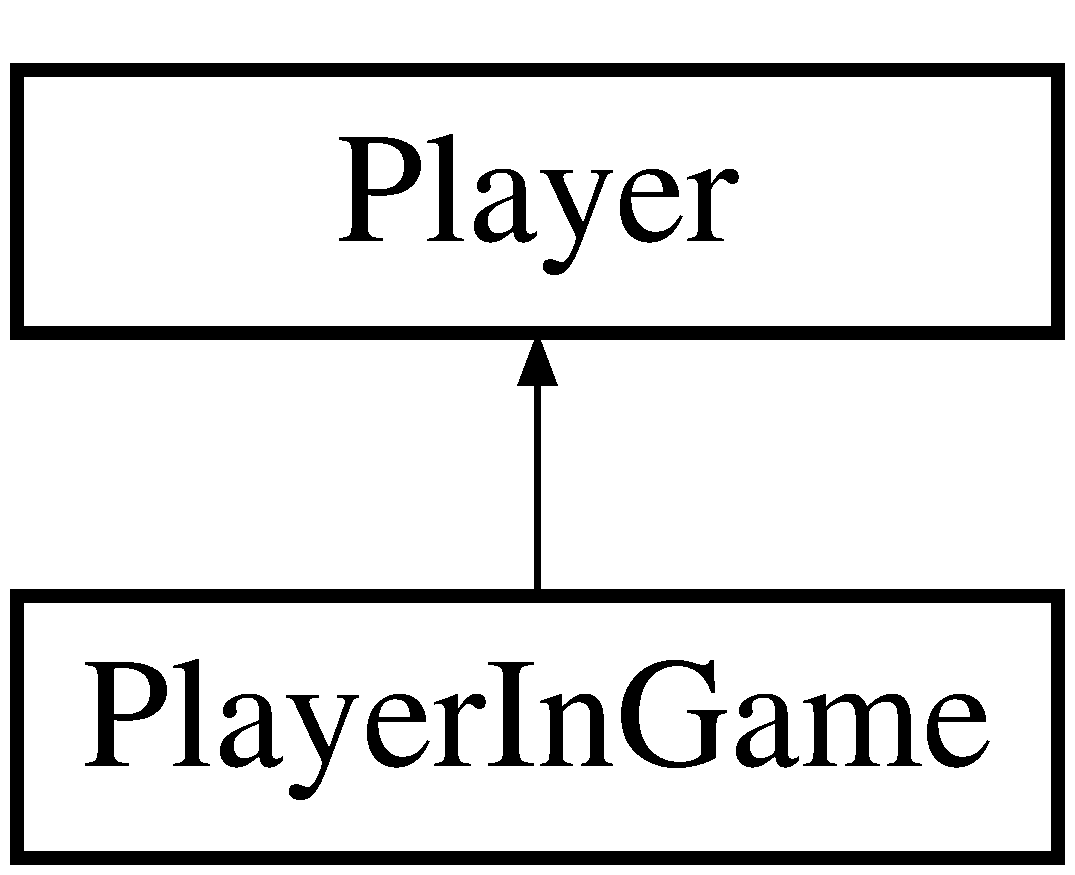
\includegraphics[height=2.000000cm]{classPlayer}
\end{center}
\end{figure}
\subsection*{Fonctions membres publiques}
\begin{DoxyCompactItemize}
\item 
\hyperlink{classPlayer_aaa23b3bf80e8c0267cf08d4fe4d6ddc1}{Player} ()=default
\item 
\hyperlink{classPlayer_a9e88d178553a82a6c7406b8ff78e1beb}{Player} (\hyperlink{CardManager_8hpp_ab701e3ac61a85b337ec5c1abaad6742d}{nlohmann\+::json} \&, int sockfd=0)
\item 
void \hyperlink{classPlayer_a224828ffebbc85cda6a370eb7fab7332}{adjudicate\+Victory} ()
\item 
\hyperlink{Error_8hpp_a2c3e4bb40f36b262a5214e2da2bca9c5}{Error} \hyperlink{classPlayer_ad6b7d88cbcd56aeb046c154fdedeb52e}{add\+Card\+Collection} (\hyperlink{classCard}{Card} $\ast$c)
\item 
void \hyperlink{classPlayer_a882d9db35e3277bcd2db52fa9eca7dfb}{adjudicate\+Defeat} ()
\item 
void \hyperlink{classPlayer_adf7cea3607c835e1c32f054524cd3027}{update\+Sockfd} (int a)
\item 
std\+::string \hyperlink{classPlayer_ad4c6a95f1cf69c44d0c585465b101c70}{get\+Name} () const 
\item 
std\+::string \hyperlink{classPlayer_a244625f85468369c2dd4115d10dd96c0}{get\+Pass} () const 
\item 
unsigned \hyperlink{classPlayer_a6cce4ff00f12069ee17a0c8d8be7912a}{get\+Victories} () const 
\item 
unsigned \hyperlink{classPlayer_ac8d227b243a10660a092e289365d4f13}{get\+Defeats} () const 
\item 
\hyperlink{classDeck}{Deck} $\ast$ \hyperlink{classPlayer_a24e81b3a057a93babe3ff469d59cecd3}{get\+Deck} (std\+::string deck\+Name)
\item 
bool \hyperlink{classPlayer_af7f21437111ed192905e76777e1cfcff}{remove\+Deck} (\hyperlink{classDeck}{Deck} $\ast$)
\item 
std\+::string \hyperlink{classPlayer_a03a285ddda49ed0c0383b39a0a5f415b}{serialise} () const 
\item 
bool \hyperlink{classPlayer_ad595a59902a36610d2aa8d496a071f1f}{operator==} (const std\+::string \&) const 
\item 
bool \hyperlink{classPlayer_ab8344f240fbc64e17012fea952bf5821}{operator$<$} (const \hyperlink{classPlayer}{Player} \&) const 
\item 
virtual \hyperlink{classPlayer_a11017c0ed8a639f3b1308ab167fbeca2}{$\sim$\+Player} ()=default
\end{DoxyCompactItemize}
\subsection*{Fonctions membres protégées}
\begin{DoxyCompactItemize}
\item 
std\+::vector$<$ \hyperlink{classDeck}{Deck} $\ast$ $>$ \hyperlink{classPlayer_ad3e0232a0013556f3dc6a7cf3219c5e3}{get\+List\+Deck} ()
\end{DoxyCompactItemize}
\subsection*{Attributs protégés}
\begin{DoxyCompactItemize}
\item 
unsigned \hyperlink{classPlayer_aa9529e5da5724425ef1e94fb3f5b791f}{\+\_\+victories}
\item 
unsigned \hyperlink{classPlayer_aa3e1c71c5439841e5f3728c2a567344e}{\+\_\+defeats}
\end{DoxyCompactItemize}
\subsection*{Amis}
\begin{DoxyCompactItemize}
\item 
std\+::ostream \& \hyperlink{classPlayer_a09ccce2cf3a3aaa6af4721b94eb301d9}{operator$<$$<$} (std\+::ostream \&, const \hyperlink{classPlayer}{Player} \&)
\item 
std\+::string \& \hyperlink{classPlayer_ae196d81b10472c3768f788280aaf392b}{operator$<$$<$} (std\+::string \&, const \hyperlink{classPlayer}{Player} \&)
\end{DoxyCompactItemize}


\subsection{Description détaillée}
One class per player. This object stocks the socket to communicate with player When the server starts, he must load all Players 

\subsection{Documentation des constructeurs et destructeur}
\hypertarget{classPlayer_aaa23b3bf80e8c0267cf08d4fe4d6ddc1}{}\index{Player@{Player}!Player@{Player}}
\index{Player@{Player}!Player@{Player}}
\subsubsection[{Player()=default}]{\setlength{\rightskip}{0pt plus 5cm}Player\+::\+Player (
\begin{DoxyParamCaption}
{}
\end{DoxyParamCaption}
)\hspace{0.3cm}{\ttfamily [default]}}\label{classPlayer_aaa23b3bf80e8c0267cf08d4fe4d6ddc1}
\hypertarget{classPlayer_a9e88d178553a82a6c7406b8ff78e1beb}{}\index{Player@{Player}!Player@{Player}}
\index{Player@{Player}!Player@{Player}}
\subsubsection[{Player(nlohmann\+::json \&, int sockfd=0)}]{\setlength{\rightskip}{0pt plus 5cm}Player\+::\+Player (
\begin{DoxyParamCaption}
\item[{{\bf nlohmann\+::json} \&}]{info, }
\item[{int}]{sockfd = {\ttfamily 0}}
\end{DoxyParamCaption}
)}\label{classPlayer_a9e88d178553a82a6c7406b8ff78e1beb}
\hypertarget{classPlayer_a11017c0ed8a639f3b1308ab167fbeca2}{}\index{Player@{Player}!````~Player@{$\sim$\+Player}}
\index{````~Player@{$\sim$\+Player}!Player@{Player}}
\subsubsection[{$\sim$\+Player()=default}]{\setlength{\rightskip}{0pt plus 5cm}virtual Player\+::$\sim$\+Player (
\begin{DoxyParamCaption}
{}
\end{DoxyParamCaption}
)\hspace{0.3cm}{\ttfamily [virtual]}, {\ttfamily [default]}}\label{classPlayer_a11017c0ed8a639f3b1308ab167fbeca2}


\subsection{Documentation des fonctions membres}
\hypertarget{classPlayer_ad6b7d88cbcd56aeb046c154fdedeb52e}{}\index{Player@{Player}!add\+Card\+Collection@{add\+Card\+Collection}}
\index{add\+Card\+Collection@{add\+Card\+Collection}!Player@{Player}}
\subsubsection[{add\+Card\+Collection(\+Card $\ast$c)}]{\setlength{\rightskip}{0pt plus 5cm}{\bf Error} Player\+::add\+Card\+Collection (
\begin{DoxyParamCaption}
\item[{{\bf Card} $\ast$}]{c}
\end{DoxyParamCaption}
)\hspace{0.3cm}{\ttfamily [inline]}}\label{classPlayer_ad6b7d88cbcd56aeb046c154fdedeb52e}
\hypertarget{classPlayer_a882d9db35e3277bcd2db52fa9eca7dfb}{}\index{Player@{Player}!adjudicate\+Defeat@{adjudicate\+Defeat}}
\index{adjudicate\+Defeat@{adjudicate\+Defeat}!Player@{Player}}
\subsubsection[{adjudicate\+Defeat()}]{\setlength{\rightskip}{0pt plus 5cm}void Player\+::adjudicate\+Defeat (
\begin{DoxyParamCaption}
{}
\end{DoxyParamCaption}
)\hspace{0.3cm}{\ttfamily [inline]}}\label{classPlayer_a882d9db35e3277bcd2db52fa9eca7dfb}
\hypertarget{classPlayer_a224828ffebbc85cda6a370eb7fab7332}{}\index{Player@{Player}!adjudicate\+Victory@{adjudicate\+Victory}}
\index{adjudicate\+Victory@{adjudicate\+Victory}!Player@{Player}}
\subsubsection[{adjudicate\+Victory()}]{\setlength{\rightskip}{0pt plus 5cm}void Player\+::adjudicate\+Victory (
\begin{DoxyParamCaption}
{}
\end{DoxyParamCaption}
)\hspace{0.3cm}{\ttfamily [inline]}}\label{classPlayer_a224828ffebbc85cda6a370eb7fab7332}
\hypertarget{classPlayer_a24e81b3a057a93babe3ff469d59cecd3}{}\index{Player@{Player}!get\+Deck@{get\+Deck}}
\index{get\+Deck@{get\+Deck}!Player@{Player}}
\subsubsection[{get\+Deck(std\+::string deck\+Name)}]{\setlength{\rightskip}{0pt plus 5cm}{\bf Deck} $\ast$ Player\+::get\+Deck (
\begin{DoxyParamCaption}
\item[{std\+::string}]{deck\+Name}
\end{DoxyParamCaption}
)}\label{classPlayer_a24e81b3a057a93babe3ff469d59cecd3}
Get the deck with this name


\begin{DoxyParams}{Paramètres}
{\em deckname} & the name of the deck \\
\hline
\end{DoxyParams}
\begin{DoxyReturn}{Renvoie}
the deck (or nullptr if not found) 
\end{DoxyReturn}
\hypertarget{classPlayer_ac8d227b243a10660a092e289365d4f13}{}\index{Player@{Player}!get\+Defeats@{get\+Defeats}}
\index{get\+Defeats@{get\+Defeats}!Player@{Player}}
\subsubsection[{get\+Defeats() const }]{\setlength{\rightskip}{0pt plus 5cm}unsigned Player\+::get\+Defeats (
\begin{DoxyParamCaption}
{}
\end{DoxyParamCaption}
) const\hspace{0.3cm}{\ttfamily [inline]}}\label{classPlayer_ac8d227b243a10660a092e289365d4f13}
\hypertarget{classPlayer_ad3e0232a0013556f3dc6a7cf3219c5e3}{}\index{Player@{Player}!get\+List\+Deck@{get\+List\+Deck}}
\index{get\+List\+Deck@{get\+List\+Deck}!Player@{Player}}
\subsubsection[{get\+List\+Deck()}]{\setlength{\rightskip}{0pt plus 5cm}std\+::vector$<${\bf Deck}$\ast$$>$ Player\+::get\+List\+Deck (
\begin{DoxyParamCaption}
{}
\end{DoxyParamCaption}
)\hspace{0.3cm}{\ttfamily [inline]}, {\ttfamily [protected]}}\label{classPlayer_ad3e0232a0013556f3dc6a7cf3219c5e3}
\hypertarget{classPlayer_ad4c6a95f1cf69c44d0c585465b101c70}{}\index{Player@{Player}!get\+Name@{get\+Name}}
\index{get\+Name@{get\+Name}!Player@{Player}}
\subsubsection[{get\+Name() const }]{\setlength{\rightskip}{0pt plus 5cm}std\+::string Player\+::get\+Name (
\begin{DoxyParamCaption}
{}
\end{DoxyParamCaption}
) const\hspace{0.3cm}{\ttfamily [inline]}}\label{classPlayer_ad4c6a95f1cf69c44d0c585465b101c70}
\hypertarget{classPlayer_a244625f85468369c2dd4115d10dd96c0}{}\index{Player@{Player}!get\+Pass@{get\+Pass}}
\index{get\+Pass@{get\+Pass}!Player@{Player}}
\subsubsection[{get\+Pass() const }]{\setlength{\rightskip}{0pt plus 5cm}std\+::string Player\+::get\+Pass (
\begin{DoxyParamCaption}
{}
\end{DoxyParamCaption}
) const\hspace{0.3cm}{\ttfamily [inline]}}\label{classPlayer_a244625f85468369c2dd4115d10dd96c0}
\hypertarget{classPlayer_a6cce4ff00f12069ee17a0c8d8be7912a}{}\index{Player@{Player}!get\+Victories@{get\+Victories}}
\index{get\+Victories@{get\+Victories}!Player@{Player}}
\subsubsection[{get\+Victories() const }]{\setlength{\rightskip}{0pt plus 5cm}unsigned Player\+::get\+Victories (
\begin{DoxyParamCaption}
{}
\end{DoxyParamCaption}
) const\hspace{0.3cm}{\ttfamily [inline]}}\label{classPlayer_a6cce4ff00f12069ee17a0c8d8be7912a}
\hypertarget{classPlayer_ab8344f240fbc64e17012fea952bf5821}{}\index{Player@{Player}!operator$<$@{operator$<$}}
\index{operator$<$@{operator$<$}!Player@{Player}}
\subsubsection[{operator$<$(const Player \&) const }]{\setlength{\rightskip}{0pt plus 5cm}bool Player\+::operator$<$ (
\begin{DoxyParamCaption}
\item[{const {\bf Player} \&}]{other}
\end{DoxyParamCaption}
) const}\label{classPlayer_ab8344f240fbc64e17012fea952bf5821}
\hypertarget{classPlayer_ad595a59902a36610d2aa8d496a071f1f}{}\index{Player@{Player}!operator==@{operator==}}
\index{operator==@{operator==}!Player@{Player}}
\subsubsection[{operator==(const std\+::string \&) const }]{\setlength{\rightskip}{0pt plus 5cm}bool Player\+::operator== (
\begin{DoxyParamCaption}
\item[{const std\+::string \&}]{other\+\_\+name}
\end{DoxyParamCaption}
) const}\label{classPlayer_ad595a59902a36610d2aa8d496a071f1f}
\hypertarget{classPlayer_af7f21437111ed192905e76777e1cfcff}{}\index{Player@{Player}!remove\+Deck@{remove\+Deck}}
\index{remove\+Deck@{remove\+Deck}!Player@{Player}}
\subsubsection[{remove\+Deck(\+Deck $\ast$)}]{\setlength{\rightskip}{0pt plus 5cm}bool Player\+::remove\+Deck (
\begin{DoxyParamCaption}
\item[{{\bf Deck} $\ast$}]{deck}
\end{DoxyParamCaption}
)}\label{classPlayer_af7f21437111ed192905e76777e1cfcff}
Remove a \hyperlink{classDeck}{Deck}


\begin{DoxyParams}{Paramètres}
{\em deck} & to remove \\
\hline
\end{DoxyParams}
\begin{DoxyReturn}{Renvoie}
True if all is ok (cann\textquotesingle{}t delete if one deck) 
\end{DoxyReturn}
\hypertarget{classPlayer_a03a285ddda49ed0c0383b39a0a5f415b}{}\index{Player@{Player}!serialise@{serialise}}
\index{serialise@{serialise}!Player@{Player}}
\subsubsection[{serialise() const }]{\setlength{\rightskip}{0pt plus 5cm}std\+::string Player\+::serialise (
\begin{DoxyParamCaption}
{}
\end{DoxyParamCaption}
) const}\label{classPlayer_a03a285ddda49ed0c0383b39a0a5f415b}
\hypertarget{classPlayer_adf7cea3607c835e1c32f054524cd3027}{}\index{Player@{Player}!update\+Sockfd@{update\+Sockfd}}
\index{update\+Sockfd@{update\+Sockfd}!Player@{Player}}
\subsubsection[{update\+Sockfd(int a)}]{\setlength{\rightskip}{0pt plus 5cm}void Player\+::update\+Sockfd (
\begin{DoxyParamCaption}
\item[{int}]{a}
\end{DoxyParamCaption}
)\hspace{0.3cm}{\ttfamily [inline]}}\label{classPlayer_adf7cea3607c835e1c32f054524cd3027}


\subsection{Documentation des fonctions amies et associées}
\hypertarget{classPlayer_a09ccce2cf3a3aaa6af4721b94eb301d9}{}\index{Player@{Player}!operator$<$$<$@{operator$<$$<$}}
\index{operator$<$$<$@{operator$<$$<$}!Player@{Player}}
\subsubsection[{operator$<$$<$}]{\setlength{\rightskip}{0pt plus 5cm}std\+::ostream\& operator$<$$<$ (
\begin{DoxyParamCaption}
\item[{std\+::ostream \&}]{os, }
\item[{const {\bf Player} \&}]{c}
\end{DoxyParamCaption}
)\hspace{0.3cm}{\ttfamily [friend]}}\label{classPlayer_a09ccce2cf3a3aaa6af4721b94eb301d9}
\hypertarget{classPlayer_ae196d81b10472c3768f788280aaf392b}{}\index{Player@{Player}!operator$<$$<$@{operator$<$$<$}}
\index{operator$<$$<$@{operator$<$$<$}!Player@{Player}}
\subsubsection[{operator$<$$<$}]{\setlength{\rightskip}{0pt plus 5cm}std\+::string\& operator$<$$<$ (
\begin{DoxyParamCaption}
\item[{std\+::string \&}]{str, }
\item[{const {\bf Player} \&}]{c}
\end{DoxyParamCaption}
)\hspace{0.3cm}{\ttfamily [friend]}}\label{classPlayer_ae196d81b10472c3768f788280aaf392b}


\subsection{Documentation des données membres}
\hypertarget{classPlayer_aa3e1c71c5439841e5f3728c2a567344e}{}\index{Player@{Player}!\+\_\+defeats@{\+\_\+defeats}}
\index{\+\_\+defeats@{\+\_\+defeats}!Player@{Player}}
\subsubsection[{\+\_\+defeats}]{\setlength{\rightskip}{0pt plus 5cm}unsigned Player\+::\+\_\+defeats\hspace{0.3cm}{\ttfamily [protected]}}\label{classPlayer_aa3e1c71c5439841e5f3728c2a567344e}
\hypertarget{classPlayer_aa9529e5da5724425ef1e94fb3f5b791f}{}\index{Player@{Player}!\+\_\+victories@{\+\_\+victories}}
\index{\+\_\+victories@{\+\_\+victories}!Player@{Player}}
\subsubsection[{\+\_\+victories}]{\setlength{\rightskip}{0pt plus 5cm}unsigned Player\+::\+\_\+victories\hspace{0.3cm}{\ttfamily [protected]}}\label{classPlayer_aa9529e5da5724425ef1e94fb3f5b791f}


La documentation de cette classe a été générée à partir des fichiers suivants \+:\begin{DoxyCompactItemize}
\item 
server/\hyperlink{Player_8hpp}{Player.\+hpp}\item 
server/\hyperlink{Player_8cpp}{Player.\+cpp}\end{DoxyCompactItemize}

\hypertarget{classPlayerInGame}{}\section{Référence de la classe Player\+In\+Game}
\label{classPlayerInGame}\index{Player\+In\+Game@{Player\+In\+Game}}


{\ttfamily \#include $<$Player\+In\+Game.\+hpp$>$}

Graphe d\textquotesingle{}héritage de Player\+In\+Game\+:\begin{figure}[H]
\begin{center}
\leavevmode
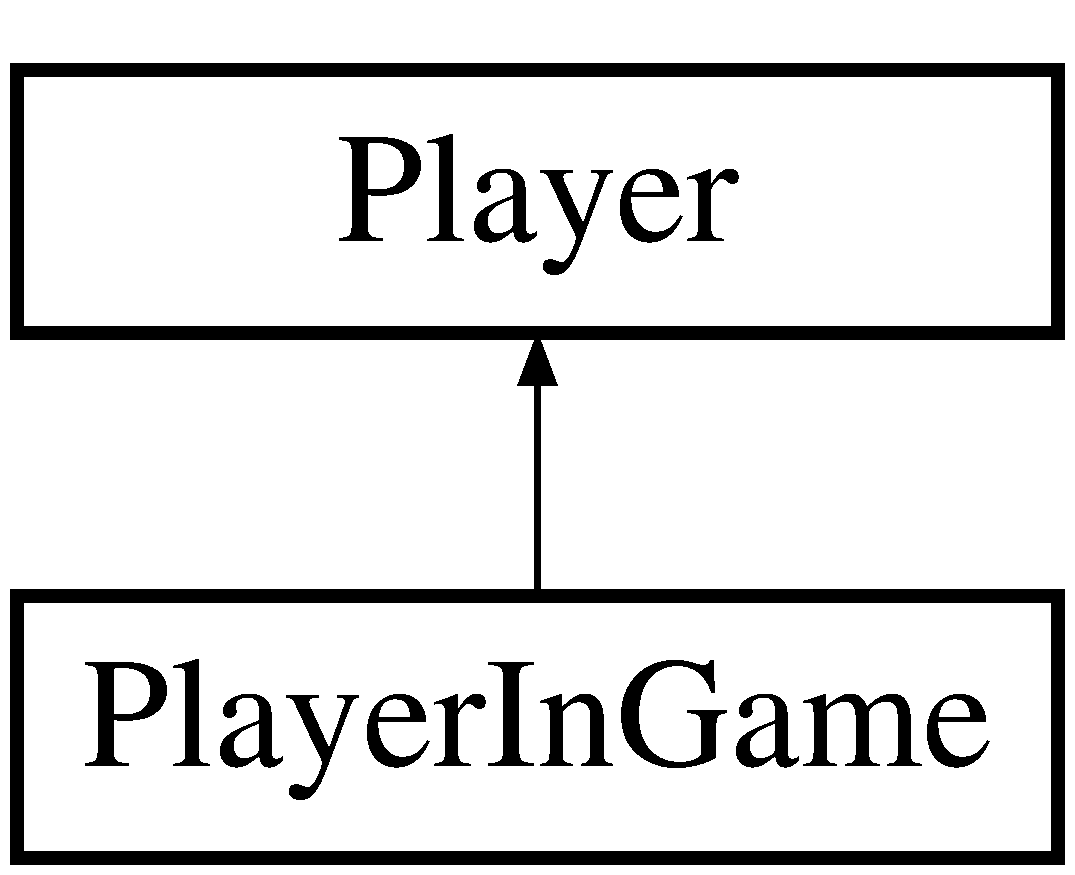
\includegraphics[height=2.000000cm]{classPlayerInGame}
\end{center}
\end{figure}
\subsection*{Fonctions membres publiques}
\begin{DoxyCompactItemize}
\item 
\hyperlink{classPlayerInGame_aef3887730c6e58e3ffa4b8636f5a1fd4}{Player\+In\+Game} ()
\item 
\hyperlink{classPlayerInGame_a64e5c60c2e6106c9dda8c7d79fc36d8b}{Player\+In\+Game} (\hyperlink{classPlayer}{Player} player, \hyperlink{classGame}{Game} $\ast$game)
\item 
\hyperlink{structdataIGPlayer}{data\+I\+G\+Player} \hyperlink{classPlayerInGame_addeeee2e42cf2009fc21511624414146}{get\+Data\+Player} ()
\item 
std\+::vector$<$ \hyperlink{classCardMonster}{Card\+Monster} $\ast$ $>$ \hyperlink{classPlayerInGame_a519fc525decf5af1217b93749cd9ae99}{get\+Cards\+Placed} ()
\item 
unsigned \hyperlink{classPlayerInGame_a9f8df0a2ef00955f318b41149f57fcb7}{nbr\+Card\+In\+Hand} ()
\item 
void \hyperlink{classPlayerInGame_a399370210526407c4234d19815a5fa44}{set\+Deck} (\hyperlink{classDeck}{Deck} $\ast$deck)
\item 
bool \hyperlink{classPlayerInGame_af4d06834c260aebb66c113f397ba3c86}{is\+Deck\+Defined} ()
\item 
void \hyperlink{classPlayerInGame_a646d88b36595c2754ce33555b867c012}{draw} ()
\item 
bool \hyperlink{classPlayerInGame_ac1629d9cadf7445be42eb3245daef6c4}{have\+Enough\+Energy} (\hyperlink{classCard}{Card} $\ast$card)
\item 
void \hyperlink{classPlayerInGame_aedc8c0d75e0d249fde42329dc0a59557}{add\+Max\+Energy} ()
\item 
void \hyperlink{classPlayerInGame_ad18e833fa982d9db29521b49c74b1fa0}{reset\+Energy} ()
\item 
virtual \hyperlink{classPlayerInGame_a75256787f26b0d264a929e61889caba1}{$\sim$\+Player\+In\+Game} ()=default
\end{DoxyCompactItemize}
\subsection*{Membres hérités additionnels}


\subsection{Documentation des constructeurs et destructeur}
\hypertarget{classPlayerInGame_aef3887730c6e58e3ffa4b8636f5a1fd4}{}\index{Player\+In\+Game@{Player\+In\+Game}!Player\+In\+Game@{Player\+In\+Game}}
\index{Player\+In\+Game@{Player\+In\+Game}!Player\+In\+Game@{Player\+In\+Game}}
\subsubsection[{Player\+In\+Game()}]{\setlength{\rightskip}{0pt plus 5cm}Player\+In\+Game\+::\+Player\+In\+Game (
\begin{DoxyParamCaption}
{}
\end{DoxyParamCaption}
)}\label{classPlayerInGame_aef3887730c6e58e3ffa4b8636f5a1fd4}
\hypertarget{classPlayerInGame_a64e5c60c2e6106c9dda8c7d79fc36d8b}{}\index{Player\+In\+Game@{Player\+In\+Game}!Player\+In\+Game@{Player\+In\+Game}}
\index{Player\+In\+Game@{Player\+In\+Game}!Player\+In\+Game@{Player\+In\+Game}}
\subsubsection[{Player\+In\+Game(\+Player player, Game $\ast$game)}]{\setlength{\rightskip}{0pt plus 5cm}Player\+In\+Game\+::\+Player\+In\+Game (
\begin{DoxyParamCaption}
\item[{{\bf Player}}]{player, }
\item[{{\bf Game} $\ast$}]{game}
\end{DoxyParamCaption}
)}\label{classPlayerInGame_a64e5c60c2e6106c9dda8c7d79fc36d8b}
\hypertarget{classPlayerInGame_a75256787f26b0d264a929e61889caba1}{}\index{Player\+In\+Game@{Player\+In\+Game}!````~Player\+In\+Game@{$\sim$\+Player\+In\+Game}}
\index{````~Player\+In\+Game@{$\sim$\+Player\+In\+Game}!Player\+In\+Game@{Player\+In\+Game}}
\subsubsection[{$\sim$\+Player\+In\+Game()=default}]{\setlength{\rightskip}{0pt plus 5cm}virtual Player\+In\+Game\+::$\sim$\+Player\+In\+Game (
\begin{DoxyParamCaption}
{}
\end{DoxyParamCaption}
)\hspace{0.3cm}{\ttfamily [virtual]}, {\ttfamily [default]}}\label{classPlayerInGame_a75256787f26b0d264a929e61889caba1}


\subsection{Documentation des fonctions membres}
\hypertarget{classPlayerInGame_aedc8c0d75e0d249fde42329dc0a59557}{}\index{Player\+In\+Game@{Player\+In\+Game}!add\+Max\+Energy@{add\+Max\+Energy}}
\index{add\+Max\+Energy@{add\+Max\+Energy}!Player\+In\+Game@{Player\+In\+Game}}
\subsubsection[{add\+Max\+Energy()}]{\setlength{\rightskip}{0pt plus 5cm}void Player\+In\+Game\+::add\+Max\+Energy (
\begin{DoxyParamCaption}
{}
\end{DoxyParamCaption}
)}\label{classPlayerInGame_aedc8c0d75e0d249fde42329dc0a59557}
\hypertarget{classPlayerInGame_a646d88b36595c2754ce33555b867c012}{}\index{Player\+In\+Game@{Player\+In\+Game}!draw@{draw}}
\index{draw@{draw}!Player\+In\+Game@{Player\+In\+Game}}
\subsubsection[{draw()}]{\setlength{\rightskip}{0pt plus 5cm}void Player\+In\+Game\+::draw (
\begin{DoxyParamCaption}
{}
\end{DoxyParamCaption}
)}\label{classPlayerInGame_a646d88b36595c2754ce33555b867c012}
Gets random card of deck

\begin{DoxyReturn}{Renvoie}
a random card 
\end{DoxyReturn}
\hypertarget{classPlayerInGame_a519fc525decf5af1217b93749cd9ae99}{}\index{Player\+In\+Game@{Player\+In\+Game}!get\+Cards\+Placed@{get\+Cards\+Placed}}
\index{get\+Cards\+Placed@{get\+Cards\+Placed}!Player\+In\+Game@{Player\+In\+Game}}
\subsubsection[{get\+Cards\+Placed()}]{\setlength{\rightskip}{0pt plus 5cm}std\+::vector$<$ {\bf Card\+Monster} $\ast$ $>$ Player\+In\+Game\+::get\+Cards\+Placed (
\begin{DoxyParamCaption}
{}
\end{DoxyParamCaption}
)}\label{classPlayerInGame_a519fc525decf5af1217b93749cd9ae99}
Returns the placed cards \hypertarget{classPlayerInGame_addeeee2e42cf2009fc21511624414146}{}\index{Player\+In\+Game@{Player\+In\+Game}!get\+Data\+Player@{get\+Data\+Player}}
\index{get\+Data\+Player@{get\+Data\+Player}!Player\+In\+Game@{Player\+In\+Game}}
\subsubsection[{get\+Data\+Player()}]{\setlength{\rightskip}{0pt plus 5cm}{\bf data\+I\+G\+Player} Player\+In\+Game\+::get\+Data\+Player (
\begin{DoxyParamCaption}
{}
\end{DoxyParamCaption}
)}\label{classPlayerInGame_addeeee2e42cf2009fc21511624414146}
Creates a \hyperlink{classPlayerInGame}{Player\+In\+Game} and asks to the player which \hyperlink{classDeck}{Deck} he would like to play with Gets data information from this player to send it


\begin{DoxyParams}{Paramètres}
{\em is\+Turn} & of the current player \\
\hline
\end{DoxyParams}
\hypertarget{classPlayerInGame_ac1629d9cadf7445be42eb3245daef6c4}{}\index{Player\+In\+Game@{Player\+In\+Game}!have\+Enough\+Energy@{have\+Enough\+Energy}}
\index{have\+Enough\+Energy@{have\+Enough\+Energy}!Player\+In\+Game@{Player\+In\+Game}}
\subsubsection[{have\+Enough\+Energy(\+Card $\ast$card)}]{\setlength{\rightskip}{0pt plus 5cm}bool Player\+In\+Game\+::have\+Enough\+Energy (
\begin{DoxyParamCaption}
\item[{{\bf Card} $\ast$}]{card}
\end{DoxyParamCaption}
)}\label{classPlayerInGame_ac1629d9cadf7445be42eb3245daef6c4}
\hypertarget{classPlayerInGame_af4d06834c260aebb66c113f397ba3c86}{}\index{Player\+In\+Game@{Player\+In\+Game}!is\+Deck\+Defined@{is\+Deck\+Defined}}
\index{is\+Deck\+Defined@{is\+Deck\+Defined}!Player\+In\+Game@{Player\+In\+Game}}
\subsubsection[{is\+Deck\+Defined()}]{\setlength{\rightskip}{0pt plus 5cm}bool Player\+In\+Game\+::is\+Deck\+Defined (
\begin{DoxyParamCaption}
{}
\end{DoxyParamCaption}
)}\label{classPlayerInGame_af4d06834c260aebb66c113f397ba3c86}
Checks if the deck of this player is defined

\begin{DoxyReturn}{Renvoie}
True if the deck is defined 
\end{DoxyReturn}
\hypertarget{classPlayerInGame_a9f8df0a2ef00955f318b41149f57fcb7}{}\index{Player\+In\+Game@{Player\+In\+Game}!nbr\+Card\+In\+Hand@{nbr\+Card\+In\+Hand}}
\index{nbr\+Card\+In\+Hand@{nbr\+Card\+In\+Hand}!Player\+In\+Game@{Player\+In\+Game}}
\subsubsection[{nbr\+Card\+In\+Hand()}]{\setlength{\rightskip}{0pt plus 5cm}unsigned Player\+In\+Game\+::nbr\+Card\+In\+Hand (
\begin{DoxyParamCaption}
{}
\end{DoxyParamCaption}
)}\label{classPlayerInGame_a9f8df0a2ef00955f318b41149f57fcb7}
\hypertarget{classPlayerInGame_ad18e833fa982d9db29521b49c74b1fa0}{}\index{Player\+In\+Game@{Player\+In\+Game}!reset\+Energy@{reset\+Energy}}
\index{reset\+Energy@{reset\+Energy}!Player\+In\+Game@{Player\+In\+Game}}
\subsubsection[{reset\+Energy()}]{\setlength{\rightskip}{0pt plus 5cm}void Player\+In\+Game\+::reset\+Energy (
\begin{DoxyParamCaption}
{}
\end{DoxyParamCaption}
)}\label{classPlayerInGame_ad18e833fa982d9db29521b49c74b1fa0}
\hypertarget{classPlayerInGame_a399370210526407c4234d19815a5fa44}{}\index{Player\+In\+Game@{Player\+In\+Game}!set\+Deck@{set\+Deck}}
\index{set\+Deck@{set\+Deck}!Player\+In\+Game@{Player\+In\+Game}}
\subsubsection[{set\+Deck(\+Deck $\ast$deck)}]{\setlength{\rightskip}{0pt plus 5cm}void Player\+In\+Game\+::set\+Deck (
\begin{DoxyParamCaption}
\item[{{\bf Deck} $\ast$}]{deck}
\end{DoxyParamCaption}
)}\label{classPlayerInGame_a399370210526407c4234d19815a5fa44}
Sets the player deck and notify it at the game object


\begin{DoxyParams}{Paramètres}
{\em deck} & The selected deck \\
\hline
\end{DoxyParams}


La documentation de cette classe a été générée à partir des fichiers suivants \+:\begin{DoxyCompactItemize}
\item 
server/\hyperlink{PlayerInGame_8hpp}{Player\+In\+Game.\+hpp}\item 
server/\hyperlink{PlayerInGame_8cpp}{Player\+In\+Game.\+cpp}\end{DoxyCompactItemize}

\hypertarget{classPlayerManager}{}\section{Référence de la classe Player\+Manager}
\label{classPlayerManager}\index{Player\+Manager@{Player\+Manager}}


{\ttfamily \#include $<$Player\+Manager.\+hpp$>$}

\subsection*{Fonctions membres publiques}
\begin{DoxyCompactItemize}
\item 
\hyperlink{classPlayerManager_a203221ed2aaa70c55832fe82738f6f7e}{Player\+Manager} ()=default
\item 
std\+::string \hyperlink{classPlayerManager_a01bdeb0501e0e96afed4818c58443657}{get\+Ranking} ()
\item 
void \hyperlink{classPlayerManager_a85e370f3ac930bf829ca807ea992f4b5}{load\+Players} ()
\item 
void \hyperlink{classPlayerManager_af260b18463c9244e5f826cd200306714}{save\+Players} () const 
\item 
\hyperlink{classPlayer}{Player} $\ast$ \hyperlink{classPlayerManager_acb14cf0559b1d199045898d959740788}{sign\+Up} (std\+::string, std\+::string, int)
\item 
\hyperlink{classPlayer}{Player} $\ast$ \hyperlink{classPlayerManager_a4cfd0c1c7269de24cb8c150f43d92752}{log\+In} (std\+::string, std\+::string, int)
\item 
virtual \hyperlink{classPlayerManager_a92841310f064ebaed59ffde6620216dc}{$\sim$\+Player\+Manager} ()=default
\end{DoxyCompactItemize}


\subsection{Documentation des constructeurs et destructeur}
\hypertarget{classPlayerManager_a203221ed2aaa70c55832fe82738f6f7e}{}\index{Player\+Manager@{Player\+Manager}!Player\+Manager@{Player\+Manager}}
\index{Player\+Manager@{Player\+Manager}!Player\+Manager@{Player\+Manager}}
\subsubsection[{Player\+Manager()=default}]{\setlength{\rightskip}{0pt plus 5cm}Player\+Manager\+::\+Player\+Manager (
\begin{DoxyParamCaption}
{}
\end{DoxyParamCaption}
)\hspace{0.3cm}{\ttfamily [default]}}\label{classPlayerManager_a203221ed2aaa70c55832fe82738f6f7e}
\hypertarget{classPlayerManager_a92841310f064ebaed59ffde6620216dc}{}\index{Player\+Manager@{Player\+Manager}!````~Player\+Manager@{$\sim$\+Player\+Manager}}
\index{````~Player\+Manager@{$\sim$\+Player\+Manager}!Player\+Manager@{Player\+Manager}}
\subsubsection[{$\sim$\+Player\+Manager()=default}]{\setlength{\rightskip}{0pt plus 5cm}virtual Player\+Manager\+::$\sim$\+Player\+Manager (
\begin{DoxyParamCaption}
{}
\end{DoxyParamCaption}
)\hspace{0.3cm}{\ttfamily [virtual]}, {\ttfamily [default]}}\label{classPlayerManager_a92841310f064ebaed59ffde6620216dc}


\subsection{Documentation des fonctions membres}
\hypertarget{classPlayerManager_a01bdeb0501e0e96afed4818c58443657}{}\index{Player\+Manager@{Player\+Manager}!get\+Ranking@{get\+Ranking}}
\index{get\+Ranking@{get\+Ranking}!Player\+Manager@{Player\+Manager}}
\subsubsection[{get\+Ranking()}]{\setlength{\rightskip}{0pt plus 5cm}std\+::string Player\+Manager\+::get\+Ranking (
\begin{DoxyParamCaption}
{}
\end{DoxyParamCaption}
)}\label{classPlayerManager_a01bdeb0501e0e96afed4818c58443657}
\hypertarget{classPlayerManager_a85e370f3ac930bf829ca807ea992f4b5}{}\index{Player\+Manager@{Player\+Manager}!load\+Players@{load\+Players}}
\index{load\+Players@{load\+Players}!Player\+Manager@{Player\+Manager}}
\subsubsection[{load\+Players()}]{\setlength{\rightskip}{0pt plus 5cm}void Player\+Manager\+::load\+Players (
\begin{DoxyParamCaption}
{}
\end{DoxyParamCaption}
)}\label{classPlayerManager_a85e370f3ac930bf829ca807ea992f4b5}
\hypertarget{classPlayerManager_a4cfd0c1c7269de24cb8c150f43d92752}{}\index{Player\+Manager@{Player\+Manager}!log\+In@{log\+In}}
\index{log\+In@{log\+In}!Player\+Manager@{Player\+Manager}}
\subsubsection[{log\+In(std\+::string, std\+::string, int)}]{\setlength{\rightskip}{0pt plus 5cm}{\bf Player} $\ast$ Player\+Manager\+::log\+In (
\begin{DoxyParamCaption}
\item[{std\+::string}]{username, }
\item[{std\+::string}]{password, }
\item[{int}]{sockfd}
\end{DoxyParamCaption}
)}\label{classPlayerManager_a4cfd0c1c7269de24cb8c150f43d92752}
\hypertarget{classPlayerManager_af260b18463c9244e5f826cd200306714}{}\index{Player\+Manager@{Player\+Manager}!save\+Players@{save\+Players}}
\index{save\+Players@{save\+Players}!Player\+Manager@{Player\+Manager}}
\subsubsection[{save\+Players() const }]{\setlength{\rightskip}{0pt plus 5cm}void Player\+Manager\+::save\+Players (
\begin{DoxyParamCaption}
{}
\end{DoxyParamCaption}
) const}\label{classPlayerManager_af260b18463c9244e5f826cd200306714}
\hypertarget{classPlayerManager_acb14cf0559b1d199045898d959740788}{}\index{Player\+Manager@{Player\+Manager}!sign\+Up@{sign\+Up}}
\index{sign\+Up@{sign\+Up}!Player\+Manager@{Player\+Manager}}
\subsubsection[{sign\+Up(std\+::string, std\+::string, int)}]{\setlength{\rightskip}{0pt plus 5cm}{\bf Player} $\ast$ Player\+Manager\+::sign\+Up (
\begin{DoxyParamCaption}
\item[{std\+::string}]{username, }
\item[{std\+::string}]{password, }
\item[{int}]{sockfd}
\end{DoxyParamCaption}
)}\label{classPlayerManager_acb14cf0559b1d199045898d959740788}


La documentation de cette classe a été générée à partir des fichiers suivants \+:\begin{DoxyCompactItemize}
\item 
server/\hyperlink{PlayerManager_8hpp}{Player\+Manager.\+hpp}\item 
server/\hyperlink{PlayerManager_8cpp}{Player\+Manager.\+cpp}\end{DoxyCompactItemize}

\chapter{Documentation des fichiers}
\hypertarget{Board_8hpp}{}\section{Référence du fichier client/\+Board.hpp}
\label{Board_8hpp}\index{client/\+Board.\+hpp@{client/\+Board.\+hpp}}
\subsection*{Classes}
\begin{DoxyCompactItemize}
\item 
class \hyperlink{classBoard}{Board}
\end{DoxyCompactItemize}

\hypertarget{client_2Card_8hpp}{}\section{Référence du fichier client/\+Card.hpp}
\label{client_2Card_8hpp}\index{client/\+Card.\+hpp@{client/\+Card.\+hpp}}
{\ttfamily \#include $<$string$>$}\\*
\subsection*{Classes}
\begin{DoxyCompactItemize}
\item 
class \hyperlink{classCard}{Card}
\end{DoxyCompactItemize}

\hypertarget{server_2Card_8hpp}{}\section{Référence du fichier server/\+Card.hpp}
\label{server_2Card_8hpp}\index{server/\+Card.\+hpp@{server/\+Card.\+hpp}}
{\ttfamily \#include $<$string$>$}\\*
{\ttfamily \#include $<$map$>$}\\*
{\ttfamily \#include $<$cstddef$>$}\\*
{\ttfamily \#include \char`\"{}Effect.\+hpp\char`\"{}}\\*
\subsection*{Classes}
\begin{DoxyCompactItemize}
\item 
class \hyperlink{classCard}{Card}
\end{DoxyCompactItemize}

\hypertarget{Classement_8hpp}{}\section{Référence du fichier client/\+Classement.hpp}
\label{Classement_8hpp}\index{client/\+Classement.\+hpp@{client/\+Classement.\+hpp}}
\subsection*{Classes}
\begin{DoxyCompactItemize}
\item 
class \hyperlink{classClassement}{Classement}
\end{DoxyCompactItemize}

\hypertarget{CLI_8cpp}{}\section{Référence du fichier client/\+C\+L\+I.cpp}
\label{CLI_8cpp}\index{client/\+C\+L\+I.\+cpp@{client/\+C\+L\+I.\+cpp}}
{\ttfamily \#include \char`\"{}C\+L\+I.\+hpp\char`\"{}}\\*

\hypertarget{CLI_8hpp}{}\section{Référence du fichier client/\+C\+L\+I.hpp}
\label{CLI_8hpp}\index{client/\+C\+L\+I.\+hpp@{client/\+C\+L\+I.\+hpp}}
{\ttfamily \#include $<$ncurses.\+h$>$}\\*
{\ttfamily \#include $<$panel.\+h$>$}\\*
{\ttfamily \#include $<$string$>$}\\*
{\ttfamily \#include \char`\"{}common/\+Wizard\+Logger.\+hpp\char`\"{}}\\*
{\ttfamily \#include \char`\"{}Display.\+hpp\char`\"{}}\\*
{\ttfamily \#include \char`\"{}client/\+C\+L\+I/\+C\+L\+I\+Panel.\+hpp\char`\"{}}\\*
{\ttfamily \#include \char`\"{}client/\+C\+L\+I/\+Login\+Panel.\+hpp\char`\"{}}\\*
{\ttfamily \#include \char`\"{}client/\+C\+L\+I/\+Main\+Panel.\+hpp\char`\"{}}\\*
\subsection*{Classes}
\begin{DoxyCompactItemize}
\item 
class \hyperlink{classCLI}{C\+L\+I}
\end{DoxyCompactItemize}
\subsection*{Macros}
\begin{DoxyCompactItemize}
\item 
\#define \hyperlink{CLI_8hpp_a5c16299dfdf0a77b186ce91c8063bdb9}{D\+E\+F\+A\+U\+L\+T\+\_\+\+E\+M\+P\+T\+Y\+\_\+\+S\+P\+A\+C\+E}~2
\item 
\#define \hyperlink{CLI_8hpp_a321ae946de24c36489276616d13c46cd}{L\+I\+N\+E\+S}~37
\item 
\#define \hyperlink{CLI_8hpp_a628405768f066e7a73900678e622770c}{C\+O\+L\+L\+O\+N\+N\+E\+S}~96
\item 
\#define \hyperlink{CLI_8hpp_a0aebff1da224d1b5d3e8e8d7d41300ec}{C\+O\+M\+M\+A\+N\+D\+E\+\_\+\+P\+A\+N\+E\+L\+\_\+\+H\+E\+I\+G\+T\+H}~1
\item 
\#define \hyperlink{CLI_8hpp_a1022328666447f08e6841e68f93db36b}{G\+A\+M\+E\+\_\+\+H\+E\+I\+G\+T\+H}~21
\item 
\#define \hyperlink{CLI_8hpp_a693f306b88f7336281e4d1f07754579c}{G\+A\+M\+E\+\_\+\+W\+I\+D\+T\+H}~63
\item 
\#define \hyperlink{CLI_8hpp_ac9ff64cd26da3bb271e42ce913aebe82}{C\+A\+R\+D\+\_\+\+H\+E\+I\+G\+T\+H}~(\hyperlink{CLI_8hpp_a1022328666447f08e6841e68f93db36b}{G\+A\+M\+E\+\_\+\+H\+E\+I\+G\+T\+H}\%3)
\item 
\#define \hyperlink{CLI_8hpp_ad6ff324701f28fdcd04a8408f68a3f6c}{C\+A\+R\+D\+\_\+\+W\+I\+D\+T\+H}~(\hyperlink{CLI_8hpp_a693f306b88f7336281e4d1f07754579c}{G\+A\+M\+E\+\_\+\+W\+I\+D\+T\+H}\%7)
\item 
\#define \hyperlink{CLI_8hpp_a97f6acaad01fed1c09886eac51f361db}{P\+L\+A\+Y\+E\+R\+\_\+\+I\+N\+F\+O\+\_\+\+H\+E\+I\+G\+T\+H}~(3+2$\ast$\hyperlink{CLI_8hpp_a5c16299dfdf0a77b186ce91c8063bdb9}{D\+E\+F\+A\+U\+L\+T\+\_\+\+E\+M\+P\+T\+Y\+\_\+\+S\+P\+A\+C\+E})
\item 
\#define \hyperlink{CLI_8hpp_a2f9f5939f8bbd2dc6365efdb99aacb83}{P\+L\+A\+Y\+E\+R\+\_\+\+I\+N\+F\+O\+\_\+\+W\+I\+D\+T\+H}~\hyperlink{CLI_8hpp_a693f306b88f7336281e4d1f07754579c}{G\+A\+M\+E\+\_\+\+W\+I\+D\+T\+H}
\item 
\#define \hyperlink{CLI_8hpp_aff8fff0c2f56d7c64318738a596e0387}{T\+C\+H\+A\+T\+\_\+\+I\+N\+P\+U\+T\+\_\+\+H\+E\+I\+G\+T\+H}~\hyperlink{CLI_8hpp_a97f6acaad01fed1c09886eac51f361db}{P\+L\+A\+Y\+E\+R\+\_\+\+I\+N\+F\+O\+\_\+\+H\+E\+I\+G\+T\+H}
\item 
\#define \hyperlink{CLI_8hpp_ab8b1f21cb0908481707de677bf3bb596}{T\+C\+H\+A\+T\+\_\+\+I\+N\+P\+U\+T\+\_\+\+W\+I\+D\+T\+H}~27
\item 
\#define \hyperlink{CLI_8hpp_a660ed6f3a09f7f39be7913f8496191ce}{T\+C\+H\+A\+T\+\_\+\+H\+E\+I\+G\+T\+H}~14
\item 
\#define \hyperlink{CLI_8hpp_a63d094e74ed0640235cbfc26479e3706}{T\+C\+H\+A\+T\+\_\+\+W\+I\+D\+T\+H}~\hyperlink{CLI_8hpp_ab8b1f21cb0908481707de677bf3bb596}{T\+C\+H\+A\+T\+\_\+\+I\+N\+P\+U\+T\+\_\+\+W\+I\+D\+T\+H}
\item 
\#define \hyperlink{CLI_8hpp_abc246160f0fd6108f7045c098f5f500f}{C\+A\+R\+D\+\_\+\+I\+N\+F\+O\+\_\+\+H\+E\+I\+G\+T\+H}~5
\item 
\#define \hyperlink{CLI_8hpp_a9621c1a5a13bee3200fb686675869d8b}{C\+A\+R\+D\+\_\+\+I\+N\+F\+O\+\_\+\+W\+I\+D\+T\+H}~\hyperlink{CLI_8hpp_ab8b1f21cb0908481707de677bf3bb596}{T\+C\+H\+A\+T\+\_\+\+I\+N\+P\+U\+T\+\_\+\+W\+I\+D\+T\+H}
\item 
\#define \hyperlink{CLI_8hpp_a32db537bbe2f7a59c1c17ea2ad081f36}{P\+A\+N\+E\+L\+\_\+\+T\+O\+T\+A\+L\+\_\+\+N\+U\+M\+B\+E\+R}~1
\end{DoxyCompactItemize}


\subsection{Documentation des macros}
\hypertarget{CLI_8hpp_ac9ff64cd26da3bb271e42ce913aebe82}{}\index{C\+L\+I.\+hpp@{C\+L\+I.\+hpp}!C\+A\+R\+D\+\_\+\+H\+E\+I\+G\+T\+H@{C\+A\+R\+D\+\_\+\+H\+E\+I\+G\+T\+H}}
\index{C\+A\+R\+D\+\_\+\+H\+E\+I\+G\+T\+H@{C\+A\+R\+D\+\_\+\+H\+E\+I\+G\+T\+H}!C\+L\+I.\+hpp@{C\+L\+I.\+hpp}}
\subsubsection[{C\+A\+R\+D\+\_\+\+H\+E\+I\+G\+T\+H}]{\setlength{\rightskip}{0pt plus 5cm}\#define C\+A\+R\+D\+\_\+\+H\+E\+I\+G\+T\+H~({\bf G\+A\+M\+E\+\_\+\+H\+E\+I\+G\+T\+H}\%3)}\label{CLI_8hpp_ac9ff64cd26da3bb271e42ce913aebe82}
\hypertarget{CLI_8hpp_abc246160f0fd6108f7045c098f5f500f}{}\index{C\+L\+I.\+hpp@{C\+L\+I.\+hpp}!C\+A\+R\+D\+\_\+\+I\+N\+F\+O\+\_\+\+H\+E\+I\+G\+T\+H@{C\+A\+R\+D\+\_\+\+I\+N\+F\+O\+\_\+\+H\+E\+I\+G\+T\+H}}
\index{C\+A\+R\+D\+\_\+\+I\+N\+F\+O\+\_\+\+H\+E\+I\+G\+T\+H@{C\+A\+R\+D\+\_\+\+I\+N\+F\+O\+\_\+\+H\+E\+I\+G\+T\+H}!C\+L\+I.\+hpp@{C\+L\+I.\+hpp}}
\subsubsection[{C\+A\+R\+D\+\_\+\+I\+N\+F\+O\+\_\+\+H\+E\+I\+G\+T\+H}]{\setlength{\rightskip}{0pt plus 5cm}\#define C\+A\+R\+D\+\_\+\+I\+N\+F\+O\+\_\+\+H\+E\+I\+G\+T\+H~5}\label{CLI_8hpp_abc246160f0fd6108f7045c098f5f500f}
\hypertarget{CLI_8hpp_a9621c1a5a13bee3200fb686675869d8b}{}\index{C\+L\+I.\+hpp@{C\+L\+I.\+hpp}!C\+A\+R\+D\+\_\+\+I\+N\+F\+O\+\_\+\+W\+I\+D\+T\+H@{C\+A\+R\+D\+\_\+\+I\+N\+F\+O\+\_\+\+W\+I\+D\+T\+H}}
\index{C\+A\+R\+D\+\_\+\+I\+N\+F\+O\+\_\+\+W\+I\+D\+T\+H@{C\+A\+R\+D\+\_\+\+I\+N\+F\+O\+\_\+\+W\+I\+D\+T\+H}!C\+L\+I.\+hpp@{C\+L\+I.\+hpp}}
\subsubsection[{C\+A\+R\+D\+\_\+\+I\+N\+F\+O\+\_\+\+W\+I\+D\+T\+H}]{\setlength{\rightskip}{0pt plus 5cm}\#define C\+A\+R\+D\+\_\+\+I\+N\+F\+O\+\_\+\+W\+I\+D\+T\+H~{\bf T\+C\+H\+A\+T\+\_\+\+I\+N\+P\+U\+T\+\_\+\+W\+I\+D\+T\+H}}\label{CLI_8hpp_a9621c1a5a13bee3200fb686675869d8b}
\hypertarget{CLI_8hpp_ad6ff324701f28fdcd04a8408f68a3f6c}{}\index{C\+L\+I.\+hpp@{C\+L\+I.\+hpp}!C\+A\+R\+D\+\_\+\+W\+I\+D\+T\+H@{C\+A\+R\+D\+\_\+\+W\+I\+D\+T\+H}}
\index{C\+A\+R\+D\+\_\+\+W\+I\+D\+T\+H@{C\+A\+R\+D\+\_\+\+W\+I\+D\+T\+H}!C\+L\+I.\+hpp@{C\+L\+I.\+hpp}}
\subsubsection[{C\+A\+R\+D\+\_\+\+W\+I\+D\+T\+H}]{\setlength{\rightskip}{0pt plus 5cm}\#define C\+A\+R\+D\+\_\+\+W\+I\+D\+T\+H~({\bf G\+A\+M\+E\+\_\+\+W\+I\+D\+T\+H}\%7)}\label{CLI_8hpp_ad6ff324701f28fdcd04a8408f68a3f6c}
\hypertarget{CLI_8hpp_a628405768f066e7a73900678e622770c}{}\index{C\+L\+I.\+hpp@{C\+L\+I.\+hpp}!C\+O\+L\+L\+O\+N\+N\+E\+S@{C\+O\+L\+L\+O\+N\+N\+E\+S}}
\index{C\+O\+L\+L\+O\+N\+N\+E\+S@{C\+O\+L\+L\+O\+N\+N\+E\+S}!C\+L\+I.\+hpp@{C\+L\+I.\+hpp}}
\subsubsection[{C\+O\+L\+L\+O\+N\+N\+E\+S}]{\setlength{\rightskip}{0pt plus 5cm}\#define C\+O\+L\+L\+O\+N\+N\+E\+S~96}\label{CLI_8hpp_a628405768f066e7a73900678e622770c}
\hypertarget{CLI_8hpp_a0aebff1da224d1b5d3e8e8d7d41300ec}{}\index{C\+L\+I.\+hpp@{C\+L\+I.\+hpp}!C\+O\+M\+M\+A\+N\+D\+E\+\_\+\+P\+A\+N\+E\+L\+\_\+\+H\+E\+I\+G\+T\+H@{C\+O\+M\+M\+A\+N\+D\+E\+\_\+\+P\+A\+N\+E\+L\+\_\+\+H\+E\+I\+G\+T\+H}}
\index{C\+O\+M\+M\+A\+N\+D\+E\+\_\+\+P\+A\+N\+E\+L\+\_\+\+H\+E\+I\+G\+T\+H@{C\+O\+M\+M\+A\+N\+D\+E\+\_\+\+P\+A\+N\+E\+L\+\_\+\+H\+E\+I\+G\+T\+H}!C\+L\+I.\+hpp@{C\+L\+I.\+hpp}}
\subsubsection[{C\+O\+M\+M\+A\+N\+D\+E\+\_\+\+P\+A\+N\+E\+L\+\_\+\+H\+E\+I\+G\+T\+H}]{\setlength{\rightskip}{0pt plus 5cm}\#define C\+O\+M\+M\+A\+N\+D\+E\+\_\+\+P\+A\+N\+E\+L\+\_\+\+H\+E\+I\+G\+T\+H~1}\label{CLI_8hpp_a0aebff1da224d1b5d3e8e8d7d41300ec}
\hypertarget{CLI_8hpp_a5c16299dfdf0a77b186ce91c8063bdb9}{}\index{C\+L\+I.\+hpp@{C\+L\+I.\+hpp}!D\+E\+F\+A\+U\+L\+T\+\_\+\+E\+M\+P\+T\+Y\+\_\+\+S\+P\+A\+C\+E@{D\+E\+F\+A\+U\+L\+T\+\_\+\+E\+M\+P\+T\+Y\+\_\+\+S\+P\+A\+C\+E}}
\index{D\+E\+F\+A\+U\+L\+T\+\_\+\+E\+M\+P\+T\+Y\+\_\+\+S\+P\+A\+C\+E@{D\+E\+F\+A\+U\+L\+T\+\_\+\+E\+M\+P\+T\+Y\+\_\+\+S\+P\+A\+C\+E}!C\+L\+I.\+hpp@{C\+L\+I.\+hpp}}
\subsubsection[{D\+E\+F\+A\+U\+L\+T\+\_\+\+E\+M\+P\+T\+Y\+\_\+\+S\+P\+A\+C\+E}]{\setlength{\rightskip}{0pt plus 5cm}\#define D\+E\+F\+A\+U\+L\+T\+\_\+\+E\+M\+P\+T\+Y\+\_\+\+S\+P\+A\+C\+E~2}\label{CLI_8hpp_a5c16299dfdf0a77b186ce91c8063bdb9}
in-\/game layout \subparagraph*{}

\subsection*{}

\subsection*{\# \# card\+Info}

\subsection*{}

\subsection*{}

\subsection*{}

\subsection*{}

\subsection*{}

\subsection*{game\+Panel}

\subsection*{\# \# tchat}

\subsection*{}

\subsection*{}

\subsection*{}

\subparagraph*{}

\subparagraph*{}

\subsection*{\# \# tchat}

\subsection*{players\+Info \# \# input}

\subparagraph*{}

\subparagraph*{}

\subsection*{command\+List (key shortcut)}

\subparagraph*{}\hypertarget{CLI_8hpp_a1022328666447f08e6841e68f93db36b}{}\index{C\+L\+I.\+hpp@{C\+L\+I.\+hpp}!G\+A\+M\+E\+\_\+\+H\+E\+I\+G\+T\+H@{G\+A\+M\+E\+\_\+\+H\+E\+I\+G\+T\+H}}
\index{G\+A\+M\+E\+\_\+\+H\+E\+I\+G\+T\+H@{G\+A\+M\+E\+\_\+\+H\+E\+I\+G\+T\+H}!C\+L\+I.\+hpp@{C\+L\+I.\+hpp}}
\subsubsection[{G\+A\+M\+E\+\_\+\+H\+E\+I\+G\+T\+H}]{\setlength{\rightskip}{0pt plus 5cm}\#define G\+A\+M\+E\+\_\+\+H\+E\+I\+G\+T\+H~21}\label{CLI_8hpp_a1022328666447f08e6841e68f93db36b}
\hypertarget{CLI_8hpp_a693f306b88f7336281e4d1f07754579c}{}\index{C\+L\+I.\+hpp@{C\+L\+I.\+hpp}!G\+A\+M\+E\+\_\+\+W\+I\+D\+T\+H@{G\+A\+M\+E\+\_\+\+W\+I\+D\+T\+H}}
\index{G\+A\+M\+E\+\_\+\+W\+I\+D\+T\+H@{G\+A\+M\+E\+\_\+\+W\+I\+D\+T\+H}!C\+L\+I.\+hpp@{C\+L\+I.\+hpp}}
\subsubsection[{G\+A\+M\+E\+\_\+\+W\+I\+D\+T\+H}]{\setlength{\rightskip}{0pt plus 5cm}\#define G\+A\+M\+E\+\_\+\+W\+I\+D\+T\+H~63}\label{CLI_8hpp_a693f306b88f7336281e4d1f07754579c}
\hypertarget{CLI_8hpp_a321ae946de24c36489276616d13c46cd}{}\index{C\+L\+I.\+hpp@{C\+L\+I.\+hpp}!L\+I\+N\+E\+S@{L\+I\+N\+E\+S}}
\index{L\+I\+N\+E\+S@{L\+I\+N\+E\+S}!C\+L\+I.\+hpp@{C\+L\+I.\+hpp}}
\subsubsection[{L\+I\+N\+E\+S}]{\setlength{\rightskip}{0pt plus 5cm}\#define L\+I\+N\+E\+S~37}\label{CLI_8hpp_a321ae946de24c36489276616d13c46cd}
\hypertarget{CLI_8hpp_a32db537bbe2f7a59c1c17ea2ad081f36}{}\index{C\+L\+I.\+hpp@{C\+L\+I.\+hpp}!P\+A\+N\+E\+L\+\_\+\+T\+O\+T\+A\+L\+\_\+\+N\+U\+M\+B\+E\+R@{P\+A\+N\+E\+L\+\_\+\+T\+O\+T\+A\+L\+\_\+\+N\+U\+M\+B\+E\+R}}
\index{P\+A\+N\+E\+L\+\_\+\+T\+O\+T\+A\+L\+\_\+\+N\+U\+M\+B\+E\+R@{P\+A\+N\+E\+L\+\_\+\+T\+O\+T\+A\+L\+\_\+\+N\+U\+M\+B\+E\+R}!C\+L\+I.\+hpp@{C\+L\+I.\+hpp}}
\subsubsection[{P\+A\+N\+E\+L\+\_\+\+T\+O\+T\+A\+L\+\_\+\+N\+U\+M\+B\+E\+R}]{\setlength{\rightskip}{0pt plus 5cm}\#define P\+A\+N\+E\+L\+\_\+\+T\+O\+T\+A\+L\+\_\+\+N\+U\+M\+B\+E\+R~1}\label{CLI_8hpp_a32db537bbe2f7a59c1c17ea2ad081f36}
\hypertarget{CLI_8hpp_a97f6acaad01fed1c09886eac51f361db}{}\index{C\+L\+I.\+hpp@{C\+L\+I.\+hpp}!P\+L\+A\+Y\+E\+R\+\_\+\+I\+N\+F\+O\+\_\+\+H\+E\+I\+G\+T\+H@{P\+L\+A\+Y\+E\+R\+\_\+\+I\+N\+F\+O\+\_\+\+H\+E\+I\+G\+T\+H}}
\index{P\+L\+A\+Y\+E\+R\+\_\+\+I\+N\+F\+O\+\_\+\+H\+E\+I\+G\+T\+H@{P\+L\+A\+Y\+E\+R\+\_\+\+I\+N\+F\+O\+\_\+\+H\+E\+I\+G\+T\+H}!C\+L\+I.\+hpp@{C\+L\+I.\+hpp}}
\subsubsection[{P\+L\+A\+Y\+E\+R\+\_\+\+I\+N\+F\+O\+\_\+\+H\+E\+I\+G\+T\+H}]{\setlength{\rightskip}{0pt plus 5cm}\#define P\+L\+A\+Y\+E\+R\+\_\+\+I\+N\+F\+O\+\_\+\+H\+E\+I\+G\+T\+H~(3+2$\ast${\bf D\+E\+F\+A\+U\+L\+T\+\_\+\+E\+M\+P\+T\+Y\+\_\+\+S\+P\+A\+C\+E})}\label{CLI_8hpp_a97f6acaad01fed1c09886eac51f361db}
\hypertarget{CLI_8hpp_a2f9f5939f8bbd2dc6365efdb99aacb83}{}\index{C\+L\+I.\+hpp@{C\+L\+I.\+hpp}!P\+L\+A\+Y\+E\+R\+\_\+\+I\+N\+F\+O\+\_\+\+W\+I\+D\+T\+H@{P\+L\+A\+Y\+E\+R\+\_\+\+I\+N\+F\+O\+\_\+\+W\+I\+D\+T\+H}}
\index{P\+L\+A\+Y\+E\+R\+\_\+\+I\+N\+F\+O\+\_\+\+W\+I\+D\+T\+H@{P\+L\+A\+Y\+E\+R\+\_\+\+I\+N\+F\+O\+\_\+\+W\+I\+D\+T\+H}!C\+L\+I.\+hpp@{C\+L\+I.\+hpp}}
\subsubsection[{P\+L\+A\+Y\+E\+R\+\_\+\+I\+N\+F\+O\+\_\+\+W\+I\+D\+T\+H}]{\setlength{\rightskip}{0pt plus 5cm}\#define P\+L\+A\+Y\+E\+R\+\_\+\+I\+N\+F\+O\+\_\+\+W\+I\+D\+T\+H~{\bf G\+A\+M\+E\+\_\+\+W\+I\+D\+T\+H}}\label{CLI_8hpp_a2f9f5939f8bbd2dc6365efdb99aacb83}
\hypertarget{CLI_8hpp_a660ed6f3a09f7f39be7913f8496191ce}{}\index{C\+L\+I.\+hpp@{C\+L\+I.\+hpp}!T\+C\+H\+A\+T\+\_\+\+H\+E\+I\+G\+T\+H@{T\+C\+H\+A\+T\+\_\+\+H\+E\+I\+G\+T\+H}}
\index{T\+C\+H\+A\+T\+\_\+\+H\+E\+I\+G\+T\+H@{T\+C\+H\+A\+T\+\_\+\+H\+E\+I\+G\+T\+H}!C\+L\+I.\+hpp@{C\+L\+I.\+hpp}}
\subsubsection[{T\+C\+H\+A\+T\+\_\+\+H\+E\+I\+G\+T\+H}]{\setlength{\rightskip}{0pt plus 5cm}\#define T\+C\+H\+A\+T\+\_\+\+H\+E\+I\+G\+T\+H~14}\label{CLI_8hpp_a660ed6f3a09f7f39be7913f8496191ce}
\hypertarget{CLI_8hpp_aff8fff0c2f56d7c64318738a596e0387}{}\index{C\+L\+I.\+hpp@{C\+L\+I.\+hpp}!T\+C\+H\+A\+T\+\_\+\+I\+N\+P\+U\+T\+\_\+\+H\+E\+I\+G\+T\+H@{T\+C\+H\+A\+T\+\_\+\+I\+N\+P\+U\+T\+\_\+\+H\+E\+I\+G\+T\+H}}
\index{T\+C\+H\+A\+T\+\_\+\+I\+N\+P\+U\+T\+\_\+\+H\+E\+I\+G\+T\+H@{T\+C\+H\+A\+T\+\_\+\+I\+N\+P\+U\+T\+\_\+\+H\+E\+I\+G\+T\+H}!C\+L\+I.\+hpp@{C\+L\+I.\+hpp}}
\subsubsection[{T\+C\+H\+A\+T\+\_\+\+I\+N\+P\+U\+T\+\_\+\+H\+E\+I\+G\+T\+H}]{\setlength{\rightskip}{0pt plus 5cm}\#define T\+C\+H\+A\+T\+\_\+\+I\+N\+P\+U\+T\+\_\+\+H\+E\+I\+G\+T\+H~{\bf P\+L\+A\+Y\+E\+R\+\_\+\+I\+N\+F\+O\+\_\+\+H\+E\+I\+G\+T\+H}}\label{CLI_8hpp_aff8fff0c2f56d7c64318738a596e0387}
\hypertarget{CLI_8hpp_ab8b1f21cb0908481707de677bf3bb596}{}\index{C\+L\+I.\+hpp@{C\+L\+I.\+hpp}!T\+C\+H\+A\+T\+\_\+\+I\+N\+P\+U\+T\+\_\+\+W\+I\+D\+T\+H@{T\+C\+H\+A\+T\+\_\+\+I\+N\+P\+U\+T\+\_\+\+W\+I\+D\+T\+H}}
\index{T\+C\+H\+A\+T\+\_\+\+I\+N\+P\+U\+T\+\_\+\+W\+I\+D\+T\+H@{T\+C\+H\+A\+T\+\_\+\+I\+N\+P\+U\+T\+\_\+\+W\+I\+D\+T\+H}!C\+L\+I.\+hpp@{C\+L\+I.\+hpp}}
\subsubsection[{T\+C\+H\+A\+T\+\_\+\+I\+N\+P\+U\+T\+\_\+\+W\+I\+D\+T\+H}]{\setlength{\rightskip}{0pt plus 5cm}\#define T\+C\+H\+A\+T\+\_\+\+I\+N\+P\+U\+T\+\_\+\+W\+I\+D\+T\+H~27}\label{CLI_8hpp_ab8b1f21cb0908481707de677bf3bb596}
\hypertarget{CLI_8hpp_a63d094e74ed0640235cbfc26479e3706}{}\index{C\+L\+I.\+hpp@{C\+L\+I.\+hpp}!T\+C\+H\+A\+T\+\_\+\+W\+I\+D\+T\+H@{T\+C\+H\+A\+T\+\_\+\+W\+I\+D\+T\+H}}
\index{T\+C\+H\+A\+T\+\_\+\+W\+I\+D\+T\+H@{T\+C\+H\+A\+T\+\_\+\+W\+I\+D\+T\+H}!C\+L\+I.\+hpp@{C\+L\+I.\+hpp}}
\subsubsection[{T\+C\+H\+A\+T\+\_\+\+W\+I\+D\+T\+H}]{\setlength{\rightskip}{0pt plus 5cm}\#define T\+C\+H\+A\+T\+\_\+\+W\+I\+D\+T\+H~{\bf T\+C\+H\+A\+T\+\_\+\+I\+N\+P\+U\+T\+\_\+\+W\+I\+D\+T\+H}}\label{CLI_8hpp_a63d094e74ed0640235cbfc26479e3706}

\hypertarget{client_2Connection_8cpp}{}\section{Référence du fichier client/\+Connection.cpp}
\label{client_2Connection_8cpp}\index{client/\+Connection.\+cpp@{client/\+Connection.\+cpp}}
{\ttfamily \#include \char`\"{}Connection.\+hpp\char`\"{}}\\*
{\ttfamily \#include \char`\"{}common/\+Wizard\+Logger.\+hpp\char`\"{}}\\*

\hypertarget{server_2Connection_8cpp}{}\section{Référence du fichier server/\+Connection.cpp}
\label{server_2Connection_8cpp}\index{server/\+Connection.\+cpp@{server/\+Connection.\+cpp}}
{\ttfamily \#include \char`\"{}Connection.\+hpp\char`\"{}}\\*

\hypertarget{client_2Connection_8hpp}{}\section{Référence du fichier client/\+Connection.hpp}
\label{client_2Connection_8hpp}\index{client/\+Connection.\+hpp@{client/\+Connection.\+hpp}}
{\ttfamily \#include $<$netdb.\+h$>$}\\*
{\ttfamily \#include $<$sys/socket.\+h$>$}\\*
{\ttfamily \#include $<$arpa/inet.\+h$>$}\\*
{\ttfamily \#include $<$netinet/tcp.\+h$>$}\\*
{\ttfamily \#include $<$pthread.\+h$>$}\\*
{\ttfamily \#include \char`\"{}common/\+Packet.\+hpp\char`\"{}}\\*
{\ttfamily \#include \char`\"{}Packet\+Manager.\+hpp\char`\"{}}\\*
{\ttfamily \#include \char`\"{}common/\+Wizard\+Logger.\+hpp\char`\"{}}\\*
{\ttfamily \#include \char`\"{}Display.\+hpp\char`\"{}}\\*
\subsection*{Classes}
\begin{DoxyCompactItemize}
\item 
class \hyperlink{classConnection}{Connection}
\end{DoxyCompactItemize}
\subsection*{Macros}
\begin{DoxyCompactItemize}
\item 
\#define \hyperlink{client_2Connection_8hpp_a614217d263be1fb1a5f76e2ff7be19a2}{P\+O\+R\+T}~5555
\end{DoxyCompactItemize}
\subsection*{Variables}
\begin{DoxyCompactItemize}
\item 
\hyperlink{classDisplay}{Display} $\ast$ \hyperlink{client_2Connection_8hpp_a854f9eb314f72feecf68ba03c6f0e5d5}{display}
\end{DoxyCompactItemize}


\subsection{Documentation des macros}
\hypertarget{client_2Connection_8hpp_a614217d263be1fb1a5f76e2ff7be19a2}{}\index{client/\+Connection.\+hpp@{client/\+Connection.\+hpp}!P\+O\+R\+T@{P\+O\+R\+T}}
\index{P\+O\+R\+T@{P\+O\+R\+T}!client/\+Connection.\+hpp@{client/\+Connection.\+hpp}}
\subsubsection[{P\+O\+R\+T}]{\setlength{\rightskip}{0pt plus 5cm}\#define P\+O\+R\+T~5555}\label{client_2Connection_8hpp_a614217d263be1fb1a5f76e2ff7be19a2}


\subsection{Documentation des variables}
\hypertarget{client_2Connection_8hpp_a854f9eb314f72feecf68ba03c6f0e5d5}{}\index{client/\+Connection.\+hpp@{client/\+Connection.\+hpp}!display@{display}}
\index{display@{display}!client/\+Connection.\+hpp@{client/\+Connection.\+hpp}}
\subsubsection[{display}]{\setlength{\rightskip}{0pt plus 5cm}{\bf Display}$\ast$ display}\label{client_2Connection_8hpp_a854f9eb314f72feecf68ba03c6f0e5d5}

\hypertarget{server_2Connection_8hpp}{}\section{Référence du fichier server/\+Connection.hpp}
\label{server_2Connection_8hpp}\index{server/\+Connection.\+hpp@{server/\+Connection.\+hpp}}
{\ttfamily \#include $<$vector$>$}\\*
{\ttfamily \#include $<$system\+\_\+error$>$}\\*
{\ttfamily \#include $<$cstdlib$>$}\\*
{\ttfamily \#include $<$unistd.\+h$>$}\\*
{\ttfamily \#include $<$cstring$>$}\\*
{\ttfamily \#include $<$netdb.\+h$>$}\\*
{\ttfamily \#include $<$sys/types.\+h$>$}\\*
{\ttfamily \#include $<$netinet/in.\+h$>$}\\*
{\ttfamily \#include $<$sys/socket.\+h$>$}\\*
{\ttfamily \#include $<$arpa/inet.\+h$>$}\\*
{\ttfamily \#include $<$pthread.\+h$>$}\\*
{\ttfamily \#include \char`\"{}common/\+Packet.\+hpp\char`\"{}}\\*
{\ttfamily \#include \char`\"{}Packet\+Manager.\+hpp\char`\"{}}\\*
{\ttfamily \#include \char`\"{}Player.\+hpp\char`\"{}}\\*
{\ttfamily \#include \char`\"{}Player\+Manager.\+hpp\char`\"{}}\\*
\subsection*{Classes}
\begin{DoxyCompactItemize}
\item 
class \hyperlink{classConnection}{Connection}
\end{DoxyCompactItemize}
\subsection*{Macros}
\begin{DoxyCompactItemize}
\item 
\#define \hyperlink{server_2Connection_8hpp_a614217d263be1fb1a5f76e2ff7be19a2}{P\+O\+R\+T}~5555
\item 
\#define \hyperlink{server_2Connection_8hpp_aeefbbafa97642defe3ee6c3080b7d66f}{B\+A\+C\+K\+L\+O\+G}~5       /$\ast$ Pending connections the queue will hold $\ast$/
\end{DoxyCompactItemize}


\subsection{Documentation des macros}
\hypertarget{server_2Connection_8hpp_aeefbbafa97642defe3ee6c3080b7d66f}{}\index{server/\+Connection.\+hpp@{server/\+Connection.\+hpp}!B\+A\+C\+K\+L\+O\+G@{B\+A\+C\+K\+L\+O\+G}}
\index{B\+A\+C\+K\+L\+O\+G@{B\+A\+C\+K\+L\+O\+G}!server/\+Connection.\+hpp@{server/\+Connection.\+hpp}}
\subsubsection[{B\+A\+C\+K\+L\+O\+G}]{\setlength{\rightskip}{0pt plus 5cm}\#define B\+A\+C\+K\+L\+O\+G~5       /$\ast$ Pending connections the queue will hold $\ast$/}\label{server_2Connection_8hpp_aeefbbafa97642defe3ee6c3080b7d66f}
\hypertarget{server_2Connection_8hpp_a614217d263be1fb1a5f76e2ff7be19a2}{}\index{server/\+Connection.\+hpp@{server/\+Connection.\+hpp}!P\+O\+R\+T@{P\+O\+R\+T}}
\index{P\+O\+R\+T@{P\+O\+R\+T}!server/\+Connection.\+hpp@{server/\+Connection.\+hpp}}
\subsubsection[{P\+O\+R\+T}]{\setlength{\rightskip}{0pt plus 5cm}\#define P\+O\+R\+T~5555}\label{server_2Connection_8hpp_a614217d263be1fb1a5f76e2ff7be19a2}

\hypertarget{client_2Deck_8hpp}{}\section{Référence du fichier client/\+Deck.hpp}
\label{client_2Deck_8hpp}\index{client/\+Deck.\+hpp@{client/\+Deck.\+hpp}}
{\ttfamily \#include $<$string$>$}\\*
\subsection*{Classes}
\begin{DoxyCompactItemize}
\item 
class \hyperlink{classDeck}{Deck}
\end{DoxyCompactItemize}

\hypertarget{server_2Deck_8hpp}{}\section{Référence du fichier server/\+Deck.hpp}
\label{server_2Deck_8hpp}\index{server/\+Deck.\+hpp@{server/\+Deck.\+hpp}}
{\ttfamily \#include $<$string$>$}\\*
{\ttfamily \#include $<$vector$>$}\\*
{\ttfamily \#include \char`\"{}Collection.\+hpp\char`\"{}}\\*
{\ttfamily \#include \char`\"{}common/\+Wizard\+Logger.\+hpp\char`\"{}}\\*
{\ttfamily \#include \char`\"{}common/\+Error.\+hpp\char`\"{}}\\*
\subsection*{Classes}
\begin{DoxyCompactItemize}
\item 
class \hyperlink{classDeck}{Deck}
\end{DoxyCompactItemize}
\subsection*{Macros}
\begin{DoxyCompactItemize}
\item 
\#define \hyperlink{server_2Deck_8hpp_a3e4703ae5bf4848b8d175cfe89759b52}{L\+I\+M\+I\+T\+N\+A\+M\+E}~20
\end{DoxyCompactItemize}


\subsection{Documentation des macros}
\hypertarget{server_2Deck_8hpp_a3e4703ae5bf4848b8d175cfe89759b52}{}\index{server/\+Deck.\+hpp@{server/\+Deck.\+hpp}!L\+I\+M\+I\+T\+N\+A\+M\+E@{L\+I\+M\+I\+T\+N\+A\+M\+E}}
\index{L\+I\+M\+I\+T\+N\+A\+M\+E@{L\+I\+M\+I\+T\+N\+A\+M\+E}!server/\+Deck.\+hpp@{server/\+Deck.\+hpp}}
\subsubsection[{L\+I\+M\+I\+T\+N\+A\+M\+E}]{\setlength{\rightskip}{0pt plus 5cm}\#define L\+I\+M\+I\+T\+N\+A\+M\+E~20}\label{server_2Deck_8hpp_a3e4703ae5bf4848b8d175cfe89759b52}

\hypertarget{Display_8hpp}{}\section{Référence du fichier client/\+Display.hpp}
\label{Display_8hpp}\index{client/\+Display.\+hpp@{client/\+Display.\+hpp}}
{\ttfamily \#include $<$string$>$}\\*
\subsection*{Classes}
\begin{DoxyCompactItemize}
\item 
class \hyperlink{classDisplay}{Display}
\end{DoxyCompactItemize}

\hypertarget{Friends_8hpp}{}\section{Référence du fichier client/\+Friends.hpp}
\label{Friends_8hpp}\index{client/\+Friends.\+hpp@{client/\+Friends.\+hpp}}
\subsection*{Classes}
\begin{DoxyCompactItemize}
\item 
class \hyperlink{classFriends}{Friends}
\end{DoxyCompactItemize}

\hypertarget{client_2main_8cpp}{}\section{Référence du fichier client/main.cpp}
\label{client_2main_8cpp}\index{client/main.\+cpp@{client/main.\+cpp}}
{\ttfamily \#include $<$cstdlib$>$}\\*
{\ttfamily \#include $<$iostream$>$}\\*
{\ttfamily \#include $<$system\+\_\+error$>$}\\*
{\ttfamily \#include \char`\"{}Connection.\+hpp\char`\"{}}\\*
{\ttfamily \#include \char`\"{}common/\+Wizard\+Logger.\+hpp\char`\"{}}\\*
{\ttfamily \#include \char`\"{}Display.\+hpp\char`\"{}}\\*
{\ttfamily \#include \char`\"{}C\+L\+I.\+hpp\char`\"{}}\\*
\subsection*{Fonctions}
\begin{DoxyCompactItemize}
\item 
int \hyperlink{client_2main_8cpp_a3c04138a5bfe5d72780bb7e82a18e627}{main} (int argc, char $\ast$$\ast$argv)
\end{DoxyCompactItemize}
\subsection*{Variables}
\begin{DoxyCompactItemize}
\item 
\hyperlink{classConnection}{Connection} $\ast$ \hyperlink{client_2main_8cpp_ab68491777e7a02431e0186fd2c78fc88}{conn}
\end{DoxyCompactItemize}


\subsection{Documentation des fonctions}
\hypertarget{client_2main_8cpp_a3c04138a5bfe5d72780bb7e82a18e627}{}\index{client/main.\+cpp@{client/main.\+cpp}!main@{main}}
\index{main@{main}!client/main.\+cpp@{client/main.\+cpp}}
\subsubsection[{main(int argc, char $\ast$$\ast$argv)}]{\setlength{\rightskip}{0pt plus 5cm}int main (
\begin{DoxyParamCaption}
\item[{int}]{argc, }
\item[{char $\ast$$\ast$}]{argv}
\end{DoxyParamCaption}
)}\label{client_2main_8cpp_a3c04138a5bfe5d72780bb7e82a18e627}


\subsection{Documentation des variables}
\hypertarget{client_2main_8cpp_ab68491777e7a02431e0186fd2c78fc88}{}\index{client/main.\+cpp@{client/main.\+cpp}!conn@{conn}}
\index{conn@{conn}!client/main.\+cpp@{client/main.\+cpp}}
\subsubsection[{conn}]{\setlength{\rightskip}{0pt plus 5cm}{\bf Connection}$\ast$ conn}\label{client_2main_8cpp_ab68491777e7a02431e0186fd2c78fc88}

\hypertarget{server_2main_8cpp}{}\section{Référence du fichier server/main.cpp}
\label{server_2main_8cpp}\index{server/main.\+cpp@{server/main.\+cpp}}
{\ttfamily \#include $<$cstdlib$>$}\\*
{\ttfamily \#include $<$iostream$>$}\\*
{\ttfamily \#include $<$exception$>$}\\*
{\ttfamily \#include \char`\"{}Connection.\+hpp\char`\"{}}\\*
{\ttfamily \#include \char`\"{}Card\+Manager.\+hpp\char`\"{}}\\*
{\ttfamily \#include \char`\"{}common/\+Wizard\+Logger.\+hpp\char`\"{}}\\*
{\ttfamily \#include \char`\"{}Effect.\+hpp\char`\"{}}\\*
\subsection*{Fonctions}
\begin{DoxyCompactItemize}
\item 
int \hyperlink{server_2main_8cpp_ae66f6b31b5ad750f1fe042a706a4e3d4}{main} ()
\end{DoxyCompactItemize}
\subsection*{Variables}
\begin{DoxyCompactItemize}
\item 
\hyperlink{classPlayerManager}{Player\+Manager} $\ast$ \hyperlink{server_2main_8cpp_a2e5d62f7093771fc8ad6b8a586b12eac}{pm}
\end{DoxyCompactItemize}


\subsection{Documentation des fonctions}
\hypertarget{server_2main_8cpp_ae66f6b31b5ad750f1fe042a706a4e3d4}{}\index{server/main.\+cpp@{server/main.\+cpp}!main@{main}}
\index{main@{main}!server/main.\+cpp@{server/main.\+cpp}}
\subsubsection[{main()}]{\setlength{\rightskip}{0pt plus 5cm}int main (
\begin{DoxyParamCaption}
{}
\end{DoxyParamCaption}
)}\label{server_2main_8cpp_ae66f6b31b5ad750f1fe042a706a4e3d4}


\subsection{Documentation des variables}
\hypertarget{server_2main_8cpp_a2e5d62f7093771fc8ad6b8a586b12eac}{}\index{server/main.\+cpp@{server/main.\+cpp}!pm@{pm}}
\index{pm@{pm}!server/main.\+cpp@{server/main.\+cpp}}
\subsubsection[{pm}]{\setlength{\rightskip}{0pt plus 5cm}{\bf Player\+Manager}$\ast$ pm}\label{server_2main_8cpp_a2e5d62f7093771fc8ad6b8a586b12eac}

\hypertarget{client_2PacketManager_8cpp}{}\section{Référence du fichier client/\+Packet\+Manager.cpp}
\label{client_2PacketManager_8cpp}\index{client/\+Packet\+Manager.\+cpp@{client/\+Packet\+Manager.\+cpp}}
{\ttfamily \#include \char`\"{}Packet\+Manager.\+hpp\char`\"{}}\\*
\subsection*{Variables}
\begin{DoxyCompactItemize}
\item 
\hyperlink{classConnection}{Connection} $\ast$ \hyperlink{client_2PacketManager_8cpp_ab68491777e7a02431e0186fd2c78fc88}{conn}
\end{DoxyCompactItemize}


\subsection{Documentation des variables}
\hypertarget{client_2PacketManager_8cpp_ab68491777e7a02431e0186fd2c78fc88}{}\index{client/\+Packet\+Manager.\+cpp@{client/\+Packet\+Manager.\+cpp}!conn@{conn}}
\index{conn@{conn}!client/\+Packet\+Manager.\+cpp@{client/\+Packet\+Manager.\+cpp}}
\subsubsection[{conn}]{\setlength{\rightskip}{0pt plus 5cm}{\bf Connection}$\ast$ conn}\label{client_2PacketManager_8cpp_ab68491777e7a02431e0186fd2c78fc88}

\hypertarget{server_2PacketManager_8cpp}{}\section{Référence du fichier server/\+Packet\+Manager.cpp}
\label{server_2PacketManager_8cpp}\index{server/\+Packet\+Manager.\+cpp@{server/\+Packet\+Manager.\+cpp}}
{\ttfamily \#include \char`\"{}Packet\+Manager.\+hpp\char`\"{}}\\*

\hypertarget{client_2PacketManager_8hpp}{}\section{Référence du fichier client/\+Packet\+Manager.hpp}
\label{client_2PacketManager_8hpp}\index{client/\+Packet\+Manager.\+hpp@{client/\+Packet\+Manager.\+hpp}}
{\ttfamily \#include $<$string$>$}\\*
{\ttfamily \#include \char`\"{}common/\+Packet.\+hpp\char`\"{}}\\*
{\ttfamily \#include \char`\"{}common/\+Wizard\+Logger.\+hpp\char`\"{}}\\*
{\ttfamily \#include \char`\"{}Connection.\+hpp\char`\"{}}\\*
\subsection*{Espaces de nommage}
\begin{DoxyCompactItemize}
\item 
 \hyperlink{namespacePacketManager}{Packet\+Manager}
\end{DoxyCompactItemize}
\subsection*{Fonctions}
\begin{DoxyCompactItemize}
\item 
void \hyperlink{namespacePacketManager_ac206635e6603c3488fb11d04cc0fa3e9}{Packet\+Manager\+::manage\+Packet} (\hyperlink{structPacket_1_1packet}{Packet\+::packet} $\ast$)
\item 
void \hyperlink{namespacePacketManager_a059f1572687e336c45e1cc73e069fe4f}{Packet\+Manager\+::make\+Login\+Request} (const char $\ast$, const char $\ast$)
\item 
void \hyperlink{namespacePacketManager_adacf7794a085944d9bb34af27332605d}{Packet\+Manager\+::make\+Registration\+Request} (const char $\ast$, const char $\ast$)
\item 
void \hyperlink{namespacePacketManager_a62456ed8f85eb40c84ec97b49f6fceff}{Packet\+Manager\+::send\+Disconnection} ()
\item 
void \hyperlink{namespacePacketManager_a255a83fde064b3b6bbc192dc49ba30a4}{Packet\+Manager\+::login\+Result} (const \hyperlink{structPacket_1_1loginResultPacket}{Packet\+::login\+Result\+Packet} $\ast$)
\end{DoxyCompactItemize}

\hypertarget{server_2PacketManager_8hpp}{}\section{Référence du fichier server/\+Packet\+Manager.hpp}
\label{server_2PacketManager_8hpp}\index{server/\+Packet\+Manager.\+hpp@{server/\+Packet\+Manager.\+hpp}}
{\ttfamily \#include $<$string$>$}\\*
{\ttfamily \#include \char`\"{}common/\+Packet.\+hpp\char`\"{}}\\*
{\ttfamily \#include \char`\"{}common/\+Wizard\+Logger.\+hpp\char`\"{}}\\*
{\ttfamily \#include \char`\"{}Card.\+hpp\char`\"{}}\\*
{\ttfamily \#include \char`\"{}Collection.\+hpp\char`\"{}}\\*
{\ttfamily \#include \char`\"{}Player.\+hpp\char`\"{}}\\*
\subsection*{Espaces de nommage}
\begin{DoxyCompactItemize}
\item 
 \hyperlink{namespacePacketManager}{Packet\+Manager}
\end{DoxyCompactItemize}
\subsection*{Fonctions}
\begin{DoxyCompactItemize}
\item 
void \hyperlink{namespacePacketManager_abd99694448081508766a221b786b204d}{Packet\+Manager\+::manage\+Disconnect\+Request} (\hyperlink{classPlayer}{Player} $\ast$, \hyperlink{structPacket_1_1packet}{Packet\+::packet} $\ast$)
\item 
void \hyperlink{namespacePacketManager_a29507cd1def594e5607032ea8865545c}{Packet\+Manager\+::manage\+Collection\+Request} (\hyperlink{classPlayer}{Player} $\ast$, \hyperlink{structPacket_1_1packet}{Packet\+::packet} $\ast$)
\item 
void \hyperlink{namespacePacketManager_a643568c924bb5515554cc87c0baebc74}{Packet\+Manager\+::manage\+Packet} (\hyperlink{classPlayer}{Player} $\ast$, \hyperlink{structPacket_1_1packet}{Packet\+::packet} $\ast$)
\item 
void \hyperlink{namespacePacketManager_ab8135c284f5e9b70cbc1c7e23817c6cc}{Packet\+Manager\+::init\+Game} (\hyperlink{classPlayer}{Player} $\ast$, std\+::string)
\item 
void \hyperlink{namespacePacketManager_a74fc2904645906581beacd89356bff8c}{Packet\+Manager\+::send\+Card} (\hyperlink{classPlayer}{Player} $\ast$, \hyperlink{classCard}{Card} $\ast$)
\item 
void \hyperlink{namespacePacketManager_aeceb16b8b48bbcc11da40b68544b5d2a}{Packet\+Manager\+::set\+Turn} (\hyperlink{classPlayer}{Player} $\ast$, std\+::string)
\item 
void \hyperlink{namespacePacketManager_aa6bbc1b47d13e25518965f8d9fe95a77}{Packet\+Manager\+::send\+Info\+Start\+Turn} (\hyperlink{classPlayer}{Player} $\ast$, int, int)
\item 
void \hyperlink{namespacePacketManager_a5832df5842986389d29b4e251550c002}{Packet\+Manager\+::send\+Attack} (\hyperlink{classPlayer}{Player} $\ast$, std\+::string, int, int, bool, bool, unsigned int)
\item 
void \hyperlink{namespacePacketManager_ad09515d55f52f38ac6fc5ee056cc326f}{Packet\+Manager\+::ask\+Defausse} (\hyperlink{classPlayer}{Player} $\ast$, int)
\item 
void \hyperlink{namespacePacketManager_ad984d73c69adb937d618f3b037ca50a7}{Packet\+Manager\+::send\+End\+Game} (\hyperlink{classPlayer}{Player} $\ast$, bool)
\end{DoxyCompactItemize}

\hypertarget{Error_8hpp}{}\section{Référence du fichier common/\+Error.hpp}
\label{Error_8hpp}\index{common/\+Error.\+hpp@{common/\+Error.\+hpp}}
\subsection*{Énumérations}
\begin{DoxyCompactItemize}
\item 
enum \hyperlink{Error_8hpp_a2c3e4bb40f36b262a5214e2da2bca9c5}{Error} \{ \\*
\hyperlink{Error_8hpp_a2c3e4bb40f36b262a5214e2da2bca9c5aef9104c292609ba6db320509be8fe27f}{No\+Error} = 0, 
\hyperlink{Error_8hpp_a2c3e4bb40f36b262a5214e2da2bca9c5a6234fd98f2c85b32299d79baab80dea4}{Not\+Enough\+Energy} = 1, 
\hyperlink{Error_8hpp_a2c3e4bb40f36b262a5214e2da2bca9c5a69be8ed8be5a19ae097412c177edff8a}{Not\+Enough\+Place} = 2, 
\hyperlink{Error_8hpp_a2c3e4bb40f36b262a5214e2da2bca9c5a1734b7c96fac4430a6684f80c838b291}{Not\+His\+Turn} = 3, 
\\*
\hyperlink{Error_8hpp_a2c3e4bb40f36b262a5214e2da2bca9c5a6dafffdfe50f10ca35fd996ba1dc66c8}{Must\+Attack\+Taunt} = 4, 
\hyperlink{Error_8hpp_a2c3e4bb40f36b262a5214e2da2bca9c5a5aa274bcd7cca9b99cda5086c5ca149b}{Unknow\+Error} = 5, 
\hyperlink{Error_8hpp_a2c3e4bb40f36b262a5214e2da2bca9c5aa38123fa6d1e0d61ce9be9c99fd11614}{Not\+Effect\+For\+Player} = 6, 
\hyperlink{Error_8hpp_a2c3e4bb40f36b262a5214e2da2bca9c5ac302566387ae47b2de82dc0d8a8ea327}{Not\+Effect\+For\+Monster} = 7, 
\\*
\hyperlink{Error_8hpp_a2c3e4bb40f36b262a5214e2da2bca9c5ae819114f5495a20f384546c5401b87d6}{Deck\+Full} = 8, 
\hyperlink{Error_8hpp_a2c3e4bb40f36b262a5214e2da2bca9c5a53adedb50ad643a5e0fcd9a5cb5a745e}{Two\+Same\+Card\+Max} = 9
 \}
\end{DoxyCompactItemize}


\subsection{Documentation du type de l\textquotesingle{}énumération}
\hypertarget{Error_8hpp_a2c3e4bb40f36b262a5214e2da2bca9c5}{}\index{Error.\+hpp@{Error.\+hpp}!Error@{Error}}
\index{Error@{Error}!Error.\+hpp@{Error.\+hpp}}
\subsubsection[{Error}]{\setlength{\rightskip}{0pt plus 5cm}enum {\bf Error}}\label{Error_8hpp_a2c3e4bb40f36b262a5214e2da2bca9c5}
\begin{Desc}
\item[Valeurs énumérées]\par
\begin{description}
\index{No\+Error@{No\+Error}!Error.\+hpp@{Error.\+hpp}}\index{Error.\+hpp@{Error.\+hpp}!No\+Error@{No\+Error}}\item[{\em 
\hypertarget{Error_8hpp_a2c3e4bb40f36b262a5214e2da2bca9c5aef9104c292609ba6db320509be8fe27f}{}No\+Error\label{Error_8hpp_a2c3e4bb40f36b262a5214e2da2bca9c5aef9104c292609ba6db320509be8fe27f}
}]\index{Not\+Enough\+Energy@{Not\+Enough\+Energy}!Error.\+hpp@{Error.\+hpp}}\index{Error.\+hpp@{Error.\+hpp}!Not\+Enough\+Energy@{Not\+Enough\+Energy}}\item[{\em 
\hypertarget{Error_8hpp_a2c3e4bb40f36b262a5214e2da2bca9c5a6234fd98f2c85b32299d79baab80dea4}{}Not\+Enough\+Energy\label{Error_8hpp_a2c3e4bb40f36b262a5214e2da2bca9c5a6234fd98f2c85b32299d79baab80dea4}
}]\index{Not\+Enough\+Place@{Not\+Enough\+Place}!Error.\+hpp@{Error.\+hpp}}\index{Error.\+hpp@{Error.\+hpp}!Not\+Enough\+Place@{Not\+Enough\+Place}}\item[{\em 
\hypertarget{Error_8hpp_a2c3e4bb40f36b262a5214e2da2bca9c5a69be8ed8be5a19ae097412c177edff8a}{}Not\+Enough\+Place\label{Error_8hpp_a2c3e4bb40f36b262a5214e2da2bca9c5a69be8ed8be5a19ae097412c177edff8a}
}]\index{Not\+His\+Turn@{Not\+His\+Turn}!Error.\+hpp@{Error.\+hpp}}\index{Error.\+hpp@{Error.\+hpp}!Not\+His\+Turn@{Not\+His\+Turn}}\item[{\em 
\hypertarget{Error_8hpp_a2c3e4bb40f36b262a5214e2da2bca9c5a1734b7c96fac4430a6684f80c838b291}{}Not\+His\+Turn\label{Error_8hpp_a2c3e4bb40f36b262a5214e2da2bca9c5a1734b7c96fac4430a6684f80c838b291}
}]\index{Must\+Attack\+Taunt@{Must\+Attack\+Taunt}!Error.\+hpp@{Error.\+hpp}}\index{Error.\+hpp@{Error.\+hpp}!Must\+Attack\+Taunt@{Must\+Attack\+Taunt}}\item[{\em 
\hypertarget{Error_8hpp_a2c3e4bb40f36b262a5214e2da2bca9c5a6dafffdfe50f10ca35fd996ba1dc66c8}{}Must\+Attack\+Taunt\label{Error_8hpp_a2c3e4bb40f36b262a5214e2da2bca9c5a6dafffdfe50f10ca35fd996ba1dc66c8}
}]\index{Unknow\+Error@{Unknow\+Error}!Error.\+hpp@{Error.\+hpp}}\index{Error.\+hpp@{Error.\+hpp}!Unknow\+Error@{Unknow\+Error}}\item[{\em 
\hypertarget{Error_8hpp_a2c3e4bb40f36b262a5214e2da2bca9c5a5aa274bcd7cca9b99cda5086c5ca149b}{}Unknow\+Error\label{Error_8hpp_a2c3e4bb40f36b262a5214e2da2bca9c5a5aa274bcd7cca9b99cda5086c5ca149b}
}]\index{Not\+Effect\+For\+Player@{Not\+Effect\+For\+Player}!Error.\+hpp@{Error.\+hpp}}\index{Error.\+hpp@{Error.\+hpp}!Not\+Effect\+For\+Player@{Not\+Effect\+For\+Player}}\item[{\em 
\hypertarget{Error_8hpp_a2c3e4bb40f36b262a5214e2da2bca9c5aa38123fa6d1e0d61ce9be9c99fd11614}{}Not\+Effect\+For\+Player\label{Error_8hpp_a2c3e4bb40f36b262a5214e2da2bca9c5aa38123fa6d1e0d61ce9be9c99fd11614}
}]\index{Not\+Effect\+For\+Monster@{Not\+Effect\+For\+Monster}!Error.\+hpp@{Error.\+hpp}}\index{Error.\+hpp@{Error.\+hpp}!Not\+Effect\+For\+Monster@{Not\+Effect\+For\+Monster}}\item[{\em 
\hypertarget{Error_8hpp_a2c3e4bb40f36b262a5214e2da2bca9c5ac302566387ae47b2de82dc0d8a8ea327}{}Not\+Effect\+For\+Monster\label{Error_8hpp_a2c3e4bb40f36b262a5214e2da2bca9c5ac302566387ae47b2de82dc0d8a8ea327}
}]\index{Deck\+Full@{Deck\+Full}!Error.\+hpp@{Error.\+hpp}}\index{Error.\+hpp@{Error.\+hpp}!Deck\+Full@{Deck\+Full}}\item[{\em 
\hypertarget{Error_8hpp_a2c3e4bb40f36b262a5214e2da2bca9c5ae819114f5495a20f384546c5401b87d6}{}Deck\+Full\label{Error_8hpp_a2c3e4bb40f36b262a5214e2da2bca9c5ae819114f5495a20f384546c5401b87d6}
}]\index{Two\+Same\+Card\+Max@{Two\+Same\+Card\+Max}!Error.\+hpp@{Error.\+hpp}}\index{Error.\+hpp@{Error.\+hpp}!Two\+Same\+Card\+Max@{Two\+Same\+Card\+Max}}\item[{\em 
\hypertarget{Error_8hpp_a2c3e4bb40f36b262a5214e2da2bca9c5a53adedb50ad643a5e0fcd9a5cb5a745e}{}Two\+Same\+Card\+Max\label{Error_8hpp_a2c3e4bb40f36b262a5214e2da2bca9c5a53adedb50ad643a5e0fcd9a5cb5a745e}
}]\end{description}
\end{Desc}

\hypertarget{Packet_8hpp}{}\section{Référence du fichier common/\+Packet.hpp}
\label{Packet_8hpp}\index{common/\+Packet.\+hpp@{common/\+Packet.\+hpp}}
{\ttfamily \#include $<$string$>$}\\*
{\ttfamily \#include $<$list$>$}\\*
\subsection*{Classes}
\begin{DoxyCompactItemize}
\item 
class \hyperlink{classPacket}{Packet}
\item 
struct \hyperlink{structPacket_1_1packet}{Packet\+::packet}
\item 
struct \hyperlink{structPacket_1_1loginRequestPacket}{Packet\+::login\+Request\+Packet}
\item 
struct \hyperlink{structPacket_1_1loginResultPacket}{Packet\+::login\+Result\+Packet}
\item 
struct \hyperlink{structPacket_1_1collectionListPacket}{Packet\+::collection\+List\+Packet}
\item 
struct \hyperlink{structPacket_1_1deckRequestPacket}{Packet\+::deck\+Request\+Packet}
\item 
struct \hyperlink{structPacket_1_1deckContentPacket}{Packet\+::deck\+Content\+Packet}
\item 
struct \hyperlink{structPacket_1_1carteRequestPacket}{Packet\+::carte\+Request\+Packet}
\item 
struct \hyperlink{structPacket_1_1carteInfosPacket}{Packet\+::carte\+Infos\+Packet}
\end{DoxyCompactItemize}
\subsection*{Macros}
\begin{DoxyCompactItemize}
\item 
\#define \hyperlink{Packet_8hpp_a5dc814636bf1234a5bb49481556476d1}{M\+A\+X\+\_\+\+P\+S\+E\+U\+D\+O\+\_\+\+S\+I\+Z\+E}~30
\item 
\#define \hyperlink{Packet_8hpp_a6e39296d8aea63f64e88541e9ffadc56}{M\+A\+X\+\_\+\+C\+A\+R\+T\+E\+S}~200
\item 
\#define \hyperlink{Packet_8hpp_ab48a679225d82ec51e09e62d14313b34}{D\+E\+C\+K\+\_\+\+S\+I\+Z\+E}~20
\item 
\#define \hyperlink{Packet_8hpp_a1de6746763761071cb33e1fbbe574f62}{M\+A\+X\+\_\+\+C\+A\+R\+T\+E\+\_\+\+D\+E\+S\+C\+R\+I\+T\+I\+O\+N\+\_\+\+S\+I\+Z\+E}~120
\end{DoxyCompactItemize}


\subsection{Documentation des macros}
\hypertarget{Packet_8hpp_ab48a679225d82ec51e09e62d14313b34}{}\index{Packet.\+hpp@{Packet.\+hpp}!D\+E\+C\+K\+\_\+\+S\+I\+Z\+E@{D\+E\+C\+K\+\_\+\+S\+I\+Z\+E}}
\index{D\+E\+C\+K\+\_\+\+S\+I\+Z\+E@{D\+E\+C\+K\+\_\+\+S\+I\+Z\+E}!Packet.\+hpp@{Packet.\+hpp}}
\subsubsection[{D\+E\+C\+K\+\_\+\+S\+I\+Z\+E}]{\setlength{\rightskip}{0pt plus 5cm}\#define D\+E\+C\+K\+\_\+\+S\+I\+Z\+E~20}\label{Packet_8hpp_ab48a679225d82ec51e09e62d14313b34}
\hypertarget{Packet_8hpp_a1de6746763761071cb33e1fbbe574f62}{}\index{Packet.\+hpp@{Packet.\+hpp}!M\+A\+X\+\_\+\+C\+A\+R\+T\+E\+\_\+\+D\+E\+S\+C\+R\+I\+T\+I\+O\+N\+\_\+\+S\+I\+Z\+E@{M\+A\+X\+\_\+\+C\+A\+R\+T\+E\+\_\+\+D\+E\+S\+C\+R\+I\+T\+I\+O\+N\+\_\+\+S\+I\+Z\+E}}
\index{M\+A\+X\+\_\+\+C\+A\+R\+T\+E\+\_\+\+D\+E\+S\+C\+R\+I\+T\+I\+O\+N\+\_\+\+S\+I\+Z\+E@{M\+A\+X\+\_\+\+C\+A\+R\+T\+E\+\_\+\+D\+E\+S\+C\+R\+I\+T\+I\+O\+N\+\_\+\+S\+I\+Z\+E}!Packet.\+hpp@{Packet.\+hpp}}
\subsubsection[{M\+A\+X\+\_\+\+C\+A\+R\+T\+E\+\_\+\+D\+E\+S\+C\+R\+I\+T\+I\+O\+N\+\_\+\+S\+I\+Z\+E}]{\setlength{\rightskip}{0pt plus 5cm}\#define M\+A\+X\+\_\+\+C\+A\+R\+T\+E\+\_\+\+D\+E\+S\+C\+R\+I\+T\+I\+O\+N\+\_\+\+S\+I\+Z\+E~120}\label{Packet_8hpp_a1de6746763761071cb33e1fbbe574f62}
\hypertarget{Packet_8hpp_a6e39296d8aea63f64e88541e9ffadc56}{}\index{Packet.\+hpp@{Packet.\+hpp}!M\+A\+X\+\_\+\+C\+A\+R\+T\+E\+S@{M\+A\+X\+\_\+\+C\+A\+R\+T\+E\+S}}
\index{M\+A\+X\+\_\+\+C\+A\+R\+T\+E\+S@{M\+A\+X\+\_\+\+C\+A\+R\+T\+E\+S}!Packet.\+hpp@{Packet.\+hpp}}
\subsubsection[{M\+A\+X\+\_\+\+C\+A\+R\+T\+E\+S}]{\setlength{\rightskip}{0pt plus 5cm}\#define M\+A\+X\+\_\+\+C\+A\+R\+T\+E\+S~200}\label{Packet_8hpp_a6e39296d8aea63f64e88541e9ffadc56}
\hypertarget{Packet_8hpp_a5dc814636bf1234a5bb49481556476d1}{}\index{Packet.\+hpp@{Packet.\+hpp}!M\+A\+X\+\_\+\+P\+S\+E\+U\+D\+O\+\_\+\+S\+I\+Z\+E@{M\+A\+X\+\_\+\+P\+S\+E\+U\+D\+O\+\_\+\+S\+I\+Z\+E}}
\index{M\+A\+X\+\_\+\+P\+S\+E\+U\+D\+O\+\_\+\+S\+I\+Z\+E@{M\+A\+X\+\_\+\+P\+S\+E\+U\+D\+O\+\_\+\+S\+I\+Z\+E}!Packet.\+hpp@{Packet.\+hpp}}
\subsubsection[{M\+A\+X\+\_\+\+P\+S\+E\+U\+D\+O\+\_\+\+S\+I\+Z\+E}]{\setlength{\rightskip}{0pt plus 5cm}\#define M\+A\+X\+\_\+\+P\+S\+E\+U\+D\+O\+\_\+\+S\+I\+Z\+E~30}\label{Packet_8hpp_a5dc814636bf1234a5bb49481556476d1}

\hypertarget{WizardLogger_8cpp}{}\section{Référence du fichier common/\+Wizard\+Logger.cpp}
\label{WizardLogger_8cpp}\index{common/\+Wizard\+Logger.\+cpp@{common/\+Wizard\+Logger.\+cpp}}
{\ttfamily \#include \char`\"{}Wizard\+Logger.\+hpp\char`\"{}}\\*

\hypertarget{WizardLogger_8hpp}{}\section{Référence du fichier common/\+Wizard\+Logger.hpp}
\label{WizardLogger_8hpp}\index{common/\+Wizard\+Logger.\+hpp@{common/\+Wizard\+Logger.\+hpp}}
{\ttfamily \#include $<$iostream$>$}\\*
{\ttfamily \#include $<$stdexcept$>$}\\*
{\ttfamily \#include $<$string$>$}\\*
{\ttfamily \#include \char`\"{}include/spdlog/spdlog.\+h\char`\"{}}\\*
\subsection*{Espaces de nommage}
\begin{DoxyCompactItemize}
\item 
 \hyperlink{namespaceWizardLogger}{Wizard\+Logger}
\end{DoxyCompactItemize}
\subsection*{Macros}
\begin{DoxyCompactItemize}
\item 
\#define \hyperlink{WizardLogger_8hpp_a03121550cedeb6f0b1ec7edf4fcadfb7}{S\+E\+R\+V\+E\+R\+\_\+\+L\+O\+G\+F\+I\+L\+E}~\char`\"{}Wizard\+Poker\+Server\char`\"{}
\item 
\#define \hyperlink{WizardLogger_8hpp_a469064f3afad3ede3ba34db963cc4fb1}{C\+L\+I\+E\+N\+T\+\_\+\+L\+O\+G\+F\+I\+L\+E}~\char`\"{}Wizard\+Poker\char`\"{}
\item 
\#define \hyperlink{WizardLogger_8hpp_aa385268d3ec7b4d3ecceb7c787171bf0}{L\+O\+G\+G\+E\+R}~\char`\"{}Main\+Logger\char`\"{}
\end{DoxyCompactItemize}
\subsection*{Fonctions}
\begin{DoxyCompactItemize}
\item 
void \hyperlink{namespaceWizardLogger_a8b4fa0a50a97c9069b34aa83676fe659}{Wizard\+Logger\+::init\+Logger} (bool, std\+::string)
\item 
void \hyperlink{namespaceWizardLogger_af3d8d3c985ee1bd575cb096eada5a6dd}{Wizard\+Logger\+::info} (std\+::string)
\item 
void \hyperlink{namespaceWizardLogger_a2417332237b3df5479de955704215f28}{Wizard\+Logger\+::warning} (std\+::string)
\item 
void \hyperlink{namespaceWizardLogger_af28a023815c0b18a5408ab78aa227130}{Wizard\+Logger\+::error} (std\+::string)
\item 
void \hyperlink{namespaceWizardLogger_a50e21629e0b361dadb971194e8c8b9a3}{Wizard\+Logger\+::error} (std\+::string, std\+::string)
\item 
void \hyperlink{namespaceWizardLogger_a1c2fc81209ee99c7ec0762d0a8cf36aa}{Wizard\+Logger\+::fatal} (std\+::string)
\item 
void \hyperlink{namespaceWizardLogger_a41ab2ce1d13dc23045ffa67ff1775351}{Wizard\+Logger\+::fatal} (std\+::string, std\+::string)
\end{DoxyCompactItemize}


\subsection{Documentation des macros}
\hypertarget{WizardLogger_8hpp_a469064f3afad3ede3ba34db963cc4fb1}{}\index{Wizard\+Logger.\+hpp@{Wizard\+Logger.\+hpp}!C\+L\+I\+E\+N\+T\+\_\+\+L\+O\+G\+F\+I\+L\+E@{C\+L\+I\+E\+N\+T\+\_\+\+L\+O\+G\+F\+I\+L\+E}}
\index{C\+L\+I\+E\+N\+T\+\_\+\+L\+O\+G\+F\+I\+L\+E@{C\+L\+I\+E\+N\+T\+\_\+\+L\+O\+G\+F\+I\+L\+E}!Wizard\+Logger.\+hpp@{Wizard\+Logger.\+hpp}}
\subsubsection[{C\+L\+I\+E\+N\+T\+\_\+\+L\+O\+G\+F\+I\+L\+E}]{\setlength{\rightskip}{0pt plus 5cm}\#define C\+L\+I\+E\+N\+T\+\_\+\+L\+O\+G\+F\+I\+L\+E~\char`\"{}Wizard\+Poker\char`\"{}}\label{WizardLogger_8hpp_a469064f3afad3ede3ba34db963cc4fb1}
\hypertarget{WizardLogger_8hpp_aa385268d3ec7b4d3ecceb7c787171bf0}{}\index{Wizard\+Logger.\+hpp@{Wizard\+Logger.\+hpp}!L\+O\+G\+G\+E\+R@{L\+O\+G\+G\+E\+R}}
\index{L\+O\+G\+G\+E\+R@{L\+O\+G\+G\+E\+R}!Wizard\+Logger.\+hpp@{Wizard\+Logger.\+hpp}}
\subsubsection[{L\+O\+G\+G\+E\+R}]{\setlength{\rightskip}{0pt plus 5cm}\#define L\+O\+G\+G\+E\+R~\char`\"{}Main\+Logger\char`\"{}}\label{WizardLogger_8hpp_aa385268d3ec7b4d3ecceb7c787171bf0}
\hypertarget{WizardLogger_8hpp_a03121550cedeb6f0b1ec7edf4fcadfb7}{}\index{Wizard\+Logger.\+hpp@{Wizard\+Logger.\+hpp}!S\+E\+R\+V\+E\+R\+\_\+\+L\+O\+G\+F\+I\+L\+E@{S\+E\+R\+V\+E\+R\+\_\+\+L\+O\+G\+F\+I\+L\+E}}
\index{S\+E\+R\+V\+E\+R\+\_\+\+L\+O\+G\+F\+I\+L\+E@{S\+E\+R\+V\+E\+R\+\_\+\+L\+O\+G\+F\+I\+L\+E}!Wizard\+Logger.\+hpp@{Wizard\+Logger.\+hpp}}
\subsubsection[{S\+E\+R\+V\+E\+R\+\_\+\+L\+O\+G\+F\+I\+L\+E}]{\setlength{\rightskip}{0pt plus 5cm}\#define S\+E\+R\+V\+E\+R\+\_\+\+L\+O\+G\+F\+I\+L\+E~\char`\"{}Wizard\+Poker\+Server\char`\"{}}\label{WizardLogger_8hpp_a03121550cedeb6f0b1ec7edf4fcadfb7}

\hypertarget{Card_8cpp}{}\section{Référence du fichier server/\+Card.cpp}
\label{Card_8cpp}\index{server/\+Card.\+cpp@{server/\+Card.\+cpp}}
{\ttfamily \#include \char`\"{}Card.\+hpp\char`\"{}}\\*

\hypertarget{CardManager_8cpp}{}\section{Référence du fichier server/\+Card\+Manager.cpp}
\label{CardManager_8cpp}\index{server/\+Card\+Manager.\+cpp@{server/\+Card\+Manager.\+cpp}}
{\ttfamily \#include \char`\"{}Card\+Manager.\+hpp\char`\"{}}\\*
{\ttfamily \#include \char`\"{}Card.\+hpp\char`\"{}}\\*
{\ttfamily \#include \char`\"{}Card\+Monster.\+hpp\char`\"{}}\\*

\hypertarget{CardManager_8hpp}{}\section{Référence du fichier server/\+Card\+Manager.hpp}
\label{CardManager_8hpp}\index{server/\+Card\+Manager.\+hpp@{server/\+Card\+Manager.\+hpp}}
{\ttfamily \#include $<$map$>$}\\*
{\ttfamily \#include \char`\"{}include/json.\+hpp\char`\"{}}\\*
{\ttfamily \#include $<$fstream$>$}\\*
{\ttfamily \#include $<$time.\+h$>$}\\*
{\ttfamily \#include $<$stdlib.\+h$>$}\\*
{\ttfamily \#include \char`\"{}common/\+Wizard\+Logger.\+hpp\char`\"{}}\\*
\subsection*{Classes}
\begin{DoxyCompactItemize}
\item 
class \hyperlink{classCardManager}{Card\+Manager}
\end{DoxyCompactItemize}
\subsection*{Définitions de type}
\begin{DoxyCompactItemize}
\item 
using \hyperlink{CardManager_8hpp_ab701e3ac61a85b337ec5c1abaad6742d}{json} = nlohmann\+::json
\end{DoxyCompactItemize}


\subsection{Documentation des définitions de type}
\hypertarget{CardManager_8hpp_ab701e3ac61a85b337ec5c1abaad6742d}{}\index{Card\+Manager.\+hpp@{Card\+Manager.\+hpp}!json@{json}}
\index{json@{json}!Card\+Manager.\+hpp@{Card\+Manager.\+hpp}}
\subsubsection[{json}]{\setlength{\rightskip}{0pt plus 5cm}using {\bf json} =  nlohmann\+::json}\label{CardManager_8hpp_ab701e3ac61a85b337ec5c1abaad6742d}

\hypertarget{CardMonster_8cpp}{}\section{Référence du fichier server/\+Card\+Monster.cpp}
\label{CardMonster_8cpp}\index{server/\+Card\+Monster.\+cpp@{server/\+Card\+Monster.\+cpp}}
{\ttfamily \#include \char`\"{}Card\+Monster.\+hpp\char`\"{}}\\*

\hypertarget{CardMonster_8hpp}{}\section{Référence du fichier server/\+Card\+Monster.hpp}
\label{CardMonster_8hpp}\index{server/\+Card\+Monster.\+hpp@{server/\+Card\+Monster.\+hpp}}
{\ttfamily \#include \char`\"{}Card.\+hpp\char`\"{}}\\*
{\ttfamily \#include \char`\"{}Player.\+hpp\char`\"{}}\\*
{\ttfamily \#include \char`\"{}Player\+In\+Game.\+hpp\char`\"{}}\\*
\subsection*{Classes}
\begin{DoxyCompactItemize}
\item 
class \hyperlink{classCardMonster}{Card\+Monster}
\end{DoxyCompactItemize}

\hypertarget{ChatManager_8hpp}{}\section{Référence du fichier server/\+Chat\+Manager.hpp}
\label{ChatManager_8hpp}\index{server/\+Chat\+Manager.\+hpp@{server/\+Chat\+Manager.\+hpp}}
{\ttfamily \#include $<$string$>$}\\*
\subsection*{Classes}
\begin{DoxyCompactItemize}
\item 
class \hyperlink{classChatManager}{Chat\+Manager}
\end{DoxyCompactItemize}

\hypertarget{Collection_8cpp}{}\section{Référence du fichier server/\+Collection.cpp}
\label{Collection_8cpp}\index{server/\+Collection.\+cpp@{server/\+Collection.\+cpp}}
{\ttfamily \#include \char`\"{}Collection.\+hpp\char`\"{}}\\*

\hypertarget{Collection_8hpp}{}\section{Référence du fichier server/\+Collection.hpp}
\label{Collection_8hpp}\index{server/\+Collection.\+hpp@{server/\+Collection.\+hpp}}
{\ttfamily \#include $<$vector$>$}\\*
{\ttfamily \#include \char`\"{}common/\+Error.\+hpp\char`\"{}}\\*
{\ttfamily \#include \char`\"{}Card\+Manager.\+hpp\char`\"{}}\\*
{\ttfamily \#include \char`\"{}Card.\+hpp\char`\"{}}\\*
\subsection*{Classes}
\begin{DoxyCompactItemize}
\item 
class \hyperlink{classCollection}{Collection}
\end{DoxyCompactItemize}

\hypertarget{Deck_8cpp}{}\section{Référence du fichier server/\+Deck.cpp}
\label{Deck_8cpp}\index{server/\+Deck.\+cpp@{server/\+Deck.\+cpp}}
{\ttfamily \#include $<$algorithm$>$}\\*
{\ttfamily \#include $<$stdexcept$>$}\\*
{\ttfamily \#include \char`\"{}Deck.\+hpp\char`\"{}}\\*

\hypertarget{Effect_8cpp}{}\section{Référence du fichier server/\+Effect.cpp}
\label{Effect_8cpp}\index{server/\+Effect.\+cpp@{server/\+Effect.\+cpp}}
{\ttfamily \#include \char`\"{}Effect.\+hpp\char`\"{}}\\*
{\ttfamily \#include \char`\"{}Card\+Monster.\+hpp\char`\"{}}\\*
{\ttfamily \#include \char`\"{}effect/\+Taunt.\+hpp\char`\"{}}\\*
{\ttfamily \#include \char`\"{}effect/\+Heal.\+hpp\char`\"{}}\\*
{\ttfamily \#include \char`\"{}effect/\+Damage.\+hpp\char`\"{}}\\*
{\ttfamily \#include \char`\"{}effect/\+Life\+Blessing.\+hpp\char`\"{}}\\*
{\ttfamily \#include \char`\"{}effect/\+Life\+Curse.\+hpp\char`\"{}}\\*
{\ttfamily \#include \char`\"{}effect/\+Attack\+Blessing.\+hpp\char`\"{}}\\*
{\ttfamily \#include \char`\"{}effect/\+Attack\+Curse.\+hpp\char`\"{}}\\*
{\ttfamily \#include \char`\"{}effect/\+Draw.\+hpp\char`\"{}}\\*

\hypertarget{Effect_8hpp}{}\section{Référence du fichier server/\+Effect.hpp}
\label{Effect_8hpp}\index{server/\+Effect.\+hpp@{server/\+Effect.\+hpp}}
{\ttfamily \#include \char`\"{}common/\+Card.\+hpp\char`\"{}}\\*
{\ttfamily \#include $<$vector$>$}\\*
\subsection*{Classes}
\begin{DoxyCompactItemize}
\item 
class \hyperlink{classEffect}{Effect}
\end{DoxyCompactItemize}

\hypertarget{FriendsManager_8hpp}{}\section{Référence du fichier server/\+Friends\+Manager.hpp}
\label{FriendsManager_8hpp}\index{server/\+Friends\+Manager.\+hpp@{server/\+Friends\+Manager.\+hpp}}
{\ttfamily \#include $<$vector$>$}\\*
\subsection*{Classes}
\begin{DoxyCompactItemize}
\item 
class \hyperlink{classFriendsManager}{Friends\+Manager}
\end{DoxyCompactItemize}

\hypertarget{Game_8cpp}{}\section{Référence du fichier server/\+Game.cpp}
\label{Game_8cpp}\index{server/\+Game.\+cpp@{server/\+Game.\+cpp}}
{\ttfamily \#include \char`\"{}Game.\+hpp\char`\"{}}\\*

\hypertarget{Game_8hpp}{}\section{Référence du fichier server/\+Game.hpp}
\label{Game_8hpp}\index{server/\+Game.\+hpp@{server/\+Game.\+hpp}}
{\ttfamily \#include $<$queue$>$}\\*
{\ttfamily \#include $<$vector$>$}\\*
{\ttfamily \#include \char`\"{}Player.\+hpp\char`\"{}}\\*
{\ttfamily \#include \char`\"{}Player\+In\+Game.\+hpp\char`\"{}}\\*
{\ttfamily \#include \char`\"{}common/\+Wizard\+Logger.\+hpp\char`\"{}}\\*
\subsection*{Classes}
\begin{DoxyCompactItemize}
\item 
class \hyperlink{classGame}{Game}
\end{DoxyCompactItemize}
\subsection*{Énumérations}
\begin{DoxyCompactItemize}
\item 
enum \hyperlink{Game_8hpp_a07266ece7db369895fe6dd3c7b8a80d4}{Game\+Statut} \{ \hyperlink{Game_8hpp_a07266ece7db369895fe6dd3c7b8a80d4a34d825a324d6ca734df3c9a5eae43cfe}{W\+A\+I\+T\+\_\+\+D\+E\+C}, 
\hyperlink{Game_8hpp_a07266ece7db369895fe6dd3c7b8a80d4a87ff207aee31a9e4007c3dba3fe84893}{I\+N\+\_\+\+G\+A\+M\+E}
 \}
\end{DoxyCompactItemize}


\subsection{Documentation du type de l\textquotesingle{}énumération}
\hypertarget{Game_8hpp_a07266ece7db369895fe6dd3c7b8a80d4}{}\index{Game.\+hpp@{Game.\+hpp}!Game\+Statut@{Game\+Statut}}
\index{Game\+Statut@{Game\+Statut}!Game.\+hpp@{Game.\+hpp}}
\subsubsection[{Game\+Statut}]{\setlength{\rightskip}{0pt plus 5cm}enum {\bf Game\+Statut}}\label{Game_8hpp_a07266ece7db369895fe6dd3c7b8a80d4}
\begin{Desc}
\item[Valeurs énumérées]\par
\begin{description}
\index{W\+A\+I\+T\+\_\+\+D\+E\+C@{W\+A\+I\+T\+\_\+\+D\+E\+C}!Game.\+hpp@{Game.\+hpp}}\index{Game.\+hpp@{Game.\+hpp}!W\+A\+I\+T\+\_\+\+D\+E\+C@{W\+A\+I\+T\+\_\+\+D\+E\+C}}\item[{\em 
\hypertarget{Game_8hpp_a07266ece7db369895fe6dd3c7b8a80d4a34d825a324d6ca734df3c9a5eae43cfe}{}W\+A\+I\+T\+\_\+\+D\+E\+C\label{Game_8hpp_a07266ece7db369895fe6dd3c7b8a80d4a34d825a324d6ca734df3c9a5eae43cfe}
}]\index{I\+N\+\_\+\+G\+A\+M\+E@{I\+N\+\_\+\+G\+A\+M\+E}!Game.\+hpp@{Game.\+hpp}}\index{Game.\+hpp@{Game.\+hpp}!I\+N\+\_\+\+G\+A\+M\+E@{I\+N\+\_\+\+G\+A\+M\+E}}\item[{\em 
\hypertarget{Game_8hpp_a07266ece7db369895fe6dd3c7b8a80d4a87ff207aee31a9e4007c3dba3fe84893}{}I\+N\+\_\+\+G\+A\+M\+E\label{Game_8hpp_a07266ece7db369895fe6dd3c7b8a80d4a87ff207aee31a9e4007c3dba3fe84893}
}]\end{description}
\end{Desc}

\hypertarget{Player_8cpp}{}\section{Référence du fichier server/\+Player.cpp}
\label{Player_8cpp}\index{server/\+Player.\+cpp@{server/\+Player.\+cpp}}
{\ttfamily \#include \char`\"{}include/json.\+hpp\char`\"{}}\\*
{\ttfamily \#include \char`\"{}Player.\+hpp\char`\"{}}\\*
\subsection*{Fonctions}
\begin{DoxyCompactItemize}
\item 
std\+::ostream \& \hyperlink{Player_8cpp_a1bbd5bf0091d48b9f2e05cc542d3e2ba}{operator$<$$<$} (std\+::ostream \&os, const \hyperlink{classPlayer}{Player} \&c)
\item 
std\+::string \& \hyperlink{Player_8cpp_a3fffc28cd7c7b6d2f439579550db413a}{operator$<$$<$} (std\+::string \&str, const \hyperlink{classPlayer}{Player} \&c)
\end{DoxyCompactItemize}


\subsection{Documentation des fonctions}
\hypertarget{Player_8cpp_a1bbd5bf0091d48b9f2e05cc542d3e2ba}{}\index{Player.\+cpp@{Player.\+cpp}!operator$<$$<$@{operator$<$$<$}}
\index{operator$<$$<$@{operator$<$$<$}!Player.\+cpp@{Player.\+cpp}}
\subsubsection[{operator$<$$<$(std\+::ostream \&os, const Player \&c)}]{\setlength{\rightskip}{0pt plus 5cm}std\+::ostream\& operator$<$$<$ (
\begin{DoxyParamCaption}
\item[{std\+::ostream \&}]{os, }
\item[{const {\bf Player} \&}]{c}
\end{DoxyParamCaption}
)}\label{Player_8cpp_a1bbd5bf0091d48b9f2e05cc542d3e2ba}
\hypertarget{Player_8cpp_a3fffc28cd7c7b6d2f439579550db413a}{}\index{Player.\+cpp@{Player.\+cpp}!operator$<$$<$@{operator$<$$<$}}
\index{operator$<$$<$@{operator$<$$<$}!Player.\+cpp@{Player.\+cpp}}
\subsubsection[{operator$<$$<$(std\+::string \&str, const Player \&c)}]{\setlength{\rightskip}{0pt plus 5cm}std\+::string\& operator$<$$<$ (
\begin{DoxyParamCaption}
\item[{std\+::string \&}]{str, }
\item[{const {\bf Player} \&}]{c}
\end{DoxyParamCaption}
)}\label{Player_8cpp_a3fffc28cd7c7b6d2f439579550db413a}

\hypertarget{Player_8hpp}{}\section{Référence du fichier server/\+Player.hpp}
\label{Player_8hpp}\index{server/\+Player.\+hpp@{server/\+Player.\+hpp}}
{\ttfamily \#include $<$string$>$}\\*
{\ttfamily \#include $<$vector$>$}\\*
{\ttfamily \#include $<$fstream$>$}\\*
{\ttfamily \#include \char`\"{}include/json.\+hpp\char`\"{}}\\*
{\ttfamily \#include \char`\"{}common/\+Error.\+hpp\char`\"{}}\\*
{\ttfamily \#include \char`\"{}Collection.\+hpp\char`\"{}}\\*
{\ttfamily \#include \char`\"{}Deck.\+hpp\char`\"{}}\\*
{\ttfamily \#include \char`\"{}common/\+Packet.\+hpp\char`\"{}}\\*
{\ttfamily \#include \char`\"{}common/\+Wizard\+Logger.\+hpp\char`\"{}}\\*
\subsection*{Classes}
\begin{DoxyCompactItemize}
\item 
class \hyperlink{classPlayer}{Player}
\end{DoxyCompactItemize}

\hypertarget{PlayerInGame_8cpp}{}\section{Référence du fichier server/\+Player\+In\+Game.cpp}
\label{PlayerInGame_8cpp}\index{server/\+Player\+In\+Game.\+cpp@{server/\+Player\+In\+Game.\+cpp}}
{\ttfamily \#include \char`\"{}Player\+In\+Game.\+hpp\char`\"{}}\\*

\hypertarget{PlayerInGame_8hpp}{}\section{Référence du fichier server/\+Player\+In\+Game.hpp}
\label{PlayerInGame_8hpp}\index{server/\+Player\+In\+Game.\+hpp@{server/\+Player\+In\+Game.\+hpp}}
{\ttfamily \#include $<$vector$>$}\\*
{\ttfamily \#include $<$algorithm$>$}\\*
{\ttfamily \#include \char`\"{}Deck.\+hpp\char`\"{}}\\*
{\ttfamily \#include \char`\"{}Player.\+hpp\char`\"{}}\\*
{\ttfamily \#include \char`\"{}Card.\+hpp\char`\"{}}\\*
{\ttfamily \#include \char`\"{}Card\+Monster.\+hpp\char`\"{}}\\*
{\ttfamily \#include \char`\"{}common/\+Packet.\+hpp\char`\"{}}\\*
{\ttfamily \#include \char`\"{}Game.\+hpp\char`\"{}}\\*
\subsection*{Classes}
\begin{DoxyCompactItemize}
\item 
struct \hyperlink{structdataIGPlayer}{data\+I\+G\+Player}
\item 
class \hyperlink{classPlayerInGame}{Player\+In\+Game}
\end{DoxyCompactItemize}

\hypertarget{PlayerManager_8cpp}{}\section{Référence du fichier server/\+Player\+Manager.cpp}
\label{PlayerManager_8cpp}\index{server/\+Player\+Manager.\+cpp@{server/\+Player\+Manager.\+cpp}}
{\ttfamily \#include \char`\"{}Player\+Manager.\+hpp\char`\"{}}\\*
{\ttfamily \#include \char`\"{}common/\+Packet.\+hpp\char`\"{}}\\*
{\ttfamily \#include $<$typeinfo$>$}\\*

\hypertarget{PlayerManager_8hpp}{}\section{Référence du fichier server/\+Player\+Manager.hpp}
\label{PlayerManager_8hpp}\index{server/\+Player\+Manager.\+hpp@{server/\+Player\+Manager.\+hpp}}
{\ttfamily \#include $<$cstdlib$>$}\\*
{\ttfamily \#include $<$iostream$>$}\\*
{\ttfamily \#include $<$algorithm$>$}\\*
{\ttfamily \#include \char`\"{}Player.\+hpp\char`\"{}}\\*
{\ttfamily \#include \char`\"{}include/json.\+hpp\char`\"{}}\\*
{\ttfamily \#include \char`\"{}common/\+Packet.\+hpp\char`\"{}}\\*
\subsection*{Classes}
\begin{DoxyCompactItemize}
\item 
class \hyperlink{classPlayerManager}{Player\+Manager}
\end{DoxyCompactItemize}
\subsection*{Macros}
\begin{DoxyCompactItemize}
\item 
\#define \hyperlink{PlayerManager_8hpp_a3c856339cfb4d57a109e24f9d651f378}{P\+L\+A\+Y\+E\+R\+S\+\_\+\+D\+B}~\char`\"{}server/assets/\hyperlink{CardManager_8hpp_ab701e3ac61a85b337ec5c1abaad6742d}{players.\+json}\char`\"{}
\end{DoxyCompactItemize}


\subsection{Documentation des macros}
\hypertarget{PlayerManager_8hpp_a3c856339cfb4d57a109e24f9d651f378}{}\index{Player\+Manager.\+hpp@{Player\+Manager.\+hpp}!P\+L\+A\+Y\+E\+R\+S\+\_\+\+D\+B@{P\+L\+A\+Y\+E\+R\+S\+\_\+\+D\+B}}
\index{P\+L\+A\+Y\+E\+R\+S\+\_\+\+D\+B@{P\+L\+A\+Y\+E\+R\+S\+\_\+\+D\+B}!Player\+Manager.\+hpp@{Player\+Manager.\+hpp}}
\subsubsection[{P\+L\+A\+Y\+E\+R\+S\+\_\+\+D\+B}]{\setlength{\rightskip}{0pt plus 5cm}\#define P\+L\+A\+Y\+E\+R\+S\+\_\+\+D\+B~\char`\"{}server/assets/{\bf players.\+json}\char`\"{}}\label{PlayerManager_8hpp_a3c856339cfb4d57a109e24f9d651f378}

%--- End generated contents ---

% Index
\backmatter
\newpage
\phantomsection
\clearemptydoublepage
\addcontentsline{toc}{chapter}{Index}
\printindex

\end{document}
